%\special{!userdict begin /bop-hook{gsave 200 30 translate
%       65 rotate /Times-Roman findfont 216 scalefont setfont
%       0 0 moveto 0.85 setgray (DRAFT) show grestore}def end}%%%

%stylefile for "Progress in Particle and Nuclear Physics" from 20. March 2003
\documentclass[twoside,12pt]{article}
\usepackage{epsfig}
\usepackage{graphicx}
\usepackage{float}
\usepackage{booktabs}
\usepackage{threeparttable}
\usepackage{afterpage}
\usepackage{cite}
\usepackage{amssymb}
\usepackage{amsmath}
\usepackage{dsfont}
\usepackage{multirow}
\usepackage{url,hyperref}
\usepackage{color}
\usepackage{verbatim}
\usepackage{rotating}
\usepackage{subfig}
\usepackage{colortbl}
\usepackage[]{xcolor}
\usepackage{siunitx} % For correctly displayed SI units.
\sisetup{range-phrase = \text{--}} % For correctly displayed number ranges
\usepackage{url}
\usepackage{hyperref}

\def\Journal#1#2#3#4{{#1} {#2} (#4) #3 }
\def\NCA{{\em Nuovo Cimento} A}
\def\PHYS{{\em Physica}}
\def\NPA{{\em Nucl. Phys.} A}
\def\MATH{{\em J. Math. Phys.}}
\def\PRO{{\em Prog. Theor. Phys.}}
\def\NPB{{\em Nucl. Phys.} B}
\def\PLA{{\em Phys. Lett.} A}
\def\PLB{{\em Phys. Lett.} B}
\def\PLD{{\em Phys. Lett.} D}
\def\PL{{\em Phys. Lett.}}
\def\PRL{\em Phys. Rev. Lett.}
\def\PREV{\em Phys. Rev.}
\def\PREP{\em Phys. Rep.}
\def\PRA{{\em Phys. Rev.} A}
\def\PRD{{\em Phys. Rev.} D}
\def\PRC{{\em Phys. Rev.} C}
\def\PRB{{\em Phys. Rev.} B}
\def\ZPC{{\em Z. Phys.} C}
\def\ZPA{{\em Z. Phys.} A}
\def\ANNP{\em Ann. Phys. (N.Y.)}
\def\RMP{{\em Rev. Mod. Phys.}}
\def\CHEM{{\em J. Chem. Phys.}}
\def\INT{{\em Int. J. Mod. Phys.} E}
\def\r{\vec r}
\def\R{\vec R}
\def\p{\vec p}
\def\P{\vec P}
\def\q{\vec q}
\def\ss{\mbox{\boldmath $\sigma$}}
\newcommand{\nn}{\nonumber}
\topmargin-2.8cm
\oddsidemargin-1cm
\evensidemargin-1cm
\textwidth18.5cm
\textheight25.0cm

\bibliographystyle{JHEP}

\def\smallfrac#1#2{\hbox{$\frac{#1}{#2}$}}
\newcommand{\be}{\begin{equation}}
\newcommand{\ee}{\end{equation}}
\newcommand{\bea}{\begin{eqnarray}}
\newcommand{\eea}{\end{eqnarray}}
\newcommand{\bi}{\begin{itemize}}
\newcommand{\ei}{\end{itemize}}
\newcommand{\ben}{\begin{enumerate}}
\newcommand{\een}{\end{enumerate}}
\newcommand{\la}{\left\langle}
\newcommand{\ra}{\right\rangle}
\newcommand{\lc}{\left[}
\newcommand{\rc}{\right]}
\newcommand{\lp}{\left(}
\newcommand{\rp}{\right)}
\newcommand{\as}{\alpha_s}
\newcommand{\aq}{\alpha_s\left( Q^2 \right)}
\newcommand{\amz}{\alpha_s\left( M_Z^2 \right)}
\newcommand{\aqq}{\alpha_s \left( Q^2_0 \right)}
\newcommand{\aqz}{\alpha_s \left( Q^2_0 \right)}
\def\toinf#1{\mathrel{\mathop{\sim}\limits_{\scriptscriptstyle
{#1\rightarrow\infty }}}}
\def\tozero#1{\mathrel{\mathop{\sim}\limits_{\scriptscriptstyle
{#1\rightarrow0 }}}}
\def\toone#1{\mathrel{\mathop{\sim}\limits_{\scriptscriptstyle
{#1\rightarrow1 }}}}
\def\frac#1#2{{{#1}\over {#2}}}
\def\gsim{\mathrel{\rlap{\lower4pt\hbox{\hskip1pt$\sim$}}
    \raise1pt\hbox{$>$}}}         %greater than or approx. symbol
\def\lsim{\mathrel{\rlap{\lower4pt\hbox{\hskip1pt$\sim$}}
    \raise1pt\hbox{$<$}}}         %less than or approx. symbol
\newcommand{\mrexp}{\mathrm{exp}}
\newcommand{\dat}{\mathrm{dat}}
\newcommand{\one}{\mathrm{(1)}}
\newcommand{\two}{\mathrm{(2)}}
\newcommand{\art}{\mathrm{art}} 
\newcommand{\rep}{\mathrm{rep}}
\newcommand{\net}{\mathrm{net}}
\newcommand{\stopp}{\mathrm{stop}}
\newcommand{\sys}{\mathrm{sys}}
\newcommand{\stat}{\mathrm{stat}}
\newcommand{\diag}{\mathrm{diag}}
\newcommand{\pdf}{\mathrm{pdf}}
\newcommand{\tot}{\mathrm{tot}}
\newcommand{\minn}{\mathrm{min}}
\newcommand{\mut}{\mathrm{mut}}
\newcommand{\partt}{\mathrm{part}}
\newcommand{\dof}{\mathrm{dof}}
\newcommand{\NS}{\mathrm{NS}}
\newcommand{\cov}{\mathrm{cov}}
\newcommand{\gen}{\mathrm{gen}}
\newcommand{\cut}{\mathrm{cut}}
\newcommand{\parr}{\mathrm{par}}
\newcommand{\val}{\mathrm{val}}
\newcommand{\tr}{\mathrm{tr}}
\newcommand{\checkk}{\mathrm{check}}
\newcommand{\reff}{\mathrm{ref}}
\newcommand{\Mll}{M_{ll}}
\newcommand{\extra}{\mathrm{extra}}
\newcommand{\draft}[1]{}
%\newcommand{\comment}[1]{{\bf \it  #1}}
\def\beq{\begin{equation}}  
\def\eeq{\end{equation}}  

% Added by MU for the fast evolution section
\def\bgamma{\boldsymbol{\gamma}}
\def\nn{\nonumber}
\def \so{\sigma_I^{DIS}(x_I,Q^2_I)}
\def \sh{\frac{d\sigma^{hh}}{dX}}
\def\sdy{\frac{d\sigma^{\mathrm{DY}}}{dQ_I^2dY_I}}
\def \npdf{N_{\mathrm{pdf}}}
\def \gtilda{\tilde\Gamma_J^{\mathrm{OBS}}}
\def \n0{N_j^{(0)}}
\def \a{\alpha}
\def \b{\beta}
\def \g{\gamma}
\def \c{\xi}
\def \z{\zeta}
% Added by JR
\def\lapprox{\lower .7ex\hbox{$\;\stackrel{\textstyle <}{\sim}\;$}}
\def\gapprox{\lower .7ex\hbox{$\;\stackrel{\textstyle >}{\sim}\;$}}
\def\half{\smallfrac{1}{2}}
\def\GeV{{\rm GeV}}
\def\TeV{{\rm TeV}}
\def\ap{{a'}}
\def\vp{{v'}}
\def\e{\epsilon}
\def\d{{\rm d}}
\def\calN{{\cal N}}
\def\shat{\hat{s}}
\def\barq{\bar{q}}
\def\qq{q \bar q}
\def\uu{u \bar u}
\def\dd{d \bar d}
\def\pp{p \bar p}
\def\xa{x_{1}}
\def\xb{x_{2}}
\def\xaa{x_{1}^{0}}
\def\xbb{x_{2}^{0}}
\def\smx{\stackrel{x\to 0}{\longrightarrow}}
\def\Li{{\rm Li}}
% Added by CJM [benchmarking] % Please do not change spacing and sizing without good reason.
\def\bstar{{\color{blue}$\bigstar$}}
\def\bcirc{\raisebox{-1pt}{\scalebox{1.5}{\color{blue}$\circ$}}}
\def\rsquare{{\raisebox{-1pt}{\color{red}$\blacksquare$}}}

\def\Red{\color{red}}
\def\Blue{\color{blue}}

\newcommand{\tmop}[1]{\ensuremath{\operatorname{#1}}}
\newcommand{\tmtextit}[1]{{\itshape{#1}}}
\newcommand{\tmtextrm}[1]{{\rmfamily{#1}}}
\newcommand{\tmtexttt}[1]{{\ttfamily{#1}}}


\numberwithin{equation}{section}
\numberwithin{figure}{section}
\numberwithin{table}{section}

%%%%%%%%%%%%%%%%%%%%%%%%%%%%%%%%%%%%%%%%%%%%%%%%%%%%%%%%%%%%%%%%%%%%%%%%%%%%%%%%
\begin{document}
\vspace{.3cm}

\begin{center}
{\Large \bf Parton distributions and lattice QCD calculations:\\[0.2cm] a community white-paper}
\vspace{.4cm}

{\small 
  Huey-Wen~Lin$^{1,2}$,
  Emanuele~R.~Nocera$^6$,
  Fred~Olness$^3$,
  Kostas~Orginos$^{4,5}$,
  Juan~Rojo$^{7,8}$ (editors),
Alberto~Accardi$^{5,9}$, 
Constantia~Alexandrou$^{10,11}$, 
Alessandro~Bacchetta$^{12}$, 
Gunnar~Bali$^{13,14}$, 
Giuseppe~Bozzi$^{12}$, 
Jiunn-Wei~Chen$^{16,17}$, 	
Sara~Collins$^{13}$, 	
Mandy~Cooper-Sarkar$^{6}$, 
Martha~Constantinou$^{18}$, 
Luigi~del~Debbio$^{19}$, 
William Detmold$^{20}$, 
Michael~Engelhardt$^{21}$, 
Jeremy~Green$^{22}$, 
Rajan~Gupta$^{23}$, 
Lucian~Harland-Lang$^{24}$, 
Tomomi~Ishikawa$^{25}$, 
Aleksander~Kusina$^{26}$, 
Keh-Fei~Liu$^{27}$, 	
Simonetta~Liuti$^{28}$, 		
Christopher~Monahan$^{29}$, 		
Pavel~Nadolsky$^{3}$,
Jian-Wei Qiu$^{5}$,
Ingo~Schienbein$^{26}$, 	
Gerrit~Schierholz$^{31}$,
Robert Thorne$^{24}$,
Werner~Vogelsang$^{32}$,
Hartmut Wittig~$^{33}$, 
C.-P. Yuan~$^{1}$, and
James Zanotti$^{34}$
}

\vspace{.2cm}
{\it \footnotesize
~$^{1}$Department of Physics and Astronomy, Michigan State University, East Lansing, MI 48824, USA\\
~$^{2}$Department of Computational Mathematics, Science and Engineering, \\Michigan State University, East Lansing, MI 48824, USA\\
~$^{3}$Southern Methodist University, Dallas, TX 75275, USA\\
~$^{4}$Physics Department, College of William and Mary, Williamsburg, VA 23187, USA\\
~$^{5}$Thomas Jefferson National Accelerator Facility, Newport News, VA 23606, USA\\
~$^6$Rudolf Peierls Centre for Theoretical Physics, 1 Keble Road,\\ University of Oxford, OX1 3NP Oxford, United Kingdom.\\
~$^{7}$Department of Physics and Astronomy, VU University Amsterdam,\\
De Boelelaan 1081, NL-1081, HV Amsterdam, The Netherlands.\\
~$^{8}$ Nikhef, Science Park 105, NL-1098 XG Amsterdam, The Netherlands.\\
~$^{9}$ Hampton University, Hampton, VA 23668, USA,\\
and Jefferson Lab, Newport News, VA 23606, USA. \\
~$^{10}$ Department of Physics, University of Cyprus, P.O. Box 20537, 1678 Nicosia, Cyprus. \\
~$^{11}$ Computation-based Science and Technology Research Research,\\
The Cyprus Institute, 20
Kavafi Str., Nicosia 2121, Cyprus. \\
~$^{12}$ Dipartimento di Fisica, Universit`a degli Studi di Pavia, and INFN, Sez. di Pavia, 27100 Pavia, Italy. \\
~$^{13}$ Institute for Theoretical Physics, Universit\"at Regensburg, D-93040 Regensburg, Germany. \\
~$^{14}$ Tata Institute of Fundamental Research, Homi Bhabha Road, Mumbai 400005, India. \\
~$^{16}$ Department of Physics, Center for Theoretical Sciences,
and Leung Center for Cosmology and Particle Astrophysics,
National Taiwan University, Taipei, Taiwan 106. \\
~$^{17}$ Helmholtz-Institut f\"ur Strahlen- und Kernphysik and Bethe Center
for Theoretical Physics,\\ Universit\"at Bonn, D-53115 Bonn, Germany. \\
~$^{18}$ Department of Physics, Temple University, Philadelphia, PA 19122, USA. \\
~$^{19}$ Higgs Centre for Theoretical Physics, School of
Physics and Astronomy,\\ University of Edinburgh, EH9 3FD, UK. \\
~$^{20}$ Center for Theoretical Physics, Massachusetts Institute of Technology, Cambridge, MA 02139, USA. \\
~$^{21}$ Department of Physics, New Mexico State University, Las Cruces, NM 88003-8001, USA. \\
~$^{22}$ NIC, Deutsches Elektronen-Synchrotron, 15738 Zeuthen, Germany.\\
~$^{23}$ Los Alamos National Laboratory, Theoretical Division, T-2, Los Alamos, NM 87545, USA. \\
~$^{24}$ Department of Physics and Astronomy, University College London, WC1E 6BT, UK \\
~$^{25}$ T.~D.~Lee Institute, Shanghai Jiao Tong University, Shanghai, 200240, P.~R.~China. \\
~$^{26}$ 1Laboratoire de Physique Subatomique et de Cosmologie, Universit´e Grenoble-Alpes, CNRS/IN2P3, 53 avenue des Martyrs,
38026 Grenoble, France. \\
~$^{27}$ Department of Physics and Astronomy, University of Kentucky, \\
Lexington, KY 40506, USA. \\
~$^{28}$ Physics Department, University of Virginia, 382 MCormick Rd.,
Charlottesville, VA 22904, USA \\
Laboratori Nazionali di Frascati, INFN, Frascati, Italy \\
~$^{29}$ Institute for Nuclear Theory, University of Washington, Seattle, WA 98195, USA. \\
~$^{31}$ Deutsches Elektronen-Synchrotron DESY, 22603 Hamburg, Germany. \\
~$^{32}$ Institute for Theoretical Physics, T\"ubingen University, D-72076 T¨ubingen, Germany. \\
~$^{33}$ PRISMA Cluster of Excellence and Institute for Nuclear Physics \\
Johannes Gutenberg University of Mainz, Johann-Joachim-Becher-Weg 45,
55128 Mainz.\\
$^{34}$ CSSM, Department of Physics, The University of Adelaide, Adelaide, SA, Australia 5005.\\
}

\clearpage

%%%%%%%%%%%%%%%%%%%%%%%%%%%%%%%%%%%%%%%%%%%%%%%%%%%%%%%%%%%%%%%%%%%%%%%%%%%%%%%%
{\bf \large Abstract}


\end{center}

The detailed understanding of the internal structure of nucleons is an active
research field with important phenomenological implications for
high-energy, nuclear, and astroparticle physics.
%
There exist two main approaches to determine the
parton distribution functions (PDFs) of the proton, which
quantify how momentum and spin 
are divided among its quark and gluon constituents.
%
The first is the global QCD analysis, which is based on
the factorization of hard-scattering
cross-sections into the short-distance matrix elements
computable in perturbation theory and the long-distance dynamics encoded in the
PDFs, and in exploiting the constraints
from experimental data to extract the latter.
%
The second approach is based on the direct non-perturbative
 evaluation of the PDFs
and their moments from their first-principles operator
definitions using lattice-QCD.
%
Motivated by the recent progress in these two approaches
to determining  the proton structure, in this white-paper we present a systematic
overview of the lattice QCD calculations of PDF-related quantities, as
well as their
state-of-the-art evaluation from global analysis.
%
Following a review of the latest
developments in global QCD fits and lattice-QCD calculations,
we present benchmark quantities that can be
used to validate present and future
lattice-QCD calculations of proton structure.
%
We then quantify how lattice-QCD calculations could be used
to improve on the present knowledge
of the unpolarized and polarized PDFs from the global fit.
%
The ultimate aim of this report is
to establish a common language between the two communities to 
maximize and foster mutual interactions and cross-talk, as well
as to promote and streamline future collaborations
towards achieving an improved
understanding of the proton internal structure.

{\small
  \tableofcontents
  }

\clearpage

%%%%%%%%%%%%%%%%%%%%%%%%%%%%%%%%%%%%%%%%%%%%%%%%%%%%%%%%%%%%%%%%%%%%%%%%%%%%%%%%
\section{Introduction and Motivation}
%%%%%%%%%%%%%%%%%%%%%%%%%%%%%%%%%%%%%%%%%%%%%%%%%%%%%%%%%%%%%%%%%%%%%%%%%%%%%%%%

The detailed understanding of the internal structure of protons is an active
research field with important phenomenological implications in a wide variety of fields,
including high-energy, nuclear and astroparticle physics.
%
There are two main methods to quantify how the momentum and spin of nucleons
are divided among its constituents, the quarks and gluons.
%
The first is global QCD analysis, which exploits the fact that hard-scattering
cross sections can be factorized into short-distance matrix elements, which can
be calculated in perturbation theory, and long-distance dynamics encoded in the
so-called parton distribution functions (PDFs).
%
By combining a variety of experimental data on hard-scattering processes
with state-of-the-art perturbative calculations through a robust statistical
methodology, it is possible to achieve a reasonably precise determination
of these nonperturbative PDFs for unpolarized and polarized nucleons.
%
In this context, several collaborations provide regular updates of
phenomenological PDF determinations, both
in the unpolarized~\cite{Ball:2012cx,Ball:2014uwa,Harland-Lang:2014zoa,
Dulat:2015mca,Alekhin:2017kpj,Owens:2012bv} and in
the polarized~\cite{Nocera:2014gqa,deFlorian:2009vb} cases.

Alternatively, one can compute quantities related to PDFs directly 
from QCD using the nonperturbative formulation known as lattice QCD.
%
This method introduces an ultraviolet cutoff that allows the direct 
computation of the QCD path integral in discretized finite-volume 
Euclidean spacetime. To connect to experimental observations, a 
continuum-limit extrapolation is necessary to remove the cutoff dependence 
and finite-volume effects can be removed by suitable extrapolation. 
Lattice-QCD calculations require minimal external input: one needs only to 
set the hadronic scale $\Lambda_\text{QCD}$ and the quark masses. 
For calculations relevant to low-energy hadron structure, this means
setting the up, down and strange quark masses,
which is usually done using the pion and kaon masses as external inputs. 
The overall hadronic scale can be set using well-determined baryon masses 
such as that of the $\Omega$ baryon. Many QCD quantities can be predicted 
using lattice QCD, including quantities that are challenging to obtain from experiments. 

%using large-momentum effective theory (LaMET)~\cite{Ji:2014gla}, computing quasi-PDFs within nucleons having finite momentum boost~.

%Recently, there has been very significant progress in our understanding
%of the polarized and unpolarized partonic structure of the nucleon from both
%the global PDF fitting and lattice-QCD communities.
%
For global PDF fits, the availability of a wealth of high-precision collider measurements
from HERA, the Tevatron and the LHC, together with that of the corresponding
NNLO QCD and NLO electroweak perturbative calculations, are pushing the
accuracy frontier and leading to improved PDFs with reduced uncertainties.
A paradigmatic illustration of this progress is provided by the gluon PDF, which has been
affected by rather large uncertainties due to the limited experimental
information, but is known nowadays rather more precisely from small to large-$x$
thanks to the inclusion in the
PDF fit of novel processes such as $D$-meson production~\cite{Gauld:2016kpd},
the transverse momentum of $Z$ bosons, and top-quark pair differential
distributions~\cite{Czakon:2016olj}. 

In the case of lattice-QCD calculations, early attempts to determine PDFs were limited by the 
available computational resources and various technical challenges, with most results restricted to
the first couple moments of non-singlet PDFs at relatively heavy quark masses. Recent progress has been driven both
by better systematic control (physical pion mass, excited-state contamination, large volumes) 
for simple quantities such as nucleon matrix elements (which correspond to the low moments of PDFs) and the development of novel
strategies to overcome the limitations in computing the first few 
moments~\cite{Constantinou:2014tga,Syritsyn:2014saa,Lin:2012ev}, determine challenging quantities, 
such as gluon and flavor-singlet matrix elements, and directly calculate the Bjorken-$x$ dependence of PDFs \cite{Lin:2014zya,Alexandrou:2015rja,Chen:2016utp,Alexandrou:2016jqi},
These developments have pushed lattice QCD to the point where, for the first time, it is possible to provide information on the PDF shape
of specific flavour combinations, both for quarks and for antiquarks, and meaningful comparison with 
global fits can be made.

Despite these rather important developments, communication between the
two communities has been so far very limited. This situation led some of us
to organize the first edition of the ``Parton Distributions and Lattice Calculations in the LHC Era''
workshop (PDFLattice2017), which took
place in Balliol College (Oxford) during the 22nd, 23rd and 24th of March 2017.
%
The aim of this workshop was to create a common ground for discussions
between the two communities, ensuring that we spoke the same language,
and start to consider in a quantitative way how lattice-QCD calculations could be used
to improve global PDF fits, and conversely, how PDF fits can be exploited to benchmark lattice calculations.
%
Some of the questions that we addressed during the workshop
included:
\begin{itemize}
\item What information from PDF fits is relevant to constrain, test or validate lattice calculations?

\item What PDF-related quantities are most urgent
  to compute in lattice QCD in terms of phenomenological relevance?

\item What information does lattice QCD provide on the
  shape (Bjorken-$x$ dependence) of the PDFs? Which specific
  PDF moments,
  and up to which order can be computed?
  
\item How do we systematically and consistently quantify the systematic errors in these lattice calculations?

\item What accuracy do we need from lattice quantities 
  in order to have a significant impact on global PDF fits?

\item To what extent do available lattice results agree with the results of
  global PDF fits? Is there a tension between global PDF fits, PDF
  fits based on reduced datasets, and PDF calculations from the lattice?

  \item What is the ultimate accuracy that can be expected from lattice
calculations 5 years from now? What is the ultimate
constraining power of lattice calculations on PDFs?

\end{itemize}

This white paper represents the effort of the two communities to address these questions, 
following very fruitful discussions and interactions, both during 
the PDFLattice2017 workshop and in the subsequent weeks.
%
It does not represent our final word on this subject, but rather a motivation to encourage further
interactions between the two communities.

The outline of this document is as follows:
%
In Sec.~\ref{sec:theoryoverview} we present an overview of
the global QCD fit and lattice-QCD methods for the evaluation
of polarized and unpolarized parton distributions.
%
Then in Sec.~\ref{sec:benchmarking}
we summarize state-of-the-art benchmark
calculations between the most
recent available lattice QCD calculations and global PDF fits,
both in terms of moments and of $x$-space PDFs by means of
quasi-PDFs.
%
In Sec.~\ref{sec:projections} we quantify the impact that
upcoming lattice calculations could have on unpolarized
and polarized PDFs and estimate the impact of these improvements
on collider phenomenology.
%
Finally, in Sec.~\ref{sec:outlook} we summarize our studies
and discuss the outlook for future interactions between
the global QCD fit and lattice-QCD communities.



\section{Theory overview}
\label{sec:theoryoverview}

In this section we summarise the theoretical background that underlies
lattice-QCD calculations of PDF-related quantities, on the one hand, and 
global fits of PDFs, on the other hand.
%
We have devoted particular attention to ensuring a unified and
consistent notation among the various parts of the whole section,
in order to streamline the communication between the two communities.

We start with a brief review
of the basic concepts that define
unpolarised and polarised PDFs, and then
move on to
summarise the aspects of the lattice QCD framework
relevant for the calculations of PDFs. 
%
Further details of lattice QCD can be found, for example, in the
review in Ref.~\cite{Olive:2016xmw} and a complete
introduction is outlined in Ref.~\cite{Gupta:1997nd}. 
%
We complete this section by describing the theoretical and methodological framework that 
underpins global determinations of parton distribution functions from 
hard-scattering data, starting with the general approach and its applications 
to unpolarised PDFs, and then reviewing the determination of 
polarised PDFs.
%
This discussion is restricted to the
essential information required to connect
with lattice calculations,
see~\cite{Ball:2012wy,Forte:2013wc,Rojo:2015acz,Butterworth:2015oua} for
more details about the global analysis approach.

\subsection{Parton distribution functions}
\label{Sec:IntroPDFs}

\subsection{Parton distribution functions}
\label{Sec:IntroPDFs}

Quantum chromodynamics is the non-abelian quantum field 
theory that describes the strong interaction.
%
It provides the theoretical foundation for the phenomenological ideas of 
quark model, color charge, and partons as hadron constituents.
%
The power of QCD to describe physics from the pion mass scale all the way up 
to the scale of high-energy colliders, such as the LHC, relies on the 
remarkable properties of asymptotic freedom~\cite{Gross:1973ju,Gross:1973id,
Gross:1974cs,Politzer:1974fr} and 
factorization~\cite{Collins:1987pm,Collins:1989gx}.

At high energies, or short distances, the QCD coupling is small 
and perturbation theory can accurately characterize the relevant scattering 
processes~\cite{Campbell:2006wx}.
%
At low energies, or larger distances, nonperturbative effects give rise to 
quark confinement and spontaneous chiral symmetry breaking~\cite{Gasser:1983yg}.
%
The connection between low- and high-energy dynamics is provided by QCD 
factorization theorems~\cite{Collins:1987pm,Collins:1989gx}: 
short-distance physics above the factorization scale $\mu$ is captured by 
partonic hard-scattering cross-sections calculated perturbatively as a 
power series expansion in the QCD coupling, while the 
long-distance physics below the factorization scale $\mu$ is described by 
nonperturbative quantities.
%
In a collinear, leading-twist factorization framework, these quantities are
universal ({\it i.e.} process-independent) PDFs.
%
Depending on the helicity state of the parent hadron, one usually 
distinguishes between helicity-averaged (unpolarized, henceforth)
and helicity-dependent (polarized, henceforth) PDFs.

Unpolarized PDFs are denoted as 
\begin{equation}
f(x,\mu^2)\equiv f^{\rightarrow}(x,\mu^2) + f^{\leftarrow}(x,\mu^2)\mbox{,}\qquad 
f=\{g,u,\bar{u},d,\bar{d},s,\bar{s},...\}
\,\mbox{,}
\label{eq:unpPDFs}
\end{equation}
where $x$ is the fraction
of the hadron longitudinal momentum carried by the parton,
and the sum over parton's helicities aligned along ($\rightarrow$) and 
opposite ($\leftarrow$) the parent's nucleon helicity is made explicit.
%
An additional index could be used to denote the hadronic species (proton,
neutron, pion, \dots).
%
However, we omit such a designation, as we only refer to the proton
in this paper.

At leading order (LO) in the QCD coupling series, unpolarized PDFs 
describe the probability distribution of a parton with a specified 
momentum fraction $x$.
%
The total momentum carried by each parton flavor is then given by 
the first moment of the corresponding PDF, for instance
%
\begin{align}
\int_{0}^{1}dx\ x\ \left[u(x,\mu^2)\right] 
= & {}  
\left\langle x\right\rangle _{u}(\mu^2)\,, \label{eq:umoment1}\\
\int_{0}^{1}dx\ x\ \left[u(x,\mu^2)+\bar{u}(x,\mu^2)\right] 
= & {} 
\left\langle x\right\rangle _{u^{+}}(\mu^2)\,. \label{eq:uplusmoment1}
\end{align}
%
Here, $\left\langle x\right\rangle _{u}$ is the momentum
carried by the up-quark, and $\left\langle x\right\rangle _{u^{+}}$ is
the momentum carried by the sum of up and anti-up quarks~\footnote{We always 
 refer to $q^+$ to indicate the sum of the quark and anti-quark PDFs of the 
 same flavor.},
see Appendix~\ref{app:notation} for our notational conventions.

Polarized PDFs describe the extent to which quarks and gluons 
with a given momentum fraction $x$ have their spins aligned with the spin 
direction of a fast moving nucleon in a helicity eigenstate. 
%
They are denoted as 
\begin{equation}
\Delta f(x,\mu^2) \equiv f^{\rightarrow}(x,\mu^2) - f^{\leftarrow}(x,\mu^2)
\mbox{,}\qquad f=\{g,u,\bar{u},d,\bar{d},s,\bar{s},...\}
\,\mbox{,}
\label{eq:polPDFs}
\end{equation}
where, as in Eq.~\eqref{eq:unpPDFs}, $x$ is the fractional 
momentum carried by the parton,
and the parton's spin alignment along ($\rightarrow$) or opposite 
($\leftarrow$) the polarization direction of its parent nucleon
is made explicit.

Much of the interest in polarized PDFs is related to the fact that 
their zeroth moments can be interpreted as the fractions of the proton's 
spin carried by the corresponding partons.
%
They are therefore the key to one of the most fundamental, 
but not yet satisfactorily answered questions in hadronic physics,
{\it i.e.}, how the spin of the proton is distributed among its constituents.
%
Specifically, the zeroth moments of the singlet and the gluon polarized PDFs,
\begin{align}
\Delta\Sigma(\mu^2)
& =
\sum_{q}^{N_f}\int_0^1 dx 
\left[\Delta q(x, \mu^2) + \Delta\bar{q}(x, \mu^2)\right]
\equiv
\sum_q^{N_f}\langle 1 \rangle_{\Delta q^+}(\mu^2)\,,
\label{eq:singletmom}
\\
\Delta G(\mu^2)
& =
\int_0^1 dx \Delta g(x,\mu^2)
\equiv
\langle 1 \rangle_{\Delta g}(\mu^2)
\,,
\label{eq:moments}
\end{align}
where $N_f$ is the number of active flavors,
directly contribute to the proton spin sum rule~\cite{Leader:2013jra}.

Beyond LO, PDFs are renormalization scheme-dependent 
quantities, typically worked out in the $\overline{\rm MS}$ 
scheme~\cite{tHooft:1973mfk,Weinberg:1951ss}.
%
When PDFs are convolved with the appropriate partonic hard-scattering 
cross-sections, computed in the same scheme, the corresponding physical 
observables are scheme-independent, up to subleading spurious 
terms in the perturbative expansion. 

Both unpolarized and polarized PDFs are accessible, theoretically and 
experimentally, through the forward Compton scattering amplitude
\begin{equation}
\label{eq:Compton}
T_{\mu\nu}(p,q,s) 
= 
\int {\rm d}^4\!z\, e^{iqz}  \langle p,s |T J_\mu(z) J_\nu(0)|p,s\rangle
\end{equation}
at large virtual photon momenta $q^2=-Q^2$. 
%
Here $T$ is the time-ordering operator, $J_\mu(z)$ and $J_\nu(0)$ are vector
currents at space-time points $z$ and $0$ respectively, and the 
external states are hadronic states with momentum $p$ and spin $s$.

The most general form of the Compton amplitude $T_{\mu\nu}(p,q)$ 
reads~\cite{Manohar:1992tz}
\begin{align}
T_{\mu\nu}(p,q,s) 
= {} & 
  \left(-g_{\mu\nu}+\frac{q_\mu q_\nu}{q^2}\right)\mathcal{F}_1(\omega,Q^2) 
+ \left(p_\mu-\frac{p\cdot q}{q^2}q_\mu\right) \left(p_\nu-\frac{p\cdot q}{q^2}q_\nu\right) \frac{1}{p\cdot q} \mathcal{F}_2(\omega,Q^2)
\nonumber\\ 
& {} \quad  
+ i\,\epsilon_{\mu\nu\lambda\sigma}q^\lambda s^\sigma \frac{1}{p\cdot q}\mathcal{G}_1(\omega,Q^2)
+ i\,\epsilon_{\mu\nu\lambda\sigma}q^\lambda \left(p\cdot q\, s^\sigma - s\cdot q\, p^\sigma\right) \frac{1}{(p\cdot q)^2}\mathcal{G}_2(\omega,Q^2)\,,
\label{eq:Comptampl}
\end{align}
where $\omega=2p\cdot q/q^2$ and $\mathcal{F}_1$, $\mathcal{F}_2$, 
$\mathcal{G}_1$ and $\mathcal{G}_2$ are the Compton amplitude structure 
functions.
%
They can be related to the electromagnetic structure functions
$F_1$, $F_2$, $g_1$ and $g_2$, used to parametrize the deep-inelastic 
scattering (DIS) hadronic tensor\footnote{A more
 general expression of the DIS hadronic tensor including electroweak currents
 can be worked out, see~\cite{Anselmino:1993tc,Anselmino:1992rn}.}
\begin{align}
W_{\mu\nu}(p,q,s)
= {} &
\frac{1}{4\pi}\int d^4z e^{iqz}\langle p,s |[J_\mu(z),J_\nu(0)]|p,s\rangle
\nonumber
\\
= {} &
\left(-g_{\mu\nu} +  \frac{q_\mu q_\nu}{q^2}\right) F_1(x,Q^2)
+\left( p_\mu - \frac{p\cdot q}{q^2}q_\mu \right)
 \left(p_\nu - \frac{p\cdot q}{q^2}q_\nu \right) \frac{1}{p\cdot q}
F_2(x, Q^2)
\nonumber
\\
& +i\,\epsilon_{\mu\nu\lambda\sigma}q^\lambda s^\sigma
\frac{1}{p\cdot q} g_1(x,Q^2)
+ i\,\epsilon_{\mu\nu\lambda\sigma}q^\lambda(p\cdot q\, s^\sigma - s\cdot q\, p^\sigma)
\frac{1}{(p\cdot q)^2}g_2(x,Q^2)\,,
\label{eq:hadtensor}
\end{align}
where $x=1/\omega$ is the Bjorken variable identified with the parton
fractional momentum at Born level; 
see~\cite{Anselmino:1992rn,Manohar:1992tz} for details.
%
Specifically, given the definitions in \eqref{eq:Comptampl} and 
\eqref{eq:hadtensor}, the optical theorem implies that twice the imaginary 
part of $T_{\mu\nu}$ is equal to $W_{\mu\nu}$ times $4\pi$.
%
Neglecting target mass corrections, one has
\begin{align}
\mathcal{F}_1(\omega,Q^2) 
= {} & 2 \omega^2 \int_0^1 dx\,  \frac{xF_1(x,Q^2)}{1-(\omega x)^2} 
= \sum_{n=2,4,\cdots}^\infty 2\omega^n \int_0^1 dx\, x^{n-1} F_1(x,Q^2) \,, \\
\mathcal{G}_1(\omega,Q^2) 
= {} & 2 \omega \int_0^1 dx\, \frac{g_1(x,Q^2)}{1-(\omega x)^2} 
= \sum_{n=1,3,\cdots}^\infty 2\omega^n \int_0^1 dx\, x^{n-1} g_1(x,Q^2)\,.
\end{align}

At a sufficiently high momentum transfer $Q^2$, power corrections can be 
neglected and QCD factorization allows one to write the structure functions 
$F_1(x,Q^2)$ and $g_1(x,Q^2)$ as a convolution between perturbatively-computable
hard-scattering cross-sections and nonperturbative parton distributions:
\begin{align}
F_1(x,Q^2) 
= {} 
& x\sum_f \int_x^1 \frac{{\rm d}z}{z}\,C_{1,f}\left(\frac{x}{z},\alpha_s(Q^2)\right)f(z,Q^2) \,, \label{eq:Fi}\\
g_1(x,Q^2) 
= {} 
& \sum_f \int_x^1\frac{dz}{z}\, \Delta C_{1,f}\left(\frac{x}{z},\alpha_s(Q^2)\right) \Delta f(z,Q^2) \,.
\label{pdf}
\end{align}
%
Here, the sums run over the number of active
flavors at the scale $Q^2$ (including the gluon), $C_{1,f}$ and 
$\Delta C_{1,f}$ are the perturbative partonic hard-scattering cross-sections,
$\alpha_s$ is the QCD strong coupling, and $f(x,Q^2)$ and $\Delta f(x,Q^2)$ 
are the unpolarized and polarized PDFs.

Parton distributions allow for a proper field-theoretic definition as matrix 
elements in a hadron state of bilocal operators that act to count the number 
of quarks and gluons carrying a fraction $x$ of the hadron's momentum.
%
The definitions are usually stated in the light-cone frame, where 
the hadron carries momentum $p$ with plus/minus components
$p^\pm=(p^0\pm p^3)/\sqrt{2}$, and transverse components equal to zero.
%
For example, in the case of unpolarized and polarized quark PDFs, one has
\begin{align}
q(x) & = \frac{1}{4\pi}
\int dy^-e^{-iy^-xp^+}\langle p|\bar{\psi}(0,y^-,\mathbf{0}_\perp)
\gamma^+\mathcal{G}\psi(0,0,\mathbf{0})|p\rangle\,,
\label{eq:LCdefunp}\\
\Delta q(x) & = \frac{1}{4\pi}
\int dy^-e^{-iy^-xp^+}\langle p, s|\bar{\psi}(0,y^-,\mathbf{0}_\perp)
\gamma^+\gamma^5\mathcal{G}\psi(0,0,\mathbf{0})|p, s\rangle\,,
\label{eq:LCdefpol}
\end{align}
where $\psi$ is the quark field and $\mathcal{G}$ is an appropriate gauge link
required to make Eqs.~\eqref{eq:LCdefunp}--\eqref{eq:LCdefpol} gauge invariant.
%
See Refs.~\cite{Collins:1981uw,Curci:1980uw,Baulieu:1979mr,Collins:1989gx} 
for the definition of $\mathcal{G}$ and for
explicit light-cone formul{\ae} of unpolarized an polarized gluon PDFs.

While PDFs cannot be calculated perturbatively, their dependence on the scale 
$\mu$ resulting from factorization can be.
%
This is done by means of the
DGLAP (Dokshitzer-Gribov-Lipatov-Altarelli-Parisi) 
evolution equations~\cite{Dokshitzer:1977sg,Gribov:1972ri,Altarelli:1977zs},
a set of integro-differential coupled equations of the form
\begin{equation}
  \label{eq:dglapunp}
\frac{\partial f^\prime(x,\mu^2)}{\partial \ln \mu^2}
=
\sum_{f=g,q,\bar{q}}\int_x^1 
\frac{{\rm d}z}{z}P_{f^\prime f}\left(\frac{x}{z},\alpha_s(\mu^2)\right)f(z,\mu^2)\, ,
\end{equation}
%
\begin{equation}
  \label{eq:dglappol}
\frac{\partial \Delta f^\prime(x,\mu^2)}{\partial \ln \mu^2}
=
\sum_{f=g,q,\bar{q}}\int_x^1 
\frac{{\rm d}z}{z}\Delta P_{f^\prime f}\left(\frac{x}{z},\alpha_s(\mu^2)\right)\Delta f(z,\mu^2)\, .
\end{equation}
%
In short, the logarithmic derivative of the PDF is determined by a convolution
of the PDFs with the unpolarized (polarized) DGLAP kernels $P_{f^\prime f}$
($\Delta P_{f^\prime f}$), which can be 
computed perturbatively in powers of $\alpha_{s}$.
%
The unpolarized splitting functions $P_{f^\prime f}$ are currently completely 
known up to NNLO~\cite{Moch:2004pa,Vogt:2004mw} in the $\overline{\rm MS}$ 
renormalization scheme.
%
Results for the unpolarized nonsinglet splitting functions have appeared 
recently at N$^3$LO~\cite{Davies:2016jie,Moch:2017uml}.
%
The polarized splitting functions $\Delta P_{f^\prime f}$ are currently known 
up to  NNLO~\cite{Moch:2014sna} in the $\overline{\rm MS}$ scheme.
%
The DGLAP evolution equations can be solved numerically using
either $x$-space or Mellin $N$-space techniques that are widely available 
in various public codes~\cite{Vogt:2004ns,Salam:2008qg,Botje:2010ay,
Bertone:2013vaa,Bertone:2015cwa}.
%
The typical level of agreement for the results of the PDF evolution 
has been demonstrated to be of 
$\mathcal{O}(10^{-5})$~\cite{Giele:2002hx,Dittmar:2005ed}.

%The power series expansion of both the unpolarized and polarized 
%splitting functions contains terms proportional to $\ln\mu^2$, 
%$\ln(1/x)$ and $\ln(1-x)$.
%
%While DGLAP evolution sums power of $\alpha_s\ln\mu^2$ contributions,
%in the small-$x$ kinematic region one may also sum power of $\ln(1/x)$
%contributions, independent of the value of $\mu^2$.
%
%This is achieved by the BFKL (Balitsky-Fadin-Kuraev-Lipatov) equations,
%which resum $\ln(1/x)$ terms to all orders.
%
%They were originally formulated in the unpolarized case at leading logarithm 
%(LL) order~\cite{Fadin:1975cb,Kuraev:1976ge,Kuraev:1977fs,Balitsky:1978ic},
%and later extended to next-to-leading logarithmic (NLL) 
%order~\cite{Fadin:1998py,Camici:1997ij,Ciafaloni:1998gs}
%
%The DGLAP and BFKL frameworks can be matched into a single set of evolution 
%equations by means of the small-$x$ resummation
%formalism~\cite{Ciafaloni:1999yw,Ciafaloni:2000cb,Ciafaloni:2003ek,
%Ciafaloni:2003rd,Altarelli:2005ni,White:2006yh,Altarelli:2008aj,
%Ciafaloni:2007gf,Bonvini:2016wki}.

%In the polarized case, the use of the small-$x$ formalism was pioneered 
%decades ago by Kirschner and Lipatov~\cite{Kirschner:1983di} 
%(see also~\cite{Kirschner:1994rq,Kirschner:1994vc,Griffiths:1999dj}) 
%and later by Bartels, Ermolaev, and Ryskin in the context of the structure 
%function $g_1$~\cite{Bartels:1995iu,Bartels:1996wc}.
%
%Small-$x$ evolution equations which resum powers of $\alpha_s\ln^2(1/x)$ 
%in the polarization-dependent evolution along with powers of $\alpha_s\ln(1/x)$
%in the unpolarized evolution have been recently reconsidered using the 
%formalism of Wilson line-like operators~\cite{Kovchegov:2015pbl}.
%
%Both numerical~\cite{Kovchegov:2016weo}
%and analytical~\cite{Kovchegov:2016zex,Kovchegov:2017jxc}
%solutions to these small-$x$ evolution equations have been derived
%for the flavor singlet combination of polarized PDFs.
%
%Results have been extended also to the case of the polarized gluon 
%PDF~\cite{Kovchegov:2017lsr}.


\subsection{Lattice QCD}
\label{Sec:IntroLQCD}

The lattice-QCD method is based on regularizing QCD on a finite Euclidean 
lattice and is generally studied by numerical computation of QCD correlation 
functions in the path-integral formalism~\cite{DiPierro:2000nt,Lepage:1998dt,
Luscher:1998pe,Gupta:1997nd}, using methods adapted from statistical 
mechanics~\cite{Binder:2015klx,Newman:1999mng}.
%
To make contact with experimental data, the numerical results are extrapolated 
to the continuum and infinite-volume limits.
%
The past decade has seen significant progress in the development of efficient 
algorithms for the generation of ensembles of gauge field configurations and 
tools for extracting the relevant information from lattice-QCD
correlation functions.
%
In this respect, lattice-QCD calculations have reached a level where
they not only complement, but also guide current and forthcoming
experimental programs~\cite{Brodsky:2015aia,Aschenauer:2014twa}.

In this section, we discuss the sources of systematic uncertainties
that affect current lattice QCD calculations, and we present 
lattice-QCD methods to determine either the Mellin moments of PDFs
or the complete PDF $x$-dependence.

\subsubsection{Systematic uncertainties}
Lattice-QCD calculations must demonstrate control over all sources of
systematic uncertainty introduced by the discretization of QCD on the
lattice to make meaningful contact with experimental data.
%
These
include discretization effects that vanish in the continuum limit;
extrapolation from unphysically heavy pion masses; finite volume
effects; and renormalization of composite operators.
%
To take the continuum limit requires accurate determinations of the 
lattice spacing.
% 
We briefly review these main sources of systematic uncertainty here; for a 
fuller account see, for example, Ref.~\cite{Aoki:2016frl}.

\begin{itemize}

\item {\bfseries Discretization effects and the continuum limit.} 
There is a fair degree of flexibility in discretizing the QCD action. 
%
This has led to a variety of formulations, which differ mainly in the choice of
the action for quarks.
%
In the continuum limit, which corresponds to taking
the lattice spacing $a$ to zero with all physical quantities fixed,
the simplest discretizations differ from continuum QCD at ${\mathcal
O}(a)$.
%
In practice, one cannot afford to perform numerical
simulations at arbitrarily small lattice spacings, because the cost of
computation increases with a large inverse power of the lattice
spacing, and ${\cal O}(a)$ effects can be significant even
with current lattice spacings ranging from $0.15 \,\mbox{fm}$ to
$0.05 \,\mbox{fm}$.
%
To accelerate the convergence to the continuum
limit, improved quark and gluon actions are widely used, which include
higher-dimension operators to reduce the discretization errors to
${\cal O}(a^2)$ or better.
%
Chiral fermions with automatic $\mathcal{O}(a)$ improvement and small 
$\mathcal{O}(a^2)$ discretization errors are also adopted to admit 
calculations on coarser lattice spacings~\cite{Creutz:2011hy,Vladikas:2011bp,
Chandrasekharan:2004cn}. 

\item {\bfseries Pion mass dependence.} 
The computational cost of the fermion contribution to the path
integral increases with a large inverse power of the bare quark mass
(or, equivalently, the pion mass).
%
Lattice-QCD calculations are therefore
often performed at unphysically heavy pion masses, although results calculated
directly with physical pion masses have become increasingly common, albeit with larger
errors.
%
To obtain results at the physical pion mass, lattice data are
generated at a sequence of pion masses and then extrapolated to the
physical pion mass.
%
To control the associated systematic
uncertainties, these extrapolations are guided by effective
theories.
%
In particular, the pion-mass dependence can be parametrized
using chiral perturbation theory ($\chi$PT)~\cite{Golterman:2009kw}, 
which accounts for the
Nambu-Goldstone nature of the lowest excitations that occur in the
presence of light quarks. 
%
%With multiple lattices at different sea quark masses including some
%at physical pion mass, several lattice spacings and volumes, one can  
%perform global fits with judicious functional forms to determine
%the final result at the physical pion mass and extrapolated continuum and 
%infinite volumes.

\item {\bfseries Finite volume effects.} Numerical lattice-QCD 
calculations are necessarily restricted to a finite space-time
volume, {\it e.g.}, a hypercube of side $L$.
%
For most simple quantities, these effects decay exponentially
with the size of the lattice~\cite{Luscher:1985dn,Luscher:1986pf}, and 
therefore the easiest way to
minimize or eliminate finite volume effects is to choose the volume
sufficiently large in physical units.
%
Unfortunately, this can be
prohibitively expensive as one approaches the continuum limit, requiring the
number of lattice sites to grow as $L/a$ in all four directions. 
%
Finite volume $\chi$PT is the preferred
tool to develop systematic expansions that provide quantitative
information on finite-volume effects.
%
In general, finite volume
effects of hadrons are dominated by their interactions with pions,
which can travel around the (periodic) lattice many times.
%
Numerical evidence suggests that lattice sizes of $m_\pi L \geq 4$, where
$m_\pi$ is the pion mass, are generally sufficiently large that finite
volume effects are negligible for mesons, within the current precision 
of lattice-QCD calculations.
%
From the studies of the pseudoscalar and electromagnetic form factors of the 
nucleon, it is evident that larger physical volumes are needed for the 
baryons.

\item {\bfseries Excited state contamination.} 
At small Euclidean times, a lattice-QCD correlation function
is a sum over a tower of states that behave as $e^{-m_it}$, where $m_i$ is the 
energy of the state and $t$ is the Euclidean time. 
%
Thus, at large Euclidean times,
ground-state quantities can be extracted by fitting to the dominant 
exponential behaviour.
%
Unfortunately, the signal-to-noise ratio is exponentially suppressed 
as $e^{-(E_N-3m_\pi/2)t}$, where $E_N$ is the nucleon energy~\cite{Lepage:1989hd}.
%
Thus, lattice-QCD results
are extracted from an intermediate region in which excited state contributions 
are either small or well-controlled and the signal-to-noise ratio is 
sufficiently large that the signal can be reliably extracted. 
%
This is a particular challenge for baryons and is one of the largest 
sources of systematic uncertainties for nucleon matrix elements.

\item {\bfseries Renormalization.} The matrix elements extracted from a 
lattice-QCD calculation at a given lattice spacing are bare matrix elements,
rendered finite by the presence of the lattice spacing, which serves
as a gauge-invariant UV regulator. 
%
To take the continuum limit, {\it i.e.}, remove the regulator, one must 
renormalize the corresponding operators and fields and match them to some 
common scheme and scale used by phenomenologists. 
%
Although renormalization is traditionally
discussed in the framework of perturbation theory, at hadronic energy
scales the renormalization constants should be computed
nonperturbatively to avoid uncontrolled uncertainties due to 
truncated perturbative results.
%
To compare with phenomenology, which uses the $\overline{\rm MS}$ scheme, 
a conversion factor from the nonperturbative scheme must be computed 
perturbatively. 
%
This requires a renormalization condition that can be implemented on the 
lattice and in continuum perturbation theory. 
%
In QCD with only light quarks it is technically advantageous to employ 
so-called mass-independent renormalization schemes. 
%
A common choice is the regularization-independent/momentum (RI/MOM) 
scheme~\cite{Martinelli:1994ty}.

In addition, on a hypercubic lattice, the orthogonal group $O(4)$ of
continuum Euclidean space-time is reduced to the hypercubic group
$H(4)$.
%
Thus, operators are classified according to irreducible
representations of $H(4)$~\cite{Gockeler:1996mu}.
%
Different irreducible representations belonging to the same $O(4)$ multiplet
will, in general, give different answers at finite lattice spacing, an effect 
that can be reduced by improving the operators~\cite{Gockeler:2004wp}.
%
Conversely, operators that lie in different irreducible representations of 
$O(4)$, but the same irreducible representations of $H(4)$, will mix at finite 
lattice spacing but not in the continuum. 
%
When these operators have lower mass dimensions,
the mixing coefficients scale with the inverse lattice spacing to some
power, and diverge in the continuum limit.
%
This power-divergent mixing
must be removed nonperturbatively, and is a particular challenge for
lattice calculations of the Mellin moments of PDFs (see
Sect.~\ref{Sec:MomentsLQCD}).

%Finally, it is worth noting that factorization, the key assumption of
%the operator product expansion (OPE), demands that the nonperturbatively 
%renormalized hadron matrix elements are matched to the perturbatively 
%renormalized Wilson coefficients at a scale where the perturbative 
%expressions show convergence. This appears to be
%the case for scales $\mu^2 \gtrsim 10\mbox{ GeV}^2$ at
%least~\cite{Gockeler:2010yr}. This, however, is a fundamental aspect
%of QCD, and is not restricted to lattice QCD. The DGLAP evolution equations,
%for example, work best for $q^2_{\rm min} \approx
%15\mbox{ GeV}^2$~\cite{Abramowicz:2015mha}, which should be kept in
%mind when comparing lattice results with phenomenology.

\item {\bfseries Lattice-spacing determination.} 
Numerical lattice-QCD calculations naturally determine all dimensionful 
quantities in units of the lattice spacing. 
%
Thus, extracting physical values requires the determination of the lattice 
scale. 
%
This is achieved by matching a quantity with mass dimension to its experimental 
value or through a well-defined theoretical procedure, that is referred to as
{\it scale-setting}. 
%
Popular reference scales include light decay constants, hadron masses, 
scales defined in terms of the heavy quark potential or, most recently, 
the length scales $\sqrt{t_0}$~\cite{Luscher:2010iy} and 
$w_0$~\cite{Borsanyi:2012zs} defined via the Wilson  gradient 
flow~\cite{Luscher:2010iy}. 
%
These scales can be computed cheaply and can be used to 
match scales between different gauge ensembles very accurately.  
%
However, a hadron mass or a decay constant -- which are known accurately 
from experiment and can be computed precisely in lattice-QCD -- 
have to be used for absolute scale setting. 
%
A popular hadronic mass for this purpose is the mass of the triply strange 
$\Omega$ baryon~\cite{Durr:2008zz} or the 2S-1S splitting in the Upsilon 
spectrum~\cite{Kendall:2008zz}.

\end{itemize}

These sources of systematic uncertainty all need to be under control
when confronting experimental data with lattice results, or vice
versa.
%
For a coherent assessment of the present state of lattice-QCD
calculations of various quantities, the degree to which each
systematic has been controlled in a given calculation is an important
consideration.
%
In Sect.~\ref{subsubsec:BClQCD}, we characterize the
quality of the lattice calculations, based on criteria inspired by the
FLAG analysis of flavor physics on the lattice~\cite{Aoki:2016frl}.

\subsubsection{Mellin moments of PDFs from lattice QCD}
\label{Sec:MomentsLQCD}

Parton distributions cannot be directly determined in Euclidean lattice QCD, 
because their field-theoretic definition involves fields at light-like 
separations.
%
Instead, the traditional approach for lattice-QCD calculations has been to 
determine the matrix elements of local twist-two operators, where twist is the 
dimension minus the spin, that can be related to the Mellin moments of PDFs.
%
In principle, given a sufficient number of Mellin moments, PDFs can be 
reconstructed from the inverse Mellin transform. In practice, however, 
the calculation is limited to the lowest three moments, because power-divergent 
mixing occurs between twist-two operators on the lattice.
%
Three moments are insufficient to fully reconstruct the momentum dependence of 
the PDFs without significant model dependence~\cite{Detmold:2003rq}.
%
The lowest three moments do provide, however, useful information, both as 
benchmarks of lattice-QCD calculations and as constraints in global extractions 
of PDFs. 
%
Here we briefly review the determination of Mellin moments of PDFs from lattice 
QCD. 

Using the Operator Product Expansion (OPE)~\cite{Zimmermann:1972tv}, the Mellin 
moments of the structure functions and the corresponding PDFs can be expressed, 
up to higher-twist effects, in terms of matrix elements of local operators:
\begin{align}
\!\!\!2 \int_0^1 dx\, x^{n-1} F_1(x,Q^2) &= \sum_a C_{1,a}^n(\mu^2)\, v_a^n(\mu^2)|_{\mu^2=Q^2} = \sum_a C_{1,a}^n(Q^2)\, \int_0^1 dx\, x^{n-1} f_a(x,Q^2)\,,\\
4 \int_0^1 dx\, x^n g_1(x,Q^2) &= \sum_a \Delta C_{1,a}^n(\mu^2)\, a_a^n(\mu^2)|_{\mu^2=Q^2} = \sum_a \Delta C_{1,a}^n(Q^2)\, \int_0^1 dx\, x^n\, 2 \Delta f_a(x,Q^2)\,,
\end{align}
where $v_i^n(\mu^2)$ and $a_i^n(\mu^2)$ are reduced matrix elements of the appropriate twist-two operators~\cite{Gockeler:1995wg},
\begin{align}
\frac{1}{2} \sum_s \langle p,s|\mathcal{O}^i_{\{\mu_1,\cdots,\mu_n\}}|p,s\rangle = {} & 2 v_i^n\, [p_{\mu_1}\cdots p_{\mu_n} - {\rm traces}] \,, \label{eq:twist2me}\\
\langle p,s|\mathcal{O}^{5\,i}_{\{\sigma \mu_1,\cdots,\mu_n\}}|p,s\rangle = {} & \frac{1}{n+1} a_i^n\, [s_\sigma p_{\mu_1}\cdots p_{\mu_n} - {\rm traces}]\,,
\end{align}
and $C_{1,i}^n(\mu^2)$ and $\Delta C_{1,i}^n(\mu^2)$ are the Mellin moments of the corresponding Wilson coefficients
\begin{equation}
C_{1,i}^n(\mu^2) = \int_0^1 dy\, y^{n-1} C_{1,i}(y,\mu^2)\,, \quad
\Delta C_{1,i}^n(\mu^2) = \int_0^1 dy\, y^n \Delta C_{1,i}(y,\mu^2)\,.
\end{equation}
The trace terms include operators with at least one factor of the metric 
tensor $g^{\mu_i \mu_j}$ multiplied by operators of dimension $(n+2)$ with 
$n-2$ Lorentz indices. 
%
The operators relevant for the lowest two moments are listed in 
Table~\ref{Tab:twist2}. 
%
The operator $\mathcal{O}^q_{\mu_1\mu_2}$ decomposes into two different 
representations of $H(4)$~\cite{Gockeler:1996mu}, each with different 
lattice artifacts and renormalization factors. 
%
In the continuum limit, however, both operators should lead to the same result. 
%
In contrast, the operator $\mathcal{O}^q_{\mu_1\mu_2\mu_3}$ splits into several 
representations of $O(4)$ transforming identically under $H(4)$ and causing 
the corresponding operators to mix under renormalization on the lattice.

%-------------------------------------------------------------------------------
\begin{table}
\renewcommand{\arraystretch}{1.6} 
\centering
\begin{tabular}{@{}ccc@{}}
\toprule
Matrix element & Operator & PDF moment \\ 
\midrule
$v_q^2$\,, $v_{\bar{q}}^2$  & 
$\displaystyle \left({\rm i}/2\right) \bar{q}(x)\gamma_{\mu_1} \overleftrightarrow{D}_{\mu_2} q(x)$ & 
$\langle x \rangle_{q^+}$\\
$v_q^3$\,, $v_{\bar{q}}^3$  & $\displaystyle \left({\rm i}/2\right)^2 \bar{q}(x)\gamma_{\mu_1} \overleftrightarrow{D}_{\mu_2} \overleftrightarrow{D}_{\mu_3} q(x)$ & $\langle x^2 \rangle_{q^-}$\\
$a_q^0$ & $\displaystyle \bar{q}(x)\gamma_{\sigma} \gamma_5 q(x)$ & 
$2\, \langle 1 \rangle_{\Delta q^+}$ \\
$a_q^1$ & $\displaystyle \left({\rm i}/2\right) \bar{q}(x)\gamma_{\sigma} \gamma_5 \overleftrightarrow{D}_{\mu_1} q(x)$ & $2\, \langle x \rangle_{\Delta q^-}$ \\
$v_g^2$ & $\displaystyle - {\rm Tr}\, F_{\mu_1\alpha}F_{\mu_2\alpha}$ & $\langle x \rangle_g$ \\
\bottomrule
\end{tabular}
\caption{\label{Tab:twist2}
\small List of operators relevant for the computation of the lowest two 
Mellin moments of polarized and unpolarized PDFs.
%
Here we indicate, for each operator, the corresponding matrix element and
the specific PDF moment that can be evaluated (see
Appendix~\ref{app:notation} for the notation used).
}
\end{table}
%-------------------------------------------------------------------------------

\paragraph*{Higher-twist contributions.}
%
The discussion so far has focused on the limit in which higher-twist 
contributions, suppressed by powers of the momentum transfer, have been ignored.
%
In fact, higher-twist contributions to the lowest moment of the structure 
function $F_1(x,Q^2)$ are found to be of 
${\cal O}(1\mbox{ GeV}^2/Q^2)$~\cite{Blumlein:2008kz}.
%
For lattice QCD, typically $Q^2 \simeq 1/a^2$, and at present lattice spacings 
this corresponds to $Q^2 = {\cal O}(10\mbox{ GeV}^2)$ or a higher-twist 
contribution of $5 - 10\, \%$. 
%
With contributions of higher-twist included, the OPE for $F_1$ reads
\begin{equation}
2 \int_0^1 dx\, x F_1^q(x,Q^2) = C_{1,q}^2(\mu^2)\, v_q^2(\mu^2)|_{\mu^2=Q^2} + \frac{\bar{C}_{1,q}^2(\mu^2)}{Q^2}\, \bar{v}_q^2(\mu^2)|_{\mu^2=Q^2} + \cdots \,,
\label{tex}
\end{equation}
where $\bar{C}_{1,q}^2$ and $\bar{v}_q^2(\mu^2)$ are the Wilson coefficient and 
reduced matrix element of a generic twist-four operator. 
%
Both twist-two and four contributions mix under renormalization, to the extent 
that the perturbative series for the Wilson coefficients $C_{1,q}^2(\mu^2)$ 
diverges due to the presence of infrared (IR) renormalon singularities.
%
This ambiguity is canceled by that in the twist-four matrix element 
$\bar{v}_q^2(\mu^2)$ that arises as a result of an ultraviolet (UV) 
renormalon singularity~\cite{Martinelli:1996pk}. 
%
If mixing effects are ignored, the uncertainties will be, at least, comparable 
to the power corrections themselves.
%
Power corrections can be assessed most efficiently, and the twist expansion 
tested, by a direct lattice-QCD evaluation of the Compton amplitude, which we 
discuss in Sect.~\ref{Sec:InversionMethod}.

\paragraph*{Beyond the first three moments.}
%
Moving beyond the lowest three moments requires overcoming the challenge of 
power-divergent mixing for lattice-QCD twist-two operators.
%
One novel approach to this problem~\cite{Davoudi:2012ya} builds upon the 
physical intuition that as long as the scale associated with the operator 
(for the twist-two operators, this is the renormalization scale $\mu$) is taken 
to be much larger than the hadronic scale but much smaller than the inverse 
lattice spacing, no singularity necessarily arises as one takes the continuum 
limit.
%
The operator can still probe the correct hadron structure at the scale $\mu$, 
but should be insensitive to the details of the discretization of the operator 
at shorter distances.
%
A simple way to incorporate an intrinsic {\it smearing} scale for an operator 
is to sum over bilinears of quark fields that are displaced over many lattice 
sites in a small (compared to the scale $1/\mu$) region of Euclidean space-time 
(an alternative approach appears in~\cite{Monahan:2015lha}).

To ensure that the correct $SO(4)$ transformation properties of the matrix 
elements are recovered in the continuum limit, one must project the sum using 
hyper-spherical harmonics.
%
The properties of these operators, such as their mixing patterns and scaling 
properties, are discussed in detail in Ref.~\cite{Davoudi:2012ya}.
%
In particular, while the classical mixing with lower and higher spin operators 
are both suppressed by $\sim a^2$ for spatially improved operators, the mixing 
at one-loop in lattice perturbation theory is suppressed 
by ${\cal O}(\alpha_s a)$ or ${\cal O}(\alpha_s a^2)$. 
%
The suppression depends on the lattice action used, provided that the gauge 
action adopted to construct the gauge-invariant bilinears is tadpole-improved 
and smeared over a region whose physical size is held fixed as the continuum 
limit is taken. 
%
In principle, this allows higher moments of PDFs to be obtained from lattice 
QCD, without power divergences. Numerical investigations of this approach,
which requires gauge configurations with very fine lattice spacings, are 
underway.
%
Other approaches that avoid power-divergent mixing have also been suggested, 
including coupling fictitious heavy quarks to light-quark 
currents~\cite{Detmold:2005gg}, and calculating current correlators in 
position space~\cite{Braun:2007wv}. 
%
The practical application of these ideas is yet to be studied nonperturbatively.

\subsubsection{The $x$-dependence of PDFs from lattice QCD}
\label{sec:xdependence}

While the lowest three moments of PDFs can provide important benchmarks for 
lattice-QCD calculations of nucleon structure, and useful constraints in global 
extractions of PDFs, they are not in themselves sufficient to determine the 
$x$-dependence of PDFs.
%
In the following section we summarize recent approaches to determining the 
$x$-dependence of PDFs directly from lattice QCD.

\paragraph*{Hadronic tensor.} 
In principle, PDFs can be determined from hadronic tensors provided the 
higher-twist contributions, which have different $Q^2$ dependence than the 
leading-twist, can be subtracted. 
%
Calculating the hadronic tensor in the Euclidean path-integral approach
has the advantage that no renormalization is required if conserved vector      
currents are used in the current-current correlation and only finite 
renormalizations are needed for the local currents.
%
Furthermore, since the structure functions are frame-independent, they 
can be calculated in any momentum frame of the nucleon. 
%
One can choose the nucleon momenta and momentum transfers judiciously 
to have a desirable coverage of $x$ for a given $Q^2$. 
%
However, the inverse Laplace transform that is needed to convert the hadronic tensor from Euclidean space to Minkowski space can be a 
challenge~\cite{Liu:1993cv,Liu:1999ak}. 
%
Three numerical approaches, the Backus-Gilbert method~\cite{Hansen:2017mnd}, 
improved maximum entropy, and fitting with model spectral functions, 
are suggested to tackle this inverse Laplace-transform 
problem~\cite{Liu:2016djw}. 
%
In Ref.~\cite{Liu:1993cv} sea partons are separated into {\it connected sea} 
and {\it disconnected sea} contributions, based on the distinct topologies of 
the diagrams in a lattice computation. 
%
This distinction can help identify the impact on PDF uncertainties of 
improving the uncertainties associated with disconnected diagrams determined 
using lattice-QCD.
%
The extended evolution equations to accommodate both the connected sea 
(CS) and disconnected sea (DS) partons are derived in~\cite{Liu:2017lpe}.

\paragraph*{The inversion method.} 
\label{Sec:InversionMethod}

The Compton amplitude $T_{\mu\nu}(p.q)$, Eq.~(\ref{eq:Compton}), can be
directly obtained in lattice QCD, including disconnected contributions,  
by a simple extension~\cite{Chambers:2017dov} of existing implementations of 
the Feynman-Hellmann technique to lattice QCD~\cite{Horsley:2012pz,
Chambers:2014qaa,Chambers:2015bka}.
%
Provided one works at sufficiently large $Q^2$, the Compton amplitude will be 
dominated by twist-two contributions.
%
Varying $Q^2$ allows one to test the twist expansion and, in particular, 
isolate twist-four contributions. Moreover, one can distinguish between 
contributions from up, down and strange quarks, connected and disconnected, 
by appropriate insertions of the electromagnetic current.

To compute the Compton amplitude from the Feynman-Hellmann relation, a 
perturbation to the QCD Lagrangian is introduced, for example,
\begin{equation}
\mathcal{L}(x) 
\rightarrow 
\mathcal{L}(x) + \lambda \mathcal{J}_3(x)\,, 
\quad 
\mathcal{J}_3(x)
=
Z_V\cos(\vec{q}\vec{x})\; 
e_q \,\bar{q}(x)\gamma_3 q(x) 
\label{in}
\end{equation}
where $q$ is the quark field to which the photon is attached, and $e_q$ its 
electric charge. 
%
For simplicity, we consider the local vector current only, so that the 
renormalization factor $Z_V$ is known and no further renormalization is needed. 
%
Taking the second derivative of the nucleon two-point function 
\begin{equation}
\langle N(\vec{p},t) \bar{N}(\vec{p},0)\rangle_\lambda 
\simeq 
C_\lambda\, {\rm e}^{-E_\lambda(p,q)\,t}
\end{equation}
with respect to $\lambda$ on both sides, gives
\begin{equation}
-2 E_\lambda(p,q)\, 
\frac{\partial^2}{\partial\lambda^2}  E_\lambda(p,q)\,\big|_{\lambda=0} 
= 
T_{33}(p,q) \,.
\end{equation}
For $p_3=q_3=q_4=0$ this leaves us with
\begin{equation}
T_{33}(p,q) 
= 
4 \omega^2 \int_0^1 dx\,  \frac{xF_1(x,Q^2)}{1-(\omega x)^2} \,.
\label{ff}
\end{equation}
%
Extracting the polarized structure functions requires insertions of two 
different currents with $\mu\neq \nu$. 
%
The idea is then to solve Eq.~\eqref{ff} for $F_1(x,Q^2)$ numerically.
%
In~\cite{Ji:2001wha,Chambers:2017dov} it was shown that the unpolarized 
structure function $F_1(x,Q^2)$ can be computed from a lattice calculation 
of the Compton amplitude, devoid of any renormalization and mixing issues. 
%Furthermore, by extending the calculation to values $\omega > 1$ 
%it becomes possible to compute the structure functions down to fractional 
%momenta $x = {\cal O}(0.001)$. 
With the same method, PDFs can be computed directly without the need to go 
through the structure functions, provided $Q^2$ is sufficiently large that 
power corrections can be neglected. 

\paragraph*{Quasi-PDFs.}
Quasi-PDFs provide an alternative approach to determining the $x$-dependence 
of PDFs directly from lattice QCD~\cite{Ji:2013dva,Ji:2014gla}. 
%
In the following discussion, we focus on the flavor-nonsinglet quasi-PDF, 
for which we can ignore mixing with the gluon quasi-PDF. 
%
The unpolarized quark quasi-PDF is defined as the momentum-dependent
nonlocal forward matrix element
\begin{align}\label{eq:qPDF}
\widetilde{q}(x,\Lambda,p_z)  
= {} &  \int \frac{dz}{2\pi} e^{-i x z p_z} p_z h(z,p_z), \nonumber \\
h(z,p_z) 
= {} &
\frac{1}{4 p_{\alpha}}\sum_{s=1}^2\left\langle p,s\right\vert \bar{\psi}(z)\gamma_\alpha e^{ig\int_0^z
A_z(z^\prime) dz^\prime} \psi(0) \left\vert p,s\right\rangle,
\end{align}
%
where $\Lambda$ is an UV cut-off scale, such as the inverse lattice spacing 
$1/a$. 
%
The Lorentz index $\alpha$ of the matrix $\gamma_\alpha$ is generally chosen 
to be spatial, $\alpha = z$, but the alternative choice $\alpha = 4$ is also 
possible and removes part of the leading order twist-4 
contamination~\cite{Xiong:2013bka,Radyushkin:2016hsy}. 
%
Because $p$ is finite, the momentum fraction $x$ can be larger than unity.

The quasi-PDF is defined for nucleon states at finite momentum and must be 
related to the corresponding light-front PDF\footnote{In this context the term 
 light-front PDF is used to distinguish ordinary PDFs, 
 Eqs.~\eqref{eq:unpPDFs}-\eqref{eq:polPDFs} from quasi-PDFs, 
 Eq.~\eqref{eq:qPDF}.}, 
for which the nucleon momentum is taken to infinity.
%
In the  large-momentum  effective field theory (LaMET) approach, the
quasi-PDF $\widetilde{q}(x,\Lambda,p_z)$ can be related to the $p_z$-independent
light-front PDF $q(x,Q^2)$ through~\cite{Ji:2013dva,Ji:2014gla}
\begin{equation} \label{eq:qPDFmatching}
\widetilde{q}(x,\Lambda ,p_z) = 
  \int_{-1}^1 \frac{dy}{\left\vert y\right\vert} 
    Z\left( \frac{x}{y}, \frac{\mu}{p_z}, \frac{\Lambda}{p_z}\right)_{\mu^2 = Q^2} q(y,Q^2) +
  \mathcal{O}\left( \frac{\Lambda_\text{QCD}^2}{p_z^2},\frac{M^2}{p_z^2}\right), 
\end{equation}
where $\mu$ is the renormalization scale,
$Z$ is a matching kernel and $M$ is the nucleon mass.
%
Here the $\mathcal{O}\left(M^2/p_z^2\right)$ terms are target-mass corrections 
and the $\mathcal{O}\left(\Lambda_\text{QCD}^2/p_z^2\right)$ terms are 
higher-twist effects, both of which are suppressed at large nucleon momentum. 
%
A complementary approach to LaMET views the quasi-PDF as a 
{\it lattice cross-section} from which the light-front PDF can be 
factorized~\cite{Ma:2014jla,Ma:2014jga,Ma:2017pxb}.
%
An alternative, but related, construction is proposed in 
Refs.~\cite{Radyushkin:2016hsy,Radyushkin:2017cyf} and explored in 
Ref.~\cite{Orginos:2017kos}.

Preliminary results from lattice calculations of quasi-PDFs have been 
encouraging~\cite{Lin:2014zya,Alexandrou:2015rja,Chen:2016utp,
Alexandrou:2016jqi}. 
%
However, there are a number of remaining challenges that must be overcome for 
an {\it ab initio} determination of the $x$-dependence of PDFs directly from 
lattice QCD that incorporates complete control over systematic uncertainties. 
%
Lattice calculations of quasi-PDFs are subject to the same sources of 
systematic uncertainty that affect all lattice calculations, see 
Sect.~\ref{Sec:IntroLQCD}. 
%
Here we focus on systematic uncertainties that are more specific to quasi-PDFs.
%
These are uncertainties associated with the finite nucleon momentum of the 
lattice calculations and to the renormalization of quasi-PDFs.

\begin{itemize}

\item Preliminary nonperturbative studies of the quasi-PDF used nucleon 
momenta in the range $p_z = 2\pi/L$ to $10\pi/L$, where $L$ is the physical 
extent of the lattice, corresponding to $p_z = 0.5$ to 
$2.5$~GeV~\cite{Lin:2014zya,Alexandrou:2015rja,Chen:2016utp,Alexandrou:2016jqi}.
%
At such low momenta, higher-twist and target mass corrections are likely to be 
considerable.

Target mass corrections can be removed to all orders~\cite{Chen:2016utp}, and 
twist-4 contributions can be removed in 
principle~\cite{Chen:2016utp,Radyushkin:2016hsy}, leaving higher-twist 
contamination. 
%
To reduce these remaining effects starting at $O(\Lambda_{\rm QCD}^2/p_z^2)$, 
the authors of Refs.~\cite{Lin:2014zya,Chen:2016utp} extrapolated to infinite 
nucleon momentum using the fit ansatz $a + b/p_z^2$ for each value of $x$. 
%
Although the effects of finite nucleon momentum can be mitigated, a quark-model 
study asserts that reducing systematic uncertainties to less than 20\% at 
moderate values of $x$ requires significantly larger values of nucleon 
momentum~\cite{Gamberg:2014zwa}, and at larger values of $x$ 
(roughly $x\simeq 1$) requires nucleon momentum as large as $p_z > 4$~GeV.

The size of the nucleon momentum is currently limited by the decreasing 
signal-to-noise ratio at large momenta, which requires very high statistics 
to extract a signal. 
%
New approaches to high-momentum nucleons are being investigated, with the most 
promising an approach that employs momentum smearing~\cite{Bali:2016lva}. 
%
This method has been applied to quasi-PDFs in 
Refs.~\cite{Alexandrou:2016jqi,Green:2017xeu}, demonstrating a large 
improvement in the signal-to-noise ratio by reaching momenta of about $2.5$~GeV.

\item The leading-twist quasi-PDFs and light-front PDFs are connected through 
the matching (or {\it factorization}) relation, Eq.~\eqref{eq:qPDFmatching}. 
%
Provided the quasi and light-front PDFs share the same IR behavior, the 
matching kernel can be determined in perturbation theory~\cite{Xiong:2013bka}. 
%
The one-loop matching kernel including gluon channel has been recently 
reported~\cite{Wang:2017qyg}.
%
The factorization of the IR structure of quasi-PDFs into light-front PDFs and an IR-safe matching kernel was claimed to hold to all orders in Refs.~\cite{Ma:2014jla,Ma:2014jga,Ma:2017pxb}.
%
More specifically, Refs.~\cite{Ma:2014jla,Ma:2014jga} claim that the 
factorization holds to all orders provided that UV divergences 
are properly renormalized.
%
However, Ref.~\cite{Li:2016amo} asserted that there might be subtleties beyond 
leading order in perturbation theory. 
%
A distinct, but similar, issue is the IR structure of extended operators in 
Euclidean and Minkowski space-time. 
%
There are again subtleties in perturbation theory~\cite{Carlson:2017gpk}, 
but arguments based on general field-theoretic grounds demonstrate that the 
quasi-PDF extracted from an Euclidean correlation function is exactly the 
same matrix element as that determined from the LSZ reduction formula in 
Minkowski space-time~\cite{Briceno:2017cpo}.

In contrast to the IR structure, the UV structure of the quasi-PDF is quite 
different from the UV structure of the light-front PDF: the former has both 
linear and logarithmic divergences, while the latter contains only logarithmic 
divergences. 
%
Although there are no power-divergences in dimensional regularization, 
quasi-PDFs determined on the lattice are regulated by the inverse lattice 
spacing. 
%
In the continuum limit (for which $a\to 0$, with all physical quantities held 
fixed) there is a divergence, associated with the length of the Wilson line $z$, 
that scales as $z/a$. This divergence must be removed nonperturbatively.

For a general nonlocal bilinear operator with Lorentz structure $\Gamma$, 
the renormalized operator $O_{\Gamma}^{\rm (ren)}(z,\mu)$ is related to its bare 
operator $O^{(0)}_{\Gamma}(z)$ by~\cite{Dotsenko:1979wb,Arefeva:1980zd, 
Craigie:1980qs,Stefanis:1983ke,Dorn:1986dt}
\begin{equation}\label{eq:renorm_non-local}
O_{\Gamma}^{\rm (ren)}(z,\mu)=e^{\delta m(\mu)|z|}Z_{\psi, z}(\mu,z)O^{(0)}_{\Gamma}(z),
\end{equation}
where $\delta m$ is the mass renormalization of a test particle moving along 
the Wilson line of length $z$ and $Z_{\psi, z}(\mu,z)$ removes the remaining 
logarithmic divergences associated with the Wilson line endpoints 
(the quark fields). 
%
This result holds to all orders in perturbation theory: the exponentiated 
counterterm $\delta m(\mu)$ completely removes the linear divergence and the 
quasi-PDF can be renormalized 
multiplicatively~\cite{Ji:2017oey,Ishikawa:2017faj}. 
%
The exponentiated counterterm can be determined using a static heavy quark 
potential, which shares the same power-law divergence as the nonlocal quark 
bilinear~\cite{Musch:2010ka,Ishikawa:2016znu,Chen:2016fxx,Green:2017xeu}. 
%
An alternative approach for controlling the power divergence has been proposed 
in Ref.~\cite{Monahan:2016bvm}.

Once the linear divergence has been removed nonperturbatively, lattice 
perturbation theory can be used to renormalize the remaining logarithmic
divergences in the quasi-PDF~\cite{Ishikawa:2016znu,Chen:2016fxx,
Carlson:2017gpk,Xiong:2017jtn}. 
%
A delicate point regarding the renormalization is the mixing among certain 
subsets of these nonlocal operators. 
%
Such a mixing has been identified at 
one-loop in perturbation theory in Ref.~\cite{Constantinou:2017sej} 
for a variety of fermion/gluon actions or nonperturbatively based on 
symmetries~\cite{Chen:2017mzz,Chen:2017mie}. 
%
The mixing coefficients are necessary to disentangle the individual matrix 
elements for each quasi-PDF from lattice calculation data. 
%
Of particular interest is the case of the unpolarized quasi-PDF, which mixes 
with the scalar quasi-PDF if the Lorentz index of Eq.~\eqref{eq:qPDF} is in the 
same direction as the Wilson line. 
%
In contrast, the polarized and transversity PDFs with a Lorentz index in the 
Wilson line direction do not exhibit any mixing (to one-loop in 
perturbation theory). 

In addition, nonperturbative schemes, such as the 
RI/MOM scheme~\cite{Martinelli:1994ty}, 
can be used to renormalize matrix elements determined on the lattice. 
%
Nonperturbative schemes avoid the use of lattice perturbation theory at 
low energy scales (usually chosen to be $\mu = \pi/a$), although perturbative 
matching between renormalization schemes is still necessary for PDFs expressed 
in the $\overline{\rm MS}$ scheme. 
%
Combining a nonperturbative renormalization scheme with a step-scaling 
procedure~\cite{Luscher:1991wu} significantly reduces perturbative truncation 
uncertainties by providing a nonperturbative method for reaching high energy 
scales.
% 
Nonperturbative renormalization methods for quasi-PDFs have recently been 
constructed and applied in 
Refs.~\cite{Alexandrou:2017huk,Chen:2017mzz,Green:2017xeu}.

These nonperturbative procedures also remove the mixing between the unpolarized 
quasi-PDF and the twist-3 scalar operator, which occurs for lattice 
regularization that break chiral symmetry, through the construction 
of a $2\times2$ mixing matrix. 
%
The mixing coefficients do not contain any divergences. 
%
Further details can be found in Refs.~\cite{Alexandrou:2017huk,Chen:2017mzz}. 
\end{itemize}

Lattice calculations of the $x$-dependence of PDFs have not matured 
up to the point to control all these sources of systematic ucnertainty.       
%
Recent progress, however, has led to preliminary results that are encouraging. 
%
Here we highlight these results for the $x$-dependence
of the unpolarized and polarized PDFs extracted from lattice QCD. 

% FIXME: will merge these 2 paragraphs when the new figure is done! 
Fig.~\ref{fig:qPDF-demo} shows example results for the renormalized unpolarized 
PDFs from Ref.~\cite{Chen:2017mzz} and polarized PDF from 
Ref.~\cite{Alexandrou:2017huk}.
%The negative-$x$ part of PDF is related to the antiquark distribution via
%\be
%\bar{u}(x)-\bar{d}(x) = - u(-x)+ d(-x)\, , \qquad \text{for} \quad x>0 \, ,
%\ee
%for the unpolarized case, and
%\be
%\Delta\bar{u}(x)-\Delta\bar{d}(x) =  \Delta u(-x)- \Delta d(-x)\, , \qquad \tex%t{for} \quad x>0 \, ,
%\ee
%for the polarized distribution. 
In both cases, a nonperturbative renormalization procedure is applied to the 
bare matrix elements that appeared in earlier work~\cite{Lin:2014zya,
Alexandrou:2015rja,Chen:2016utp,Alexandrou:2016jqi,Alexandrou:2016eyt}.
%
For the unpolarized PDF, the calculation is carried out at a pion mass of 
310~MeV, includes one-loop matching and target mass corrections at the 
renormalization scale $\mu^2=4$~GeV$^2$, and the leading higher-twist 
$O(\Lambda_\text{QCD}^2/p_z^2)$ contributions have been 
removed~\cite{Chen:2016utp}. 
%
Multiple source-sink separations are used to take into account the effects of 
excited-state contamination, which become more important at large momentum. 
%
Mixing under renormalization has been estimated to be a small effect but is not 
yet computed explicitly. 
%
More recent work at the physical pion mass~\cite{Lin:2017ani} uses a different 
operator to avoid mixing effects. 
%
The polarized PDF has the advantage that is free from mixing, and is computed in
Ref.~\cite{Alexandrou:2017huk}  with fully renormalized matrix element, 
at a pion mass of 375 MeV. 
%
The matching to $\overline{\rm MS}$ at $\mu^2=4$ GeV$^2$ does not include any 
linearly divergent term, as the matrix element in 
coordinate space is renormalized.
% 
Note that in both cases, the antiquark asymmetry is compatible with zero 
within current uncertainties, contrary to earlier unrenormalized 
results~\cite{Lin:2014zya,Alexandrou:2015rja,Chen:2016utp,Alexandrou:2016eyt}.
%
This is mainly due to the rapid increase of the renormalization factor with 
Wilson-line length, which amplifies the finite-volume effect from truncating 
long-range correlations. 
%
Ref.~\cite{Lin:2017ani} showed that this truncation causes unphysical 
oscillations in the sea-flavor asymmetry and proposed that the oscillations 
can be removed by either imposing a filter to reduce the weighting of 
long-range correlations or by taking the derivative of the matrix element in 
coordinate space. 
%
The effectiveness of both these two methods is 
demonstrated in~\cite{Alexandrou:2017dzj,Lin:2017ani}. 

%-------------------------------------------------------------------------------
\begin{figure}[!t]
\centering
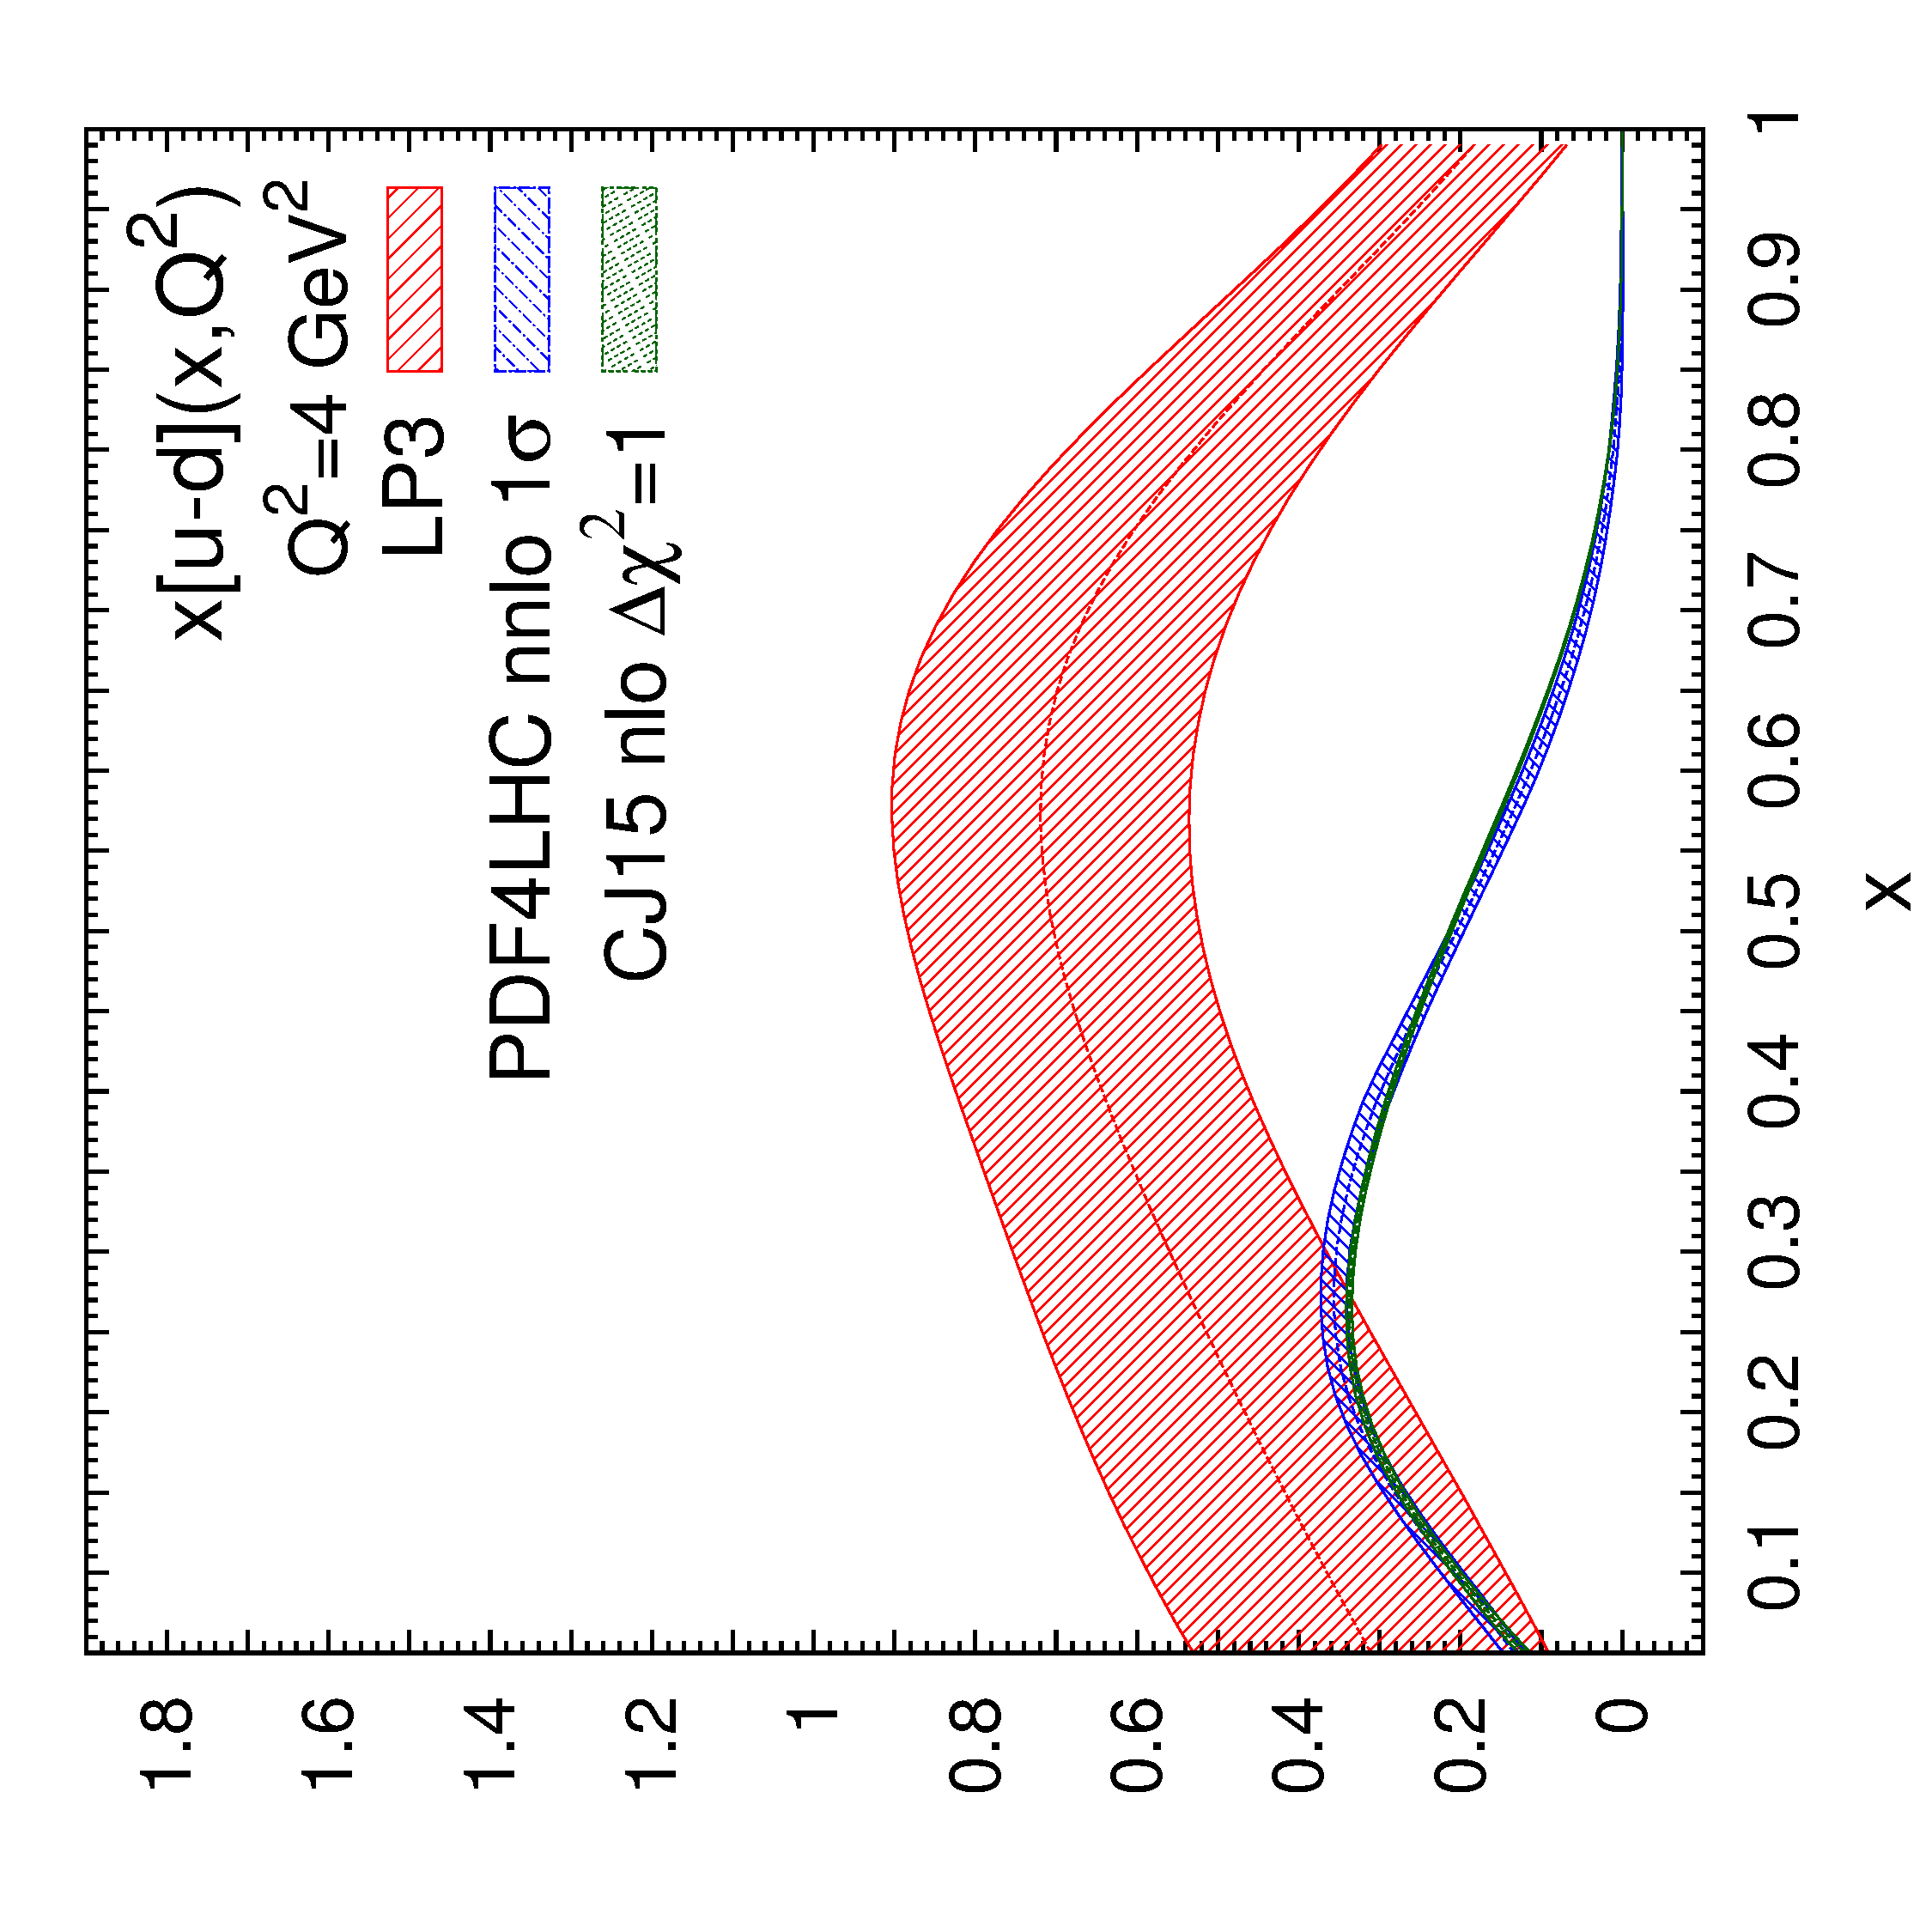
\includegraphics[scale=0.22,angle=270]{plots/unpxq}
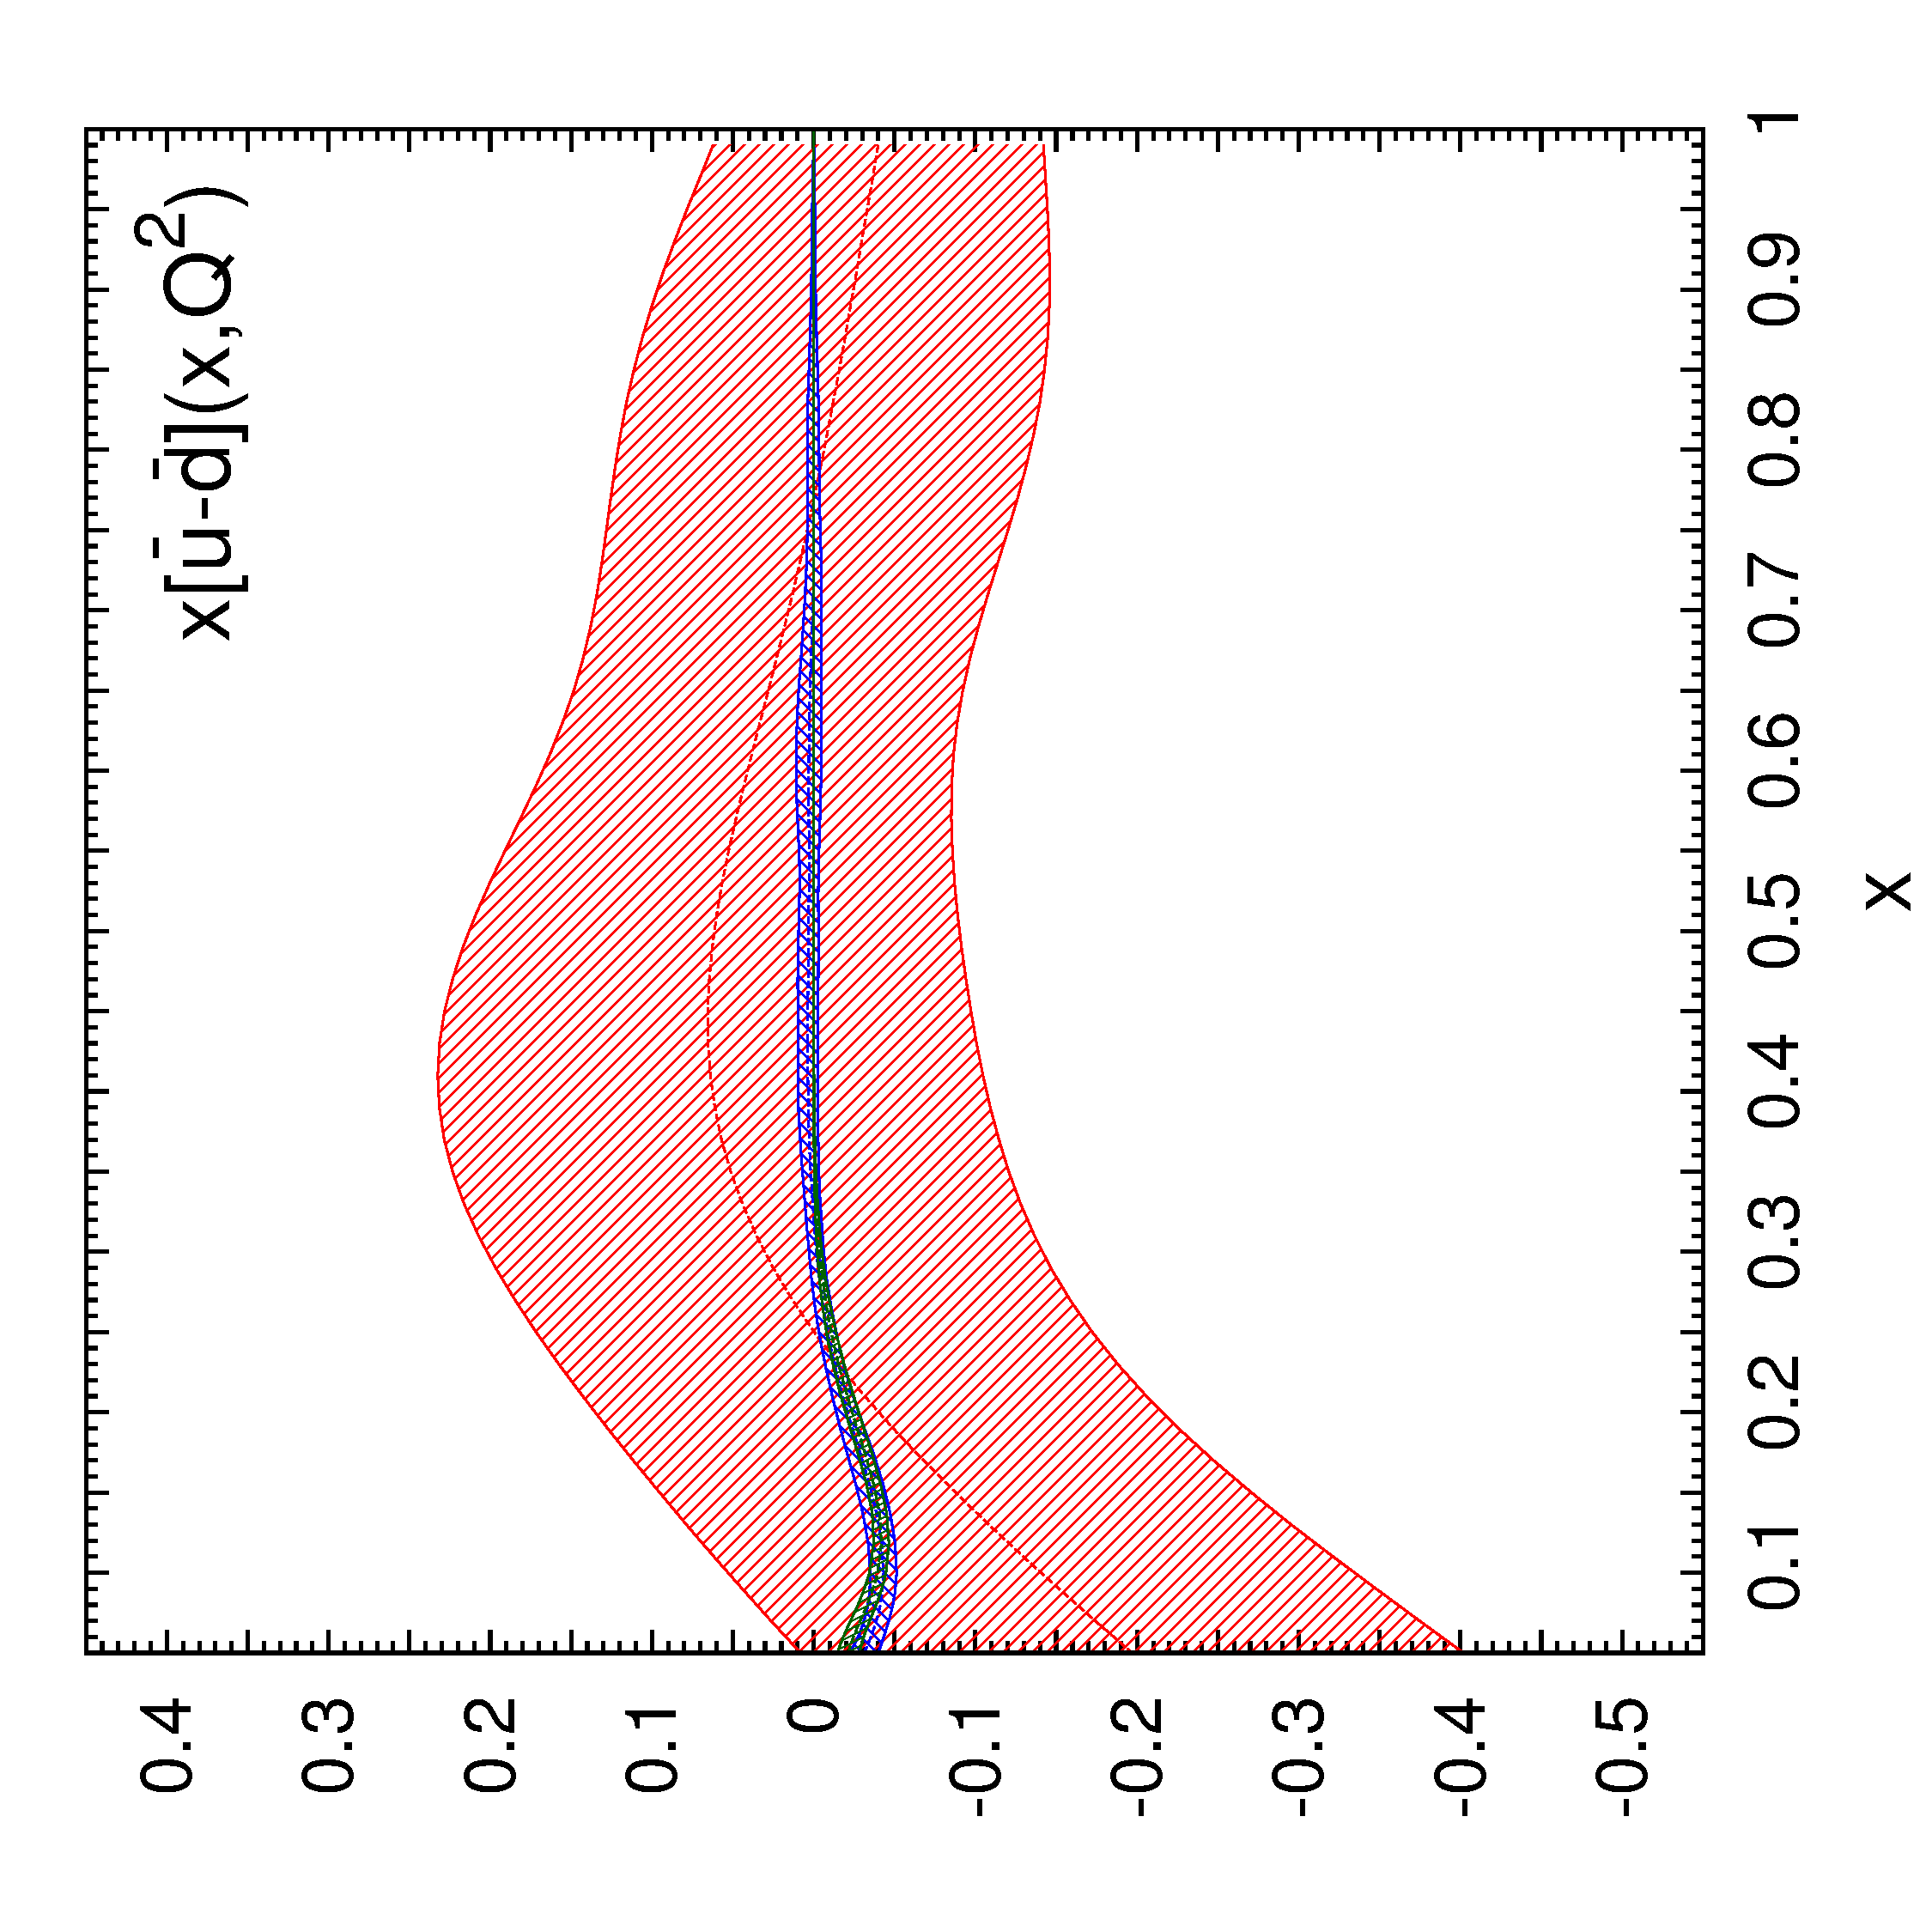
\includegraphics[scale=0.22,angle=270]{plots/unpxqbar}\\
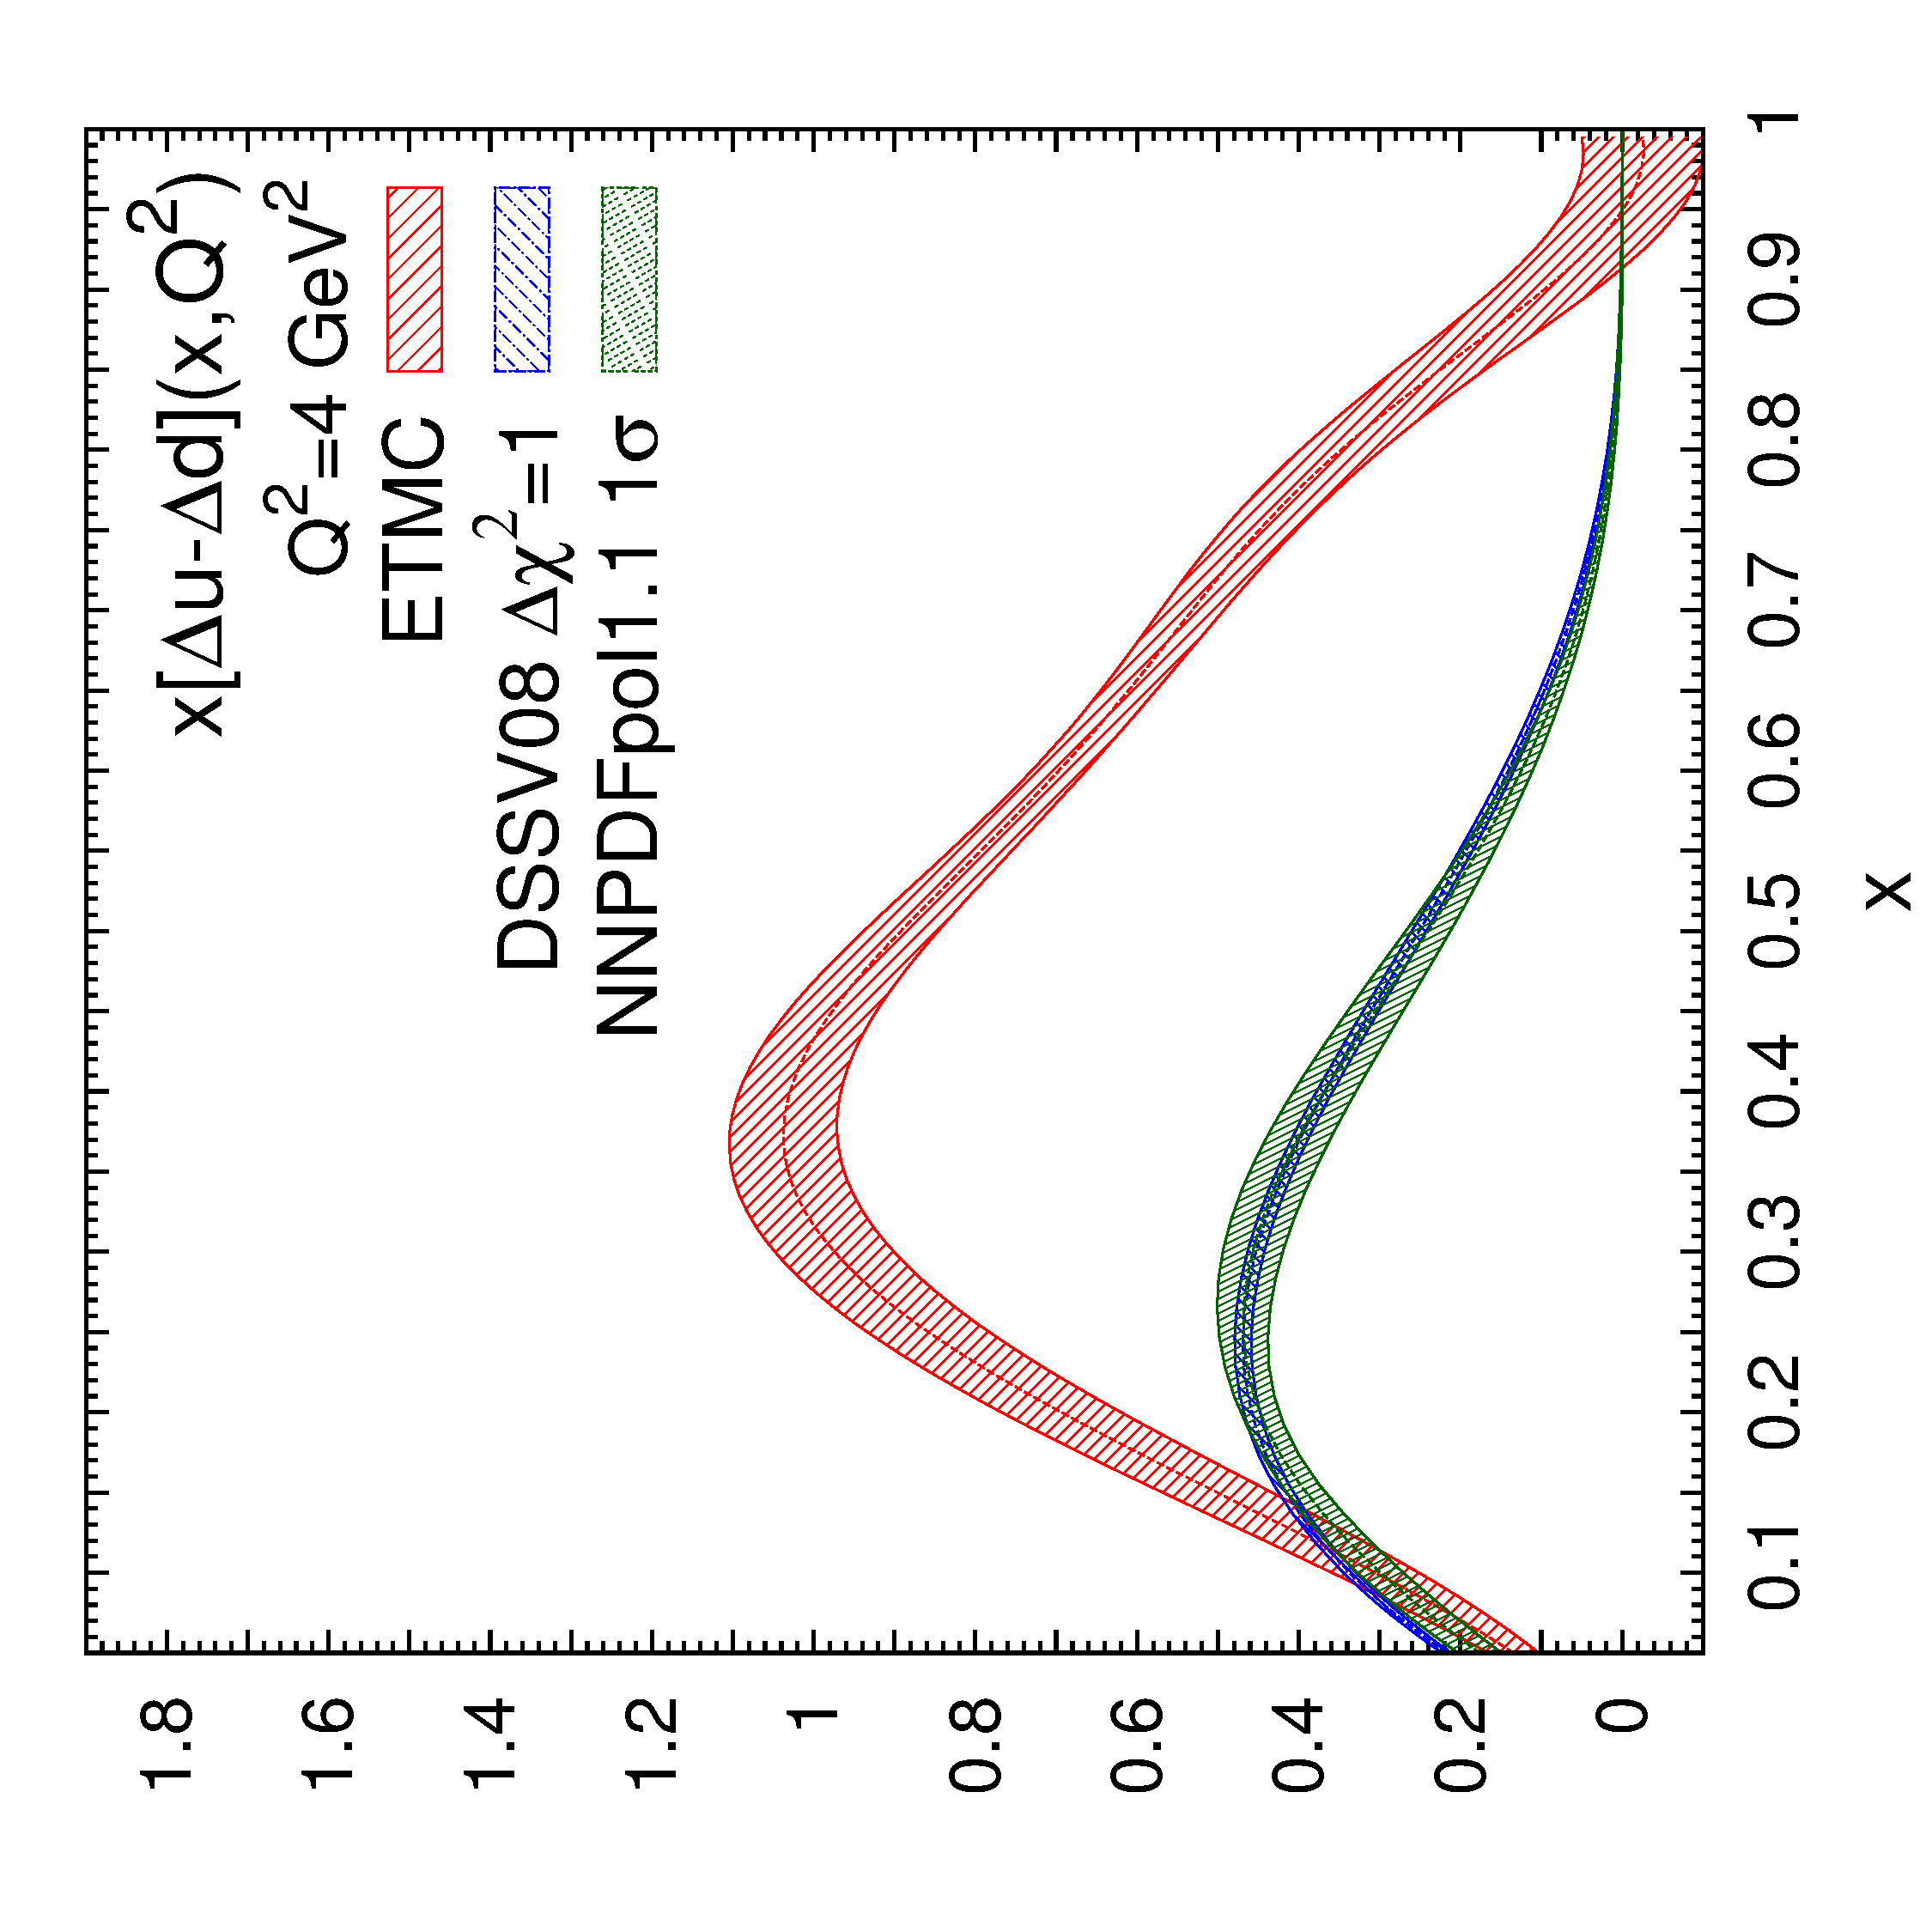
\includegraphics[scale=0.22,angle=270]{plots/polxq}
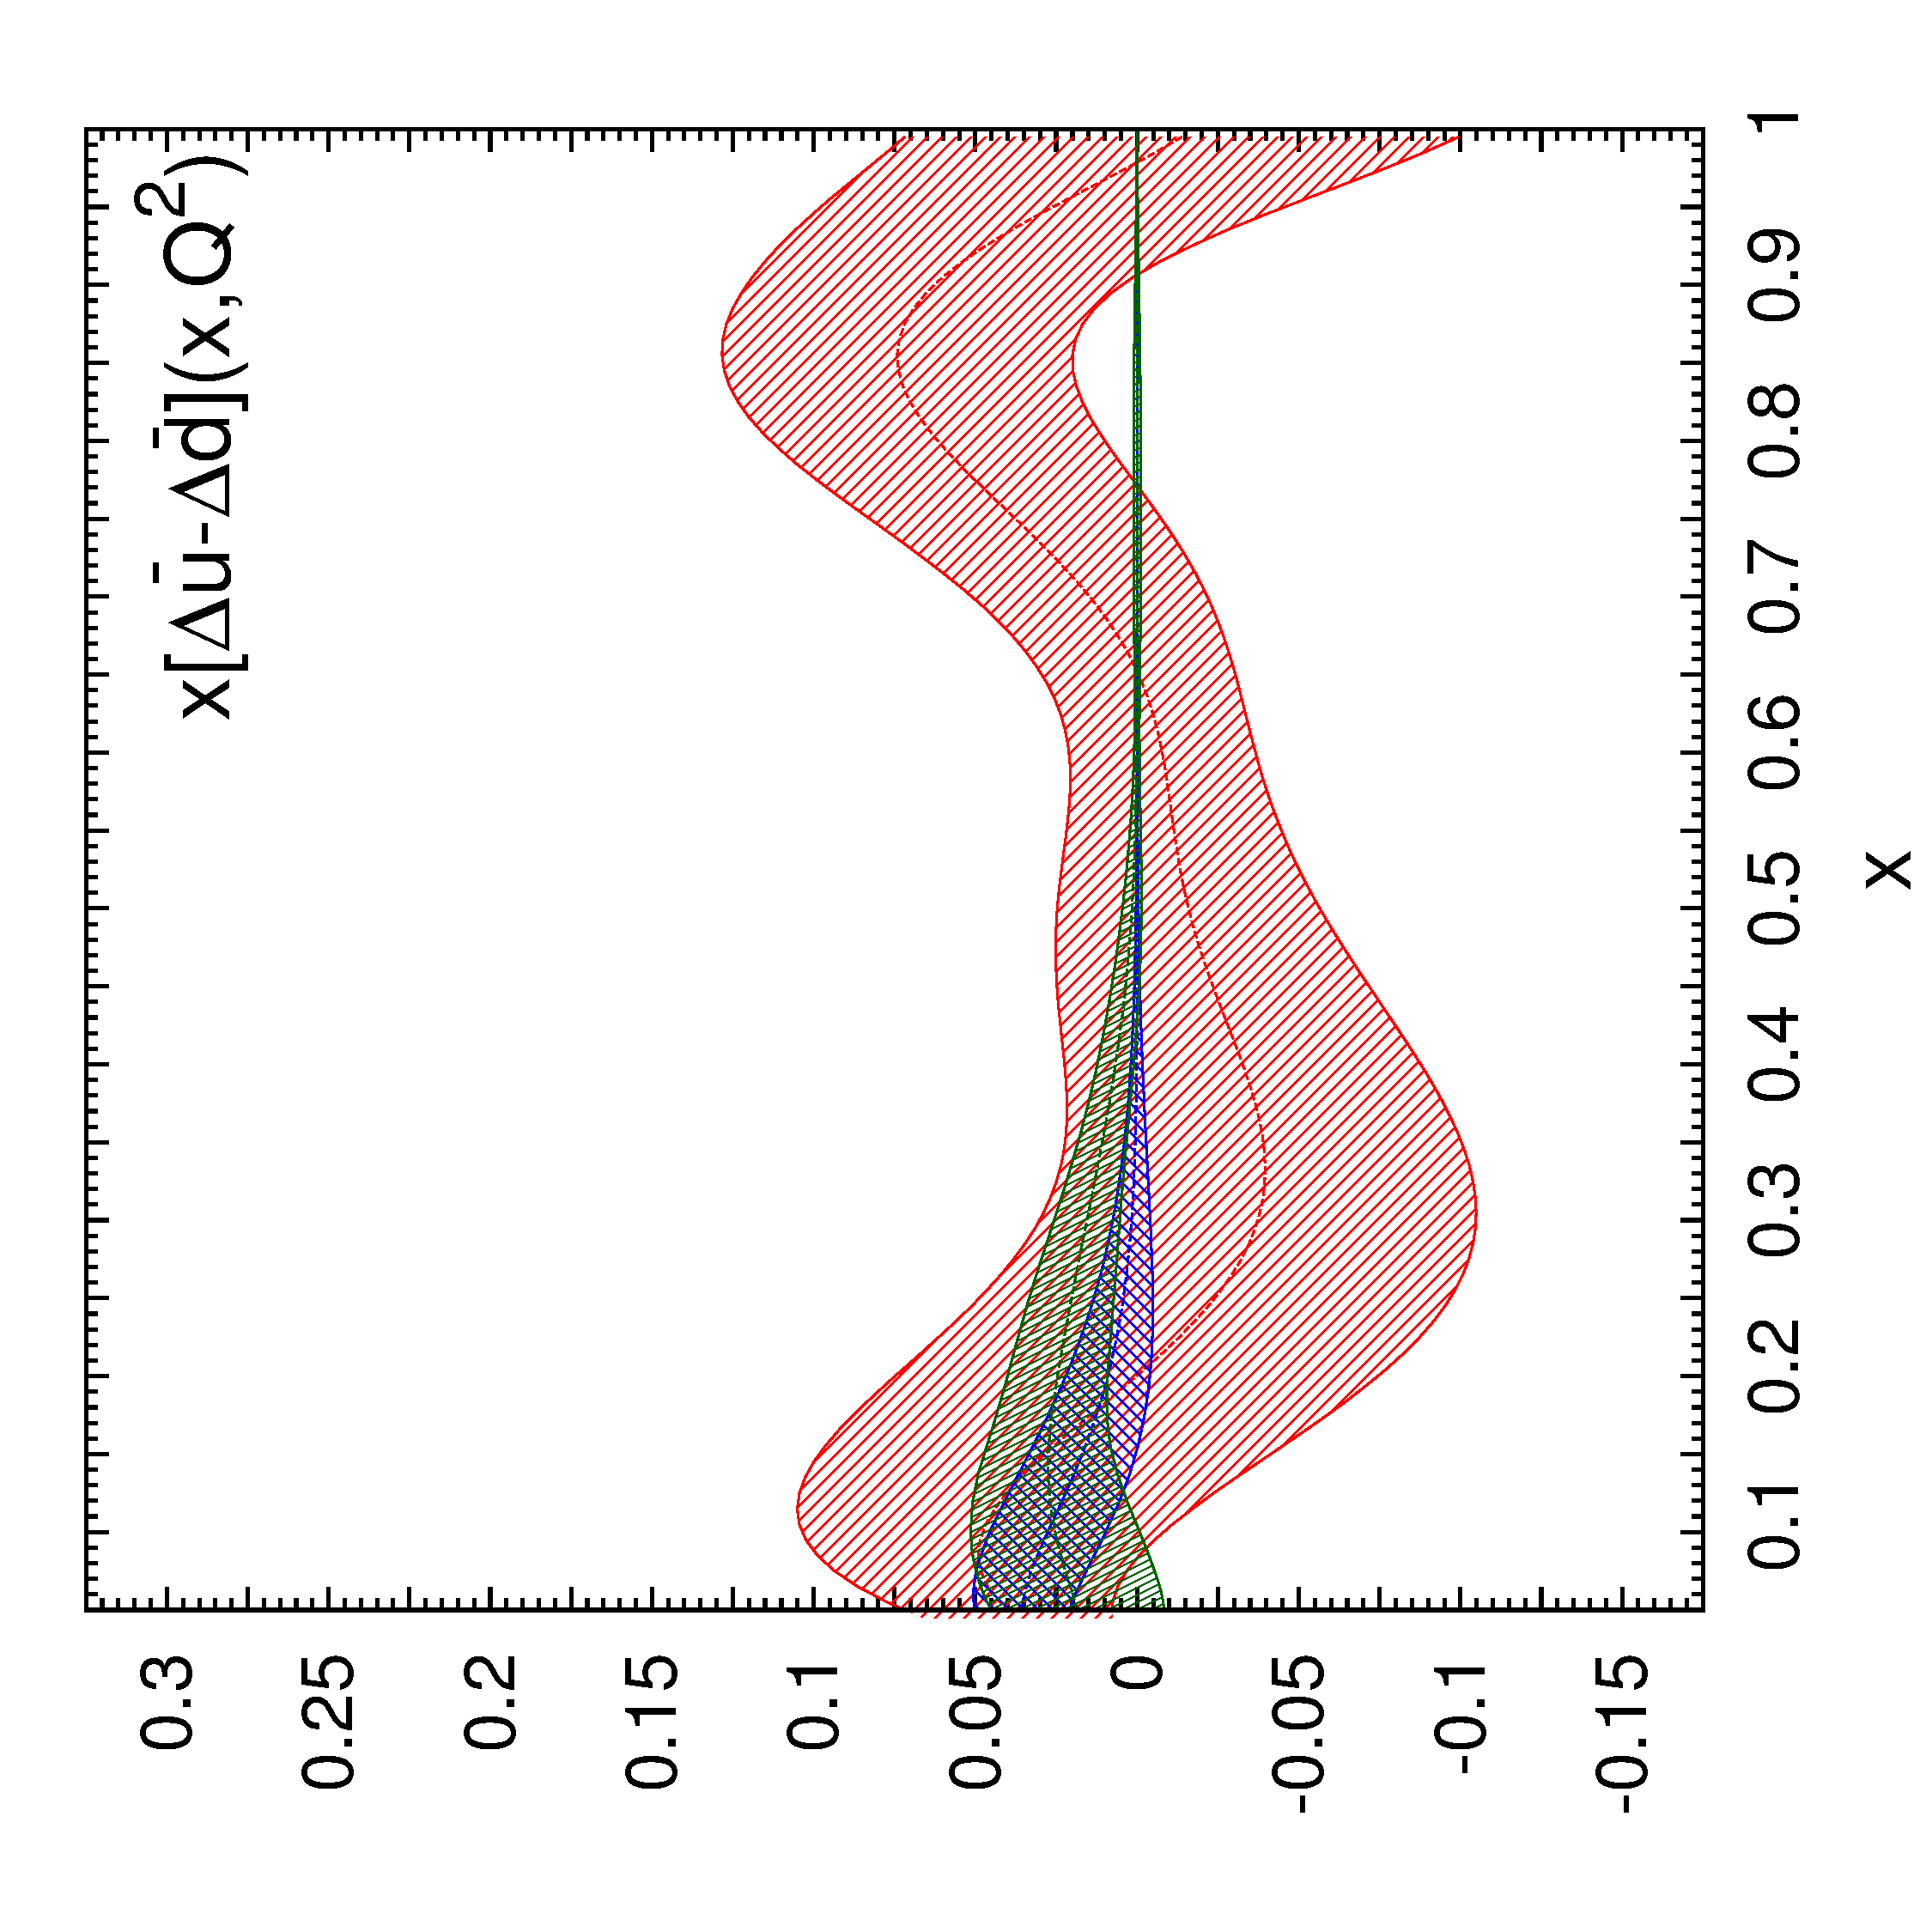
\includegraphics[scale=0.22,angle=270]{plots/polxqbar}\\
\caption{\small LP3's renormalized unpolarized isovector quark (top left) and 
  antiquark (top right) PDF combinations at physical pion mass with the renormalization scale 
  $\mu=2$~GeV~\cite{Lin:2017ani}. 
  %
  ETMC's renormalized polarized isovector quark (bottom left) and antiquark
  (bottom right) PDF combinations at pion mass of 
  375 MeV~\cite{Alexandrou:2017huk}.
  %
  Note that only statistical errors are shown here; the systematics are yet to be addressed. The small-x region (x< 0.2) can suffer larger systematics than the rest of the distribution due to the limited nucleon boost momentum.
  } 
\label{fig:qPDF-demo}
\end{figure}
%-------------------------------------------------------------------------------

\paragraph*{Pseudo-PDFs.} 
The general dependence of the  matrix element $h(z,p_z)$ of Eq.~\eqref{eq:qPDF} 
on the hadron momentum $p$ and the displacement of the quark and antiquark 
fields $z$ can be expressed as a function of the Lorentz invariants 
$\nu=z\cdot p$ (Ioffe time~\cite{Ioffe:1969kf,Braun:1994jq}) 
and $z^2$, where $z$ and $p$ are general 4-vectors.  
%
We can thus introduce
\begin{equation}
\overline{h}(\nu,z^2) \equiv h(z,p_z)\,.
\end{equation}

The pseudo-PDF is then defined by the Fourier transform
%
\begin{equation}
{\mathcal P}(x,z^2)=\int \frac{d\nu}{2\pi} e^{-ix\nu} \overline{h}(\nu,z^2),
\end{equation}
which has support only in the physical range 
$x=[-1,1]$ \cite{Radyushkin:2016hsy,Radyushkin:2017cyf}. 
%
As discussed in~\cite{Radyushkin:2016hsy,Radyushkin:2017cyf}, the pseudo-PDF 
is directly related to both the PDFs and the 
Transverse-Momentum-Dependent PDFs (TMDs).
%
In~\cite{Radyushkin:2017cyf}, using the temporal gamma matrix in the matrix 
element, a possible factorization of the TMD and PDF was conjectured which 
implies that the ratio
%
\begin{equation}
{\mathcal M}(\nu,z^2) =\frac{\overline h(\nu,z^2)}{\overline h(0,z^2)}
\label{eq:RatioPseudo}
\end{equation}
is directly related to the PDFs as 
\begin{equation}
{\mathcal M}(\nu,z^2) =Q(\nu,z^2) + {\cal O}(z^2).
\label{eq:IoffePDF}
\end{equation}
%
Here $Q(\nu,z^2)$ is the Ioffe time PDF~\cite{Ioffe:1969kf,Braun:1994jq}, 
which is just the Fourier transform of the PDFs,
\begin{equation}
{q}(x,1/z^2)=\int \frac{d\nu}{2\pi} e^{-ix\nu} Q(\nu,z^2).
\end{equation}
%
The ratio in Eq.~\eqref{eq:RatioPseudo} has a well-defined continuum 
limit and requires no renormalization. 
%
The polynomial corrections in Eq.~\eqref{eq:IoffePDF} are due to violations of 
the factorization conjecture, while the PDF ${q}(x,1/z^2)$ is the PDF in a 
particular scheme defined at scale $1/z^2$. Matching to $\overline{\rm MS}$ 
can be performed in perturbation theory following standard methodology. 
%
One loop results can be found in~\cite{Ji:2017rah,Radyushkin:2017lvu}.
%
A preliminary study was presented in~\cite{Orginos:2017kos,Karpie:2017bzm}, 
where it was shown that indeed the conjectured factorization is observed and 
the residual corrections are small. 
%
Further  evidence of the expected 
perturbative evolution of the Ioffe time PDFs was also observed. 
%
However, more detailed studies of this methodology are required.  


\subsection{Global PDF fits}
\label{Sec:IntroGlobalFits}

Now we move to present the state-of-the-art of global
unpolarized and polarized PDF fits, with emphasis on those
aspects of these analysis which have direct relevance for
the subsequent comparison with the lattice QCD calculations
that will be presented in the next section.

%%%%%%%%%%%%%%%%%%%%%%%%%%%%%%%%%%%%%%%%%%%%%%%%%%%%%%%
\subsubsection{Unpolarised PDFs}
\label{sec:unpPDFs}

Here we present the global PDF fitting framework,
starting with unpolarised PDFs, and then moving to polarized
PDFs.
%
We discuss in some technical detail how PDFs are extracted
from hard-scattering cross-sections, paying special attention
to the assessment of the PDF uncertainties.
%
We also briefly discuss the state of the art of unpolarised
global PDF fits.
%
Through this section,
we have made an effort to use a notation fully consistent
with the previous lattice QCD discussion.

\paragraph{General framework}
%
Unpolarised PDFs appear in the factorisation formulae for both
deep-inelastic scattering (DIS) and for proton-proton collisions.
%
The unpolarised DIS structure functions were defined in Eq.~\eqref{eq:Fi}.
%
For the hadroproduction of a generic final-state $X$ in $pp$ collisions, we have
a corresponding factorised expression
\begin{equation}
  \label{eq:LHCxsec}
\sigma_{pp\to X}(s,\mu_F,\mu_R)=\sum_{a,b}\int {\rm d}x_1 {\rm d}x_2\, f_a(x_1,\mu_F^2)f_b(x_2,\mu_F^2)\,\hat{\sigma}_{ab\to X}(x_1,x_2,s;\mu_{F},\mu_R)\;,
\end{equation}
where the hard cross section $\hat{\sigma}_{ab\to X}$ can
be calculated perturbatively as an expansion in the QCD and EW running couplings.
%
The specific values of the momentum fractions
$x_i$ are related to the kinematics of the final state.
%
In particular, at leading order it can be shown that
\be
x_{1,2}=\frac{M_X}{\sqrt{s}}e^{\pm y_X} \, ,
\ee
where $M_X$, $y_X$ are the invariant mass and rapidity of the produced system respectively.
%
The factorisation and renormalisation scales, $\mu_F$ and $\mu_R$, are taken to be of order the hard scale,
$\mu_F,\mu_R \sim Q$, of the process.

The DGLAP evolution equations of the PDFs, Eq.~(\ref{eq:dglap}), ensures that, when performing a global fit, the PDFs can be parameterised at one arbitrary input scale $Q_0\sim 1$ GeV, and
then be connected to any other higher scale $\mu$ that might be relevant
for comparisons with experimental data.
%
This input PDF parameterisation takes the generic form
\begin{equation}
\label{eq:pdffunc}
f_{i}(x,Q_0,\{a_i\})\sim x^{a_1}(1-x)^{a_2}\:C(x,\{a_j\})\, ,
\end{equation}
where the parameters $\{a_i\}$ determine the PDF shape
and are different for each PDF flavour combination that
is extracted from the data.
%
The $(1-x)^{a_2}$ term, with $a_{2}>0$, ensures that the PDFs
vanish in the elastic $x\to 1$ limit, as we would expect on basic physical grounds. 
%
Such a behaviour is also expected from the quark
counting rules~\cite{Brodsky:1973kr,Ball:2016spl}.
%
The $x^{a_1}$ term, which dominates in the low $x$
region, is expected from general Regge theory considerations,
although in modern fits the value of the power itself is left free.


The interpolating function $C(x)$ in
Eq.~(\ref{eq:pdffunc})
affects the behaviour of the PDFs away from the $x\to 0$ and 1
extrapolation regions.
%
This is assumed to be a smoothly varying function of $x$, for which a variety of choices have been made in PDF fits as we discuss below.
%
The heavy quark PDFs $c(x,\mu)$ and $b(x,\mu)$ are usually not
parametrised as in  Eq.~(\ref{eq:pdffunc}) but rather
generated by perturbative emission off gluons and light quarks,
though it is also possible to fit the charm PDF on an equal footing
to the light quarks~\cite{Ball:2016neh}.

While the general $x$ dependence of the PDFs is determined by
non-perturbative QCD dynamics, there are still a number
of theoretical constraints that any PDF set should satisfy and thus that
should be imposed during the global fit.
%
First of all, since
the proton has the quantum numbers of two up quarks and one down quark,
we have the following quark number sum rules given in terms of first
moments: 
%
\begin{eqnarray}
\int_{0}^{1}dx\ \left[u(x,\mu)-\bar{u}(x,\mu)\right] & =\left\langle 1\right\rangle _{u^{-}}= & 2 \, ,\nonumber \\
\int_{0}^{1}dx\ \left[d(x,\mu)-\bar{d}(x,\mu)\right] & =\left\langle 1\right\rangle _{d^{-}}= & 1 \, ,
\label{eq:valencesumrules}\\
\int_{0}^{1}dx\ \left[s(x,\mu)-\bar{s}(x,\mu)\right] & =\left\langle 1\right\rangle _{s^{-}}= & 0 \, ,\nonumber
\end{eqnarray}
with similar constraints for the heavy quarks: $\left\langle 1\right\rangle _{c^{-}}=\left\langle 1\right\rangle _{b^{-}}=\left\langle 1\right\rangle _{t^{-}}=0$.
%
Note that these constraints hold for any scale $\mu$, and indeed it can be shown
that if they hold at the input parametrisation scale $Q_0$, they
are subsequently respected by DGLAP evolution.
%
Therefore, for these valence distributions we must have $a_1>-1$ for the exponents in
Eq.~(\ref{eq:pdffunc}), else the valence sum rules would be ill-defined.

The second sum rule that we can impose on the PDFs arises
from the basic conservation of energy-momentum derived from
the QCD Lagrangian.
%
This so-called momentum sum rule arises
because the total
proton's momentum should be equal to the sum of the momentum
carried by all its constituents, namely
\begin{equation}\label{eq:mom}
1 = \left\langle x\right\rangle _{g}+\left\langle x\right\rangle _{u^{+}}+\left\langle x\right\rangle _{d^{+}}+\left\langle x\right\rangle _{s^{+}}+\left\langle x\right\rangle _{c^{+}}+\left\langle x\right\rangle _{b^{+}}+\left\langle x\right\rangle _{t^{+}}+\ldots\,,
\end{equation}
%
where the ellipsis represents any other partonic components (such
as a photon). The first moments, $\left\langle x\right\rangle _{f_i}$, are defined in analogy to Eq.~\eqref{eq:umoment1} and \eqref{eq:uplusmoment1}. Thus for non--valence distributions, we must have $a_1>-2$ to avoid a divergent contribution to
Eq.~\eqref{eq:mom}; typically we have $-2<_1a<-1$ for such distributions, and therefore for small $x$ the number of soft partons
grows very fast, although the momentum fraction carried by them is well-defined
and finite.
%
As in the case of the valence sum rules, the momentum
sum rule is also preserved by the DGLAP evolution equations.

As a representative illustration of the results of a global
PDF analysis, in Fig.~\ref{fig:nnlopdfs} we show
the results of the PDF4LHC15 NNLO set~\cite{Butterworth:2015oua}
both at a low scale
    $Q^2=10~{\rm GeV}^2$  and at a typical LHC scale
    $Q^2=10^4~{\rm GeV}^2$.
    %
    Specifically, we show the  $u_v=u-\bar{u}$ and $d_v=d-\bar{d}$ valence combinations, the $\bar{u}$,
    $\bar{d}$, $s$ and $c$ sea quark PDFs, and the gluon (divided by a factor 10).
    %
    Recall that the evolution between $Q^2=10$ to $Q^2=10^4~{\rm GeV}^2$ is completely
    determined by the solution of
     the DGLAP evolution equations.
    %
    Note how the shape of the $u_v~(u^{-})$ and $d_v~(d^{-})$ valence quark combinations
    reflects the constraints from the valence sum rules Eq.~(\ref{eq:valencesumrules}).
    %
    At small $x$, there is a rapid growth of the gluon and the sea quark PDFs, implying
    that the higher the collision center-of-mass energy $\sqrt{s}$, the more
    important gluon- and sea-quark-initiated processes become.
    %
    The bands in Fig.~\ref{fig:nnlopdfs} represent the 68\% confidence level
    PDF uncertainties, determined as discussed below.

%%%%%%%%%%%%%%%%%%%%%%%%%%%%%%%%%%%%%%%%%%%%%%%%%%%%%%%%%%%%%%%%%%%%%
\begin{figure}[t]
\begin{center}
  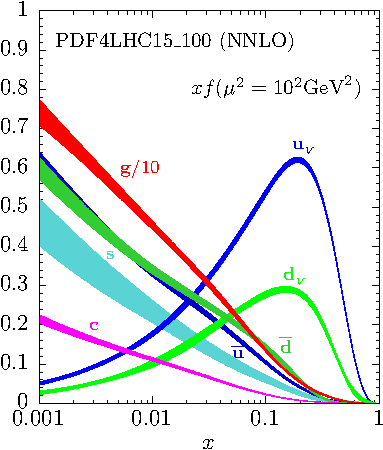
\includegraphics[scale=1.2]{plots/pdf4lhcq10.pdf}
  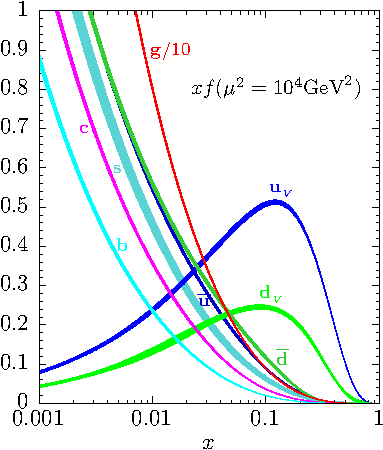
\includegraphics[scale=1.2]{plots/pdf4lhcq1000.pdf}
  \caption{\small The PDF4LHC15 NNLO PDFs at a low scale
    $Q^2=10~{\rm GeV}^2$ (left plot) and at a typical LHC scale
    $Q^2=10^4~{\rm GeV}^2$ (right plot) as a function of $x$.
    %
    We show the $u_v$ and $d_v$ valence combinations, the $\bar{u}$,
    $\bar{d}$, $s$ and $c$ sea quark PDFs, and the gluon (note that
    the latter is divided by a factor 10).
    \label{fig:nnlopdfs}
  }
\end{center}
\end{figure}
%%%%%%%%%%%%%%%%%%%%%%%%%%%%%%%%%%%%%%%%%%%%%%%%%%%%%%%%%%%%%%%%%%%%%%

Following this initial introduction, we move to describe in some more detail
the most important ingredients of a global PDF analysis.

\paragraph*{Fitting PDFs from hard-scattering data}
%
The global PDF analysis framework is based on a combination of three basic components: experimental
data, perturbative calculations, and fitting methodology, which we now describe
in turn.

\begin{enumerate}
\item A broad set of input hard-scattering cross-sections from DIS and proton-proton collisions, providing information on the PDFs
  over a wide range of $x$ and for different flavour combinations.
  %
  While traditional PDF fits were based mostly on DIS structure function and Drell-Yan
  and inclusive jet
  cross-sections, in the recent years many other processes have demonstrated
  their usefulness for constraining PDFs, from top-quark pair production~\cite{Czakon:2016olj}
  to the $p_T$ of $Z$ bosons~\cite{Boughezal:2017nla}
  and $D$ meson production in the forward region~\cite{Gauld:2016kpd}, among
  several others.

  In Fig.~\ref{fig:kinplot-report} we show the representative kinematic coverage in the
    $(x,Q^2)$ of the DIS and proton-proton hard-scattering measurements that are
    used as input in a global unpolarised PDF fit, in this case NNPDF3.1~\cite{Ball:2017nwa}.
    %
    In order to facilitate visualisation, different
    datasets have been clustered together into families of
    related processes.
    %
      For hadronic cross-sections, leading order kinematics are assumed to map
    each experimental bin to a pair of points in the $(x,Q^2)$ plane.
    %
    We observe that the current dataset extends down to $x\simeq 5\cdot 10^{-5}$
    at low $x$, and up to few TeV at high $Q$.
    %
    The fact that similar regions in the $(x,Q)$ plane are covered by
    different processes is essential in order to achieve quark
    flavour separation and to constrain the gluon PDF.

%%%%%%%%%%%%%%%%%%%%%%%%%%%%%%%%%%%%%%%%%%%%%%%%%%%%%%%%%%%%%%%%%%%%
\begin{figure}[t]
\begin{center}
  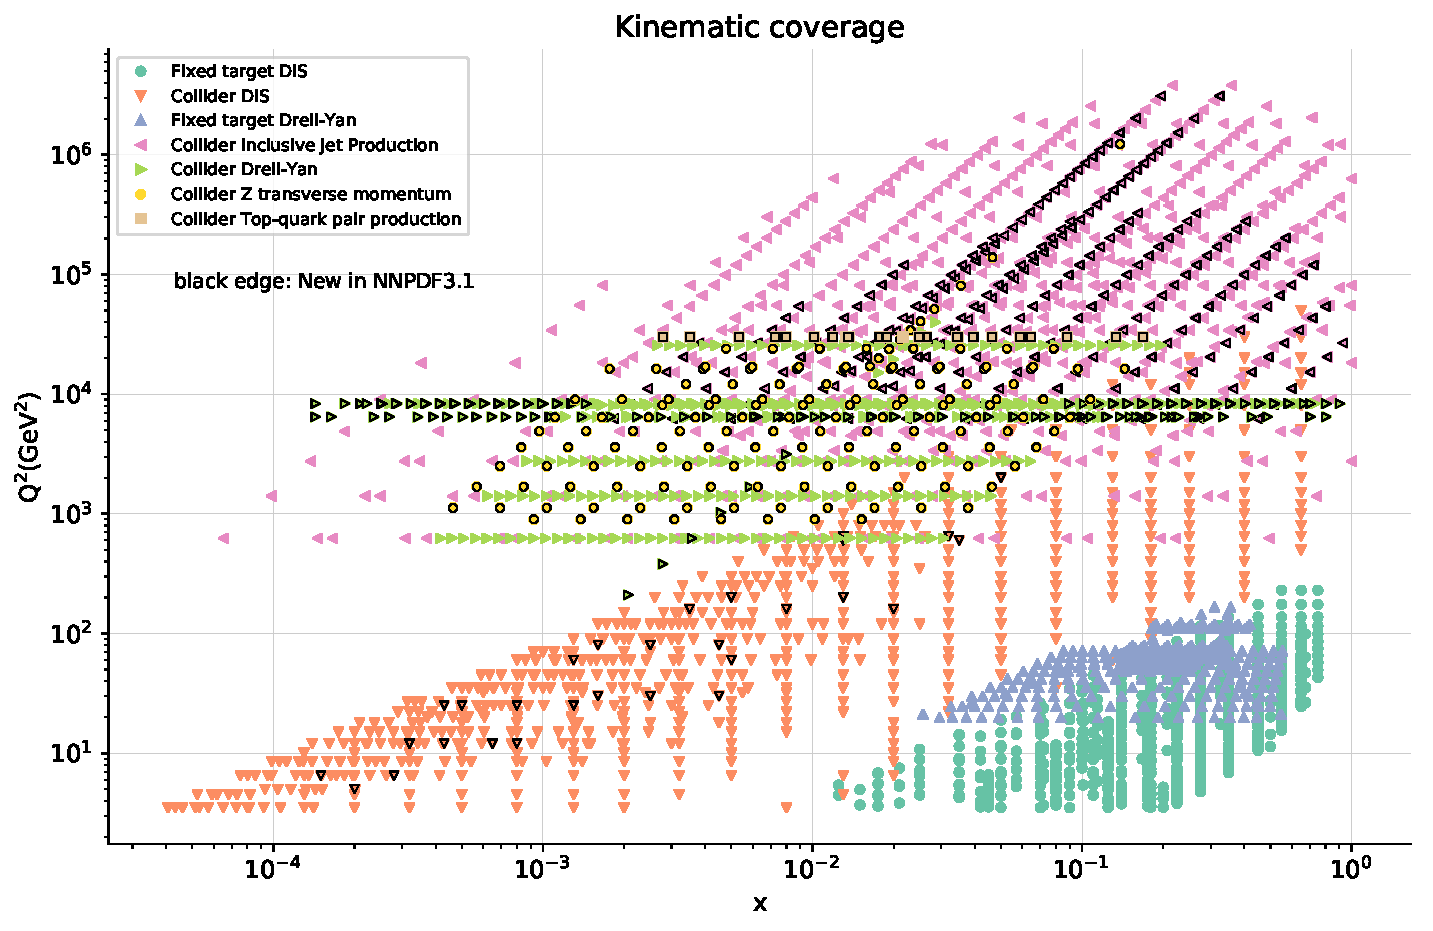
\includegraphics[scale=0.60]{plots/kinplot-report.pdf}
  \caption{\small Representative kinematical coverage in the
    $(x,Q^2)$ of the DIS and proton-proton hard-scattering measurements that are
    used as input in a global unpolarised PDF fit, in this case NNPDF3.1~\cite{Ball:2017nwa}.
    %
    In order to facilitate visualisation, different
    datasets have been clustered together into families of
    related processes.
    %
    For hadronic cross-sections, leading order kinematics are assumed to map
    each experimental bin to a pair of points in the $(x,Q^2)$ plane.
    \label{fig:kinplot-report} 
  }
\end{center}
\end{figure}
%%%%%%%%%%%%%%%%%%%%%%%%%%%%%%%%%%%%%%%%%%%%%%%%%%%%%%%%%%%%%%%%%%%%%

  \item Theoretical calculations of DIS and hadronic cross-sections
    for the highest perturbative order available.
    %
    Currently, this implies using NNLO for the QCD corrections and NLO
    for the electroweak and photon-induced effects~\cite{Manohar:2016nzj,Manohar:2017eqh}.
    %
    Thanks to recent progress in higher-order calculations, these results
    are available for most of the processes entering the global
    PDF fits~\cite{Currie:2016bfm,Campbell:2016lzl,Czakon:2016dgf,Boughezal:2017nla,Li:2012wna},
    including differential distributions with coloured particles
    in the final state.

    Crucially, these calculations should be provided in
    a format such that the evaluation of the hadronic
    cross-sections Eq.~(\ref{eq:LHCxsec}) is not too burdensome
    from a computational point of view.
    %
    To bypass the limitations of the lengthy (N)NLO
    computations, a number of fast interfaces have
    been developed that allow the efficient calculation
    of NLO (and NNLO) fully differential hadronic cross-sections.
    %
    The exploitation of fast interfaces such as {\tt APPLgrid}~\cite{Carli:2010rw},
    {\tt FastNLO}~\cite{Wobisch:2011ij} and {\tt aMCfast}~\cite{Bertone:2014zva} is of utmost importance
    for modern PDF fits, given the wealth of collider data used.

  \item A fitting methodology that determines the best-fit
    PDF parameters and their uncertainty from the minimisation
    of a suitable statistical estimator, typically the $\chi^2$
    or a related estimator.
    %
    There exist different alternative definitions of the $\chi^2$
    to be used in the global fit~\cite{Ball:2012wy}, for instance one frequently
    used definition is
    \begin{equation}
\chi^2 = \sum_{i,j}^{N_{\rm dat}} (T_i(\{a_k\}) - D_i) ({\rm cov^{-1}})_{ij} (T_j(\{a_k\}) - D_j),
\label{eq:chi2}
    \end{equation}
    where $N_{\rm dat}$ is the number of data points of a given experiment,
    and $T_i$ and $D_i$ are the corresponding theoretical calculations
    and the central values of the experimental data, respectively.
    %
    The theoretical predictions $T_i(\{a_k\})$ depend on the input
    PDF parametrisation, and thus on the fitting parameters,
    see Eq.~\eqref{eq:pdffunc}.
    %
    Therefore, Eq.~\eqref{eq:chi2} can be used as a figure of merit to
    assess the agreement between theory
    and data.

    The covariance matrix $({\rm cov})_{ij}$
    accounts for the various sources of experimental
    systematic uncertainties and
    also accepts several
    different definitions.
    %
    One example is the so-called
 $t_{0}$-prescription~\cite{Ball:2009qv}, 
where a fixed theory prediction $T_{i}^{(0)}$
is used to define the  contribution to the $\chi^2$
from the multiplicative systematic uncertainties, namely
\be
\label{eq:covmat_t00}
({\rm cov})_{ij}=
\delta_{ij} \sigma_{\rm stat}^2 + 
\sum_{\alpha=1}^{N_c}\sigma^{(c)}_{i,\alpha}\sigma^{(c)}_{j,\alpha}D_{i} D_{j}
+ \sum_{\beta=1}^{N_{\cal L}} \sigma_{i,\beta}^{({\cal L})}\sigma_{j,\beta}^{({\cal L})}
T^{(0)}_{i} T^{(0)}_{j}\, .
\ee
Here $\sigma_{\rm stat}$ is the uncorrelated uncertainty,
and $\sigma^{(c)}_{i,\alpha}$ ($\sigma^{(\cal L)}_{i,\beta}$)
are the various sources of additive (multiplicative) systematic uncertainties.

Note that so far theoretical uncertainties, such as those arising
from missing higher orders (MHO) in the perturbative
expansion, are not included in the $\chi^2$ definition
used in current PDF fits.

\end{enumerate}

The goal of a global PDF fit is therefore to combine together
all available hard-scattering data with the
corresponding higher-order theoretical
calculations in order to determine
the best-fit shape of the PDFs by means of the minimisation
of the $\chi^2$ estimator Eq.~(\ref{eq:chi2}).
%
Moreover, it is not enough to determine the best-fit values of
the PDF parameters: we also need to estimate the associated PDF
uncertainties, as we discuss next.


\paragraph{PDF uncertainties}
%
A central ingredient of the global PDF fitting framework is the determination
of the various sources of experimental, theoretical and
methodological uncertainties that affect the best-fit PDFs.
%
In this respect,
there are two main methods to determine PDF uncertainties, the {\it
  Hessian} and the {\it Monte Carlo} methods,\footnote{The Lagrange Multiplier
  method~\cite{Stump:2001gu} is also frequently used for dedicated studies of
  PDF uncertainties for specific cross-sections.} which we briefly
review now:
\begin{itemize}
\item The Hessian method~\cite{Pumplin:2001ct} is based on the parabolic
expansion of the $\chi^2$ in the vicinity of the minimum, parametrised
by a number of orthogonal eigenvectors within some fixed tolerance.
%
The basic idea of this method is that
in the vicinity of this minimum, the $\chi^2$ can
be approximated in terms of a quadratic expansion,
\be
\label{eq:hessianexpansion}
\Delta\chi^2 \equiv \chi^2- \chi^2_{\rm min}
=\sum_{i,j=1}^{n_{\rm par}}H_{ij}\lp a_i-a_i^0\rp
\lp a_j-a_j^0\rp \, ,
\ee
where the $n_{\rm par}$ PDF fit parameters are denoted by $\{a_1,\ldots,
a_{n_{\rm par}}\}$, the best-fit values that minimise the
$\chi^2$ are indicated by
$\{a_1^0,\ldots,
a^0_{n_{\rm par}}\}$,
and the Hessian matrix is defined as
\be
H_{ij}\equiv \frac{1}{2} \frac{\partial^2\chi^2}{\partial a_i
\partial a_j}\Bigg|_{\{\vec{a}\}=
\{\vec{a^0}\}} \, .
\ee
By diagonalising this Hessian matrix,
it becomes possible
to represent
PDF uncertainties in terms of orthogonal eigenvectors.
%
These eigenvectors
can then be used to estimate the PDF uncertainty
for arbitrary cross-sections, using the master formula
of Hessian PDF sets for the uncertainty of the cross-section
$\mathcal{F}$, namely
\be
\label{eq:hessianmaster2}
\sigma_{\mathcal{F}}=\frac{1}{2}\lp \sum_{i,j}^{n_{\rm par}}
\lc \mathcal{F}(S_i^+)-\mathcal{F}(S_i^-) \rc \rp^{1/2} \, ,
\ee
where $S_i^{\pm}$ correspond to the $i$-th eigenvector
associated to positive and negative variations with respect
to the best fit value.

\item The Monte Carlo method~\cite{Forte:2002fg,DelDebbio:2004xtd} is based 
  on constructing a representation
  of the probability distribution of the experimental data in terms
  of a large number  $N_{\rm rep}$ of {replicas}, and
 PDF fits are then performed separately on each of these Monte Carlo replicas.
%
With this construction, the resulting ensemble of PDFs represents the probability density in the space
of parton distributions.
%
This requires generating a large number of artificial replicas $N_{\rm rep}$
of the original data which encode the same information on
central values, variances and correlations as that provided by the experiments.

Specifically, given an experimental measurement of a hard-scattering
cross-section denoted generically by $F_{I}^{\rm (exp)}$ with
total uncorrelated uncertainty $\sigma_{I}^{\rm (stat)}$, $N_{\rm sys}$ fully
correlated systematic uncertainties $\sigma^{\rm (corr)}_{I,c}$ and
$N_a$ ($N_r$) absolute (relative) normalisation uncertainties
$\sigma^{\rm (norm)}_{I,n}$, the artificial
MC replicas are constructed using the following expression
\be
\label{eq:replicas}
F_{I}^{(\art)(k)}=S_{I,N}^{(k)} F_{I}^{\rm (\mrexp)}\lp 1+
 \sum_{c=1}^{N_{\rm sys}}r_{I,c}^{(k)}\sigma^{\rm (corr)}_{I,c}+r_{I}^{(k)}\sigma_{I}^{\rm (stat)}\rp
 \ , \quad k=1,\ldots,N_{\rep} \ ,
\ee
where $S_{I,N}^{(k)}$ is the normalisation prefactor.
%
Here the variables $r_{I,c}^{(k)},r_{I}^{(k)},r_{p,n}^{(k)}$ are
 univariate Gaussian random numbers.
 %
 For each individual replica, the random fluctuations
 associated to a given fully-correlated systematic
 uncertainty will be the same
 for all data points, $r^{(k)}_{I,c}=r^{(k)}_{I',c}$.

 Within the Monte Carlo method, the expectation function of a generic
cross-section $ \mathcal{F} [ \{  q \}]$
is evaluated as an average over the replica sample,
\be
\label{masterave}
\la \mathcal{F} [ \{  q \}] \ra
= \frac{1}{N_{\rm rep}} \sum_{k=1}^{N_{\rm rep}}
\mathcal{F} [ \{  q^{(k)} \}] \, ,
\ee
and the corresponding one-sigma
uncertainty is then determined as the variance of the
Monte Carlo sample,
\be
\sigma_{\mathcal{F}} =
\left( \frac{1}{N_{\rm rep}-1}
\sum_{k=1}^{N_{\rm rep}}   
\lp \mathcal{F} [ \{  q^{(k)} \}] 
-   \la \mathcal{F} [ \{  q \}] \ra\rp^2 
 \right)^{1/2}.
\label{mastersig}
\ee
It is also straightforward to compute other properties of the
underlying PDF probability distribution such as higher moments
like skewness and kurtosis.

\end{itemize}

In the following sections
of this document, when comparing the results of global PDF fits
with the results of lattice QCD calculations we will use Eqs.~(\ref{eq:hessianmaster2}) and~(\ref{mastersig})
to evaluate the PDF uncertainties of Hessian and Monte Carlo PDF sets, respectively.
%
Unless otherwise state, the quoted PDF uncertainties correspond to the 68\% confidence
level intervals.
%
Note that given a PDF set in the Hessian representation, it is possible to construct
the corresponding Monte Carlo representation~\cite{Watt:2012tq,Hou:2016sho}
and vice-versa~\cite{Gao:2013bia,Carrazza:2015aoa}.

It is important to emphasise here that there are additional sources of theoretical
uncertainty that are not accounted for, either in the Hessian or
in the MC methods.
%
The first one is the parametric uncertainty due to finite uncertainties associated
with the input values of the physical parameters used in the global fit, such
as $\alpha_s(m_Z)$ and the charm mass $m_c(m_c)$.
%
These additional uncertainties can be included by repeating the fits for different values of the
physical parameters and then suitably combining the results.
%
The second source of theoretical uncertainty neglected in PDF fits
is that due to the truncation of the perturbative expansion, known
as missing higher-order uncertainty (MHOU).
%
While this is expected to be small for NNLO fits, currently its size is unknown.
This should be taken into account when comparing global extractions of PDFs with lattice
QCD results, which represent, in some sense, an ``all-order'' computation.

\paragraph{State-of-the-art global PDF fits}
%
Various collaborations provide regular updates of their global unpolarised
PDF fits.
%
The latest fits from the three main global fitting collaborations
are CT14~\cite{Dulat:2015mca}, MMHT14~\cite{Harland-Lang:2014zoa} and
NNPDF3.1~\cite{Ball:2017nwa}.
%
These fits are performed up to NNLO in the strong coupling (with central value
$\alpha_s(m_Z)=0.118$),
and include data from the HERA $e^{\pm} p$ collider, fixed (nuclear and proton) target experiments, the Tevatron $p\overline{p}$ collider and the LHC. 
%
The ABMP16~\cite{Alekhin:2017kpj} set fits to a similar global data set
(although excluding jet production)
but differs in its treatment of errors and heavy flavours.
%
The HERAPDF2.0~\cite{Abramowicz:2015mha} set fits to the final combined HERA Run I + II data set only, with the aim of determining the PDFs from a completely consistent DIS data sample; in $x$ regions that are less constrained by HERA data, the uncertainties can be quite large.
%
The CJ15~\cite{Accardi:2016qay} NLO set focuses on constraining the PDFs at higher $x$ by lowering $Q^2$ and $W^2$ cuts in DIS.
%
This greatly increases the available data, but requires additional modeling of power--like ${\cal O}(1/Q^2)$ corrections.

A detailed discussion of the similarities and differences between
PDF sets, which is beyond the scope of this document,
can be found in the PDF4LHC report~\cite{Butterworth:2015oua}.
%
It suffices here to say that all PDF sets listed above use the Hessian
method to determine PDF uncertainties,
except NNPDF which instead
is based on the Monte Carlo approach.

As discussed above, in order to perform a  PDF fit, some form for the interpolating function $C(x)$ in Eq.~\eqref{eq:pdffunc}
must be assumed.
%
The simplest ansatz, which has been very widely used, is to take a basic polynomial form in $x$ (or $\sqrt{x}$), such as
\begin{equation}\label{eq:lpower}
C(x)=1+a_2\sqrt{x}+a_3 x+...\;.
\end{equation}
Functional forms of this type are for example taken by CJ, HERAPDF and earlier MMHT and CT sets. More recently, the CT and MMHT collaborations instead expand in terms of a basis of  Bernstein and Chebyshev polynomials, respectively.
%
While formally equivalent to the simple polynomial expansion
Eq.~\eqref{eq:lpower}, these are much more convenient for fitting as the number of free parameters $n_{\rm par}$ is increased.
%
In the latest CT and MMHT sets, there are between 20 and 40 free parameters in total,
though some of these are kept fixed when evaluating the
Hessian PDF uncertainties.

An alternative approach to the PDF parametrisation is adopted
by the NNPDF collaboration. Here, the interpolating function is modelled with a multi--layer feed forward neural network.
%
In practice, this allows for a greatly increased number of free parameters, typically an order of magnitude higher than other sets.
%
The form of Eq.~\eqref{eq:pdffunc} is still assumed, but
now $C(x)={\rm ANN}(x)$ is parametrised as an artificial
neural network.
%
The $x^{a_1}(1-x)^{a_2}$ term that multiplies the ANN represents
a pre--processing factor that speeds up the minimisation procedure
and that is determined via an iterative procedure.

In Fig.~\ref{fig:globalfits}
we present a snapshot of our current understanding
of the proton structure in the global PDF fitting framework.
%
We compare the CT14, MMHT2014
  and NNPDF3.1 NNLO PDF sets at $Q=100$ GeV, normalised
  to the central value of the latter.
  %
  From top to bottom and from left to right we show the
  $u$, $\bar{d}$ and $s$ quark PDFs as well as the gluon.
  %
  The error bands indicate the 1-$\sigma$ PDF uncertainties
  associated to each set, computed with the corresponding
  master formula.
  %
  We observe that differences for the up quark PDF
  are small, at the few percent level, but greater differences
  are observed for the sea quarks, in particular
  in the medium and large-$x$ region.
  %
  For the gluon there is reasonable agreement except
  in the large-$x$ region, where NNPDF3.1 is softer than
  CT14 and MMHT14.
%
We note that any other comparison plot between PDFs can be straightforwardly
obtained using the {\tt APFEL-Web} online plotting interface~\cite{Carrazza:2014gfa}.

%%%%%%%%%%%%%%%%%%%%%%%%%%%%%%%%%%%%%%%%%%%%%%%%%%%%%%%%%%%%%%%%%%%%%
\begin{figure}[t]
  \begin{center}
 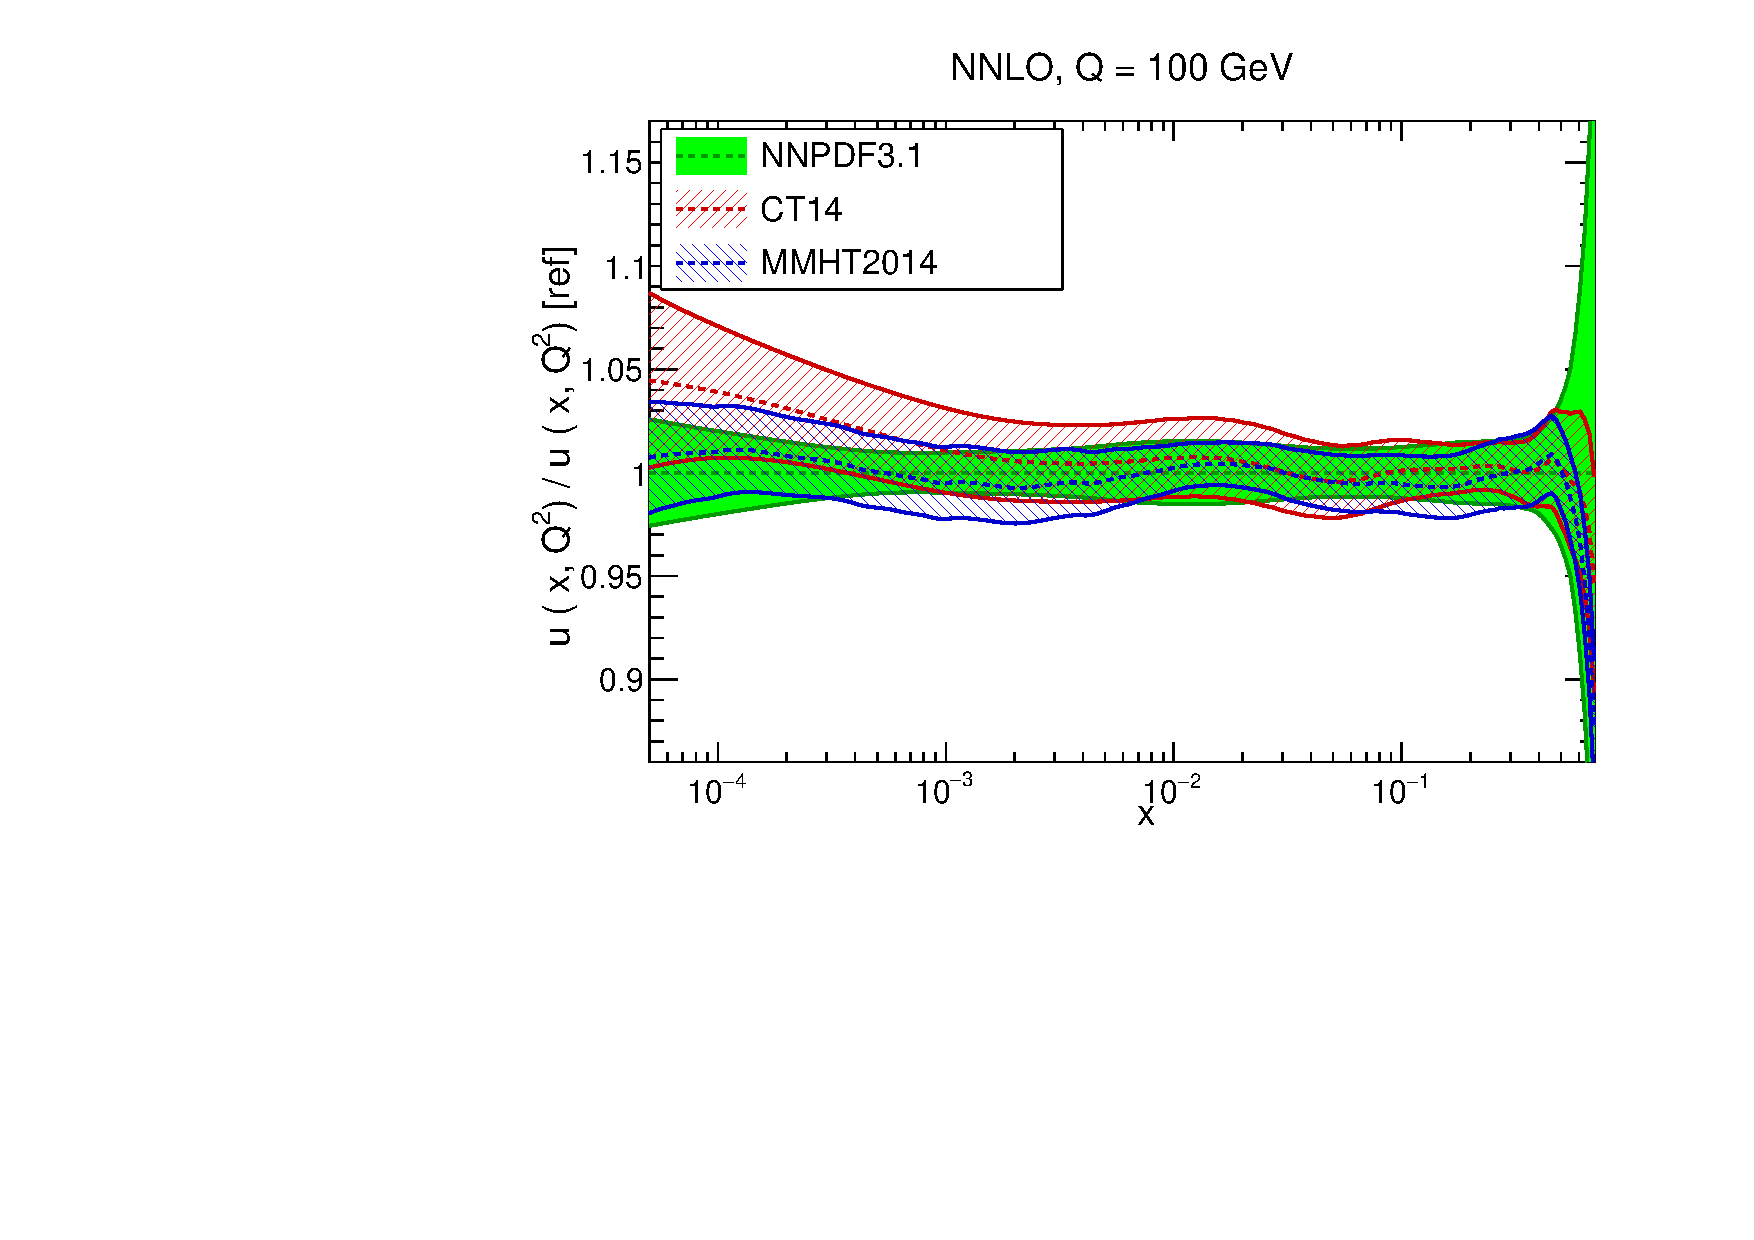
\includegraphics[scale=0.37]{plots/xu-31-nnlo-globalfits.pdf}
    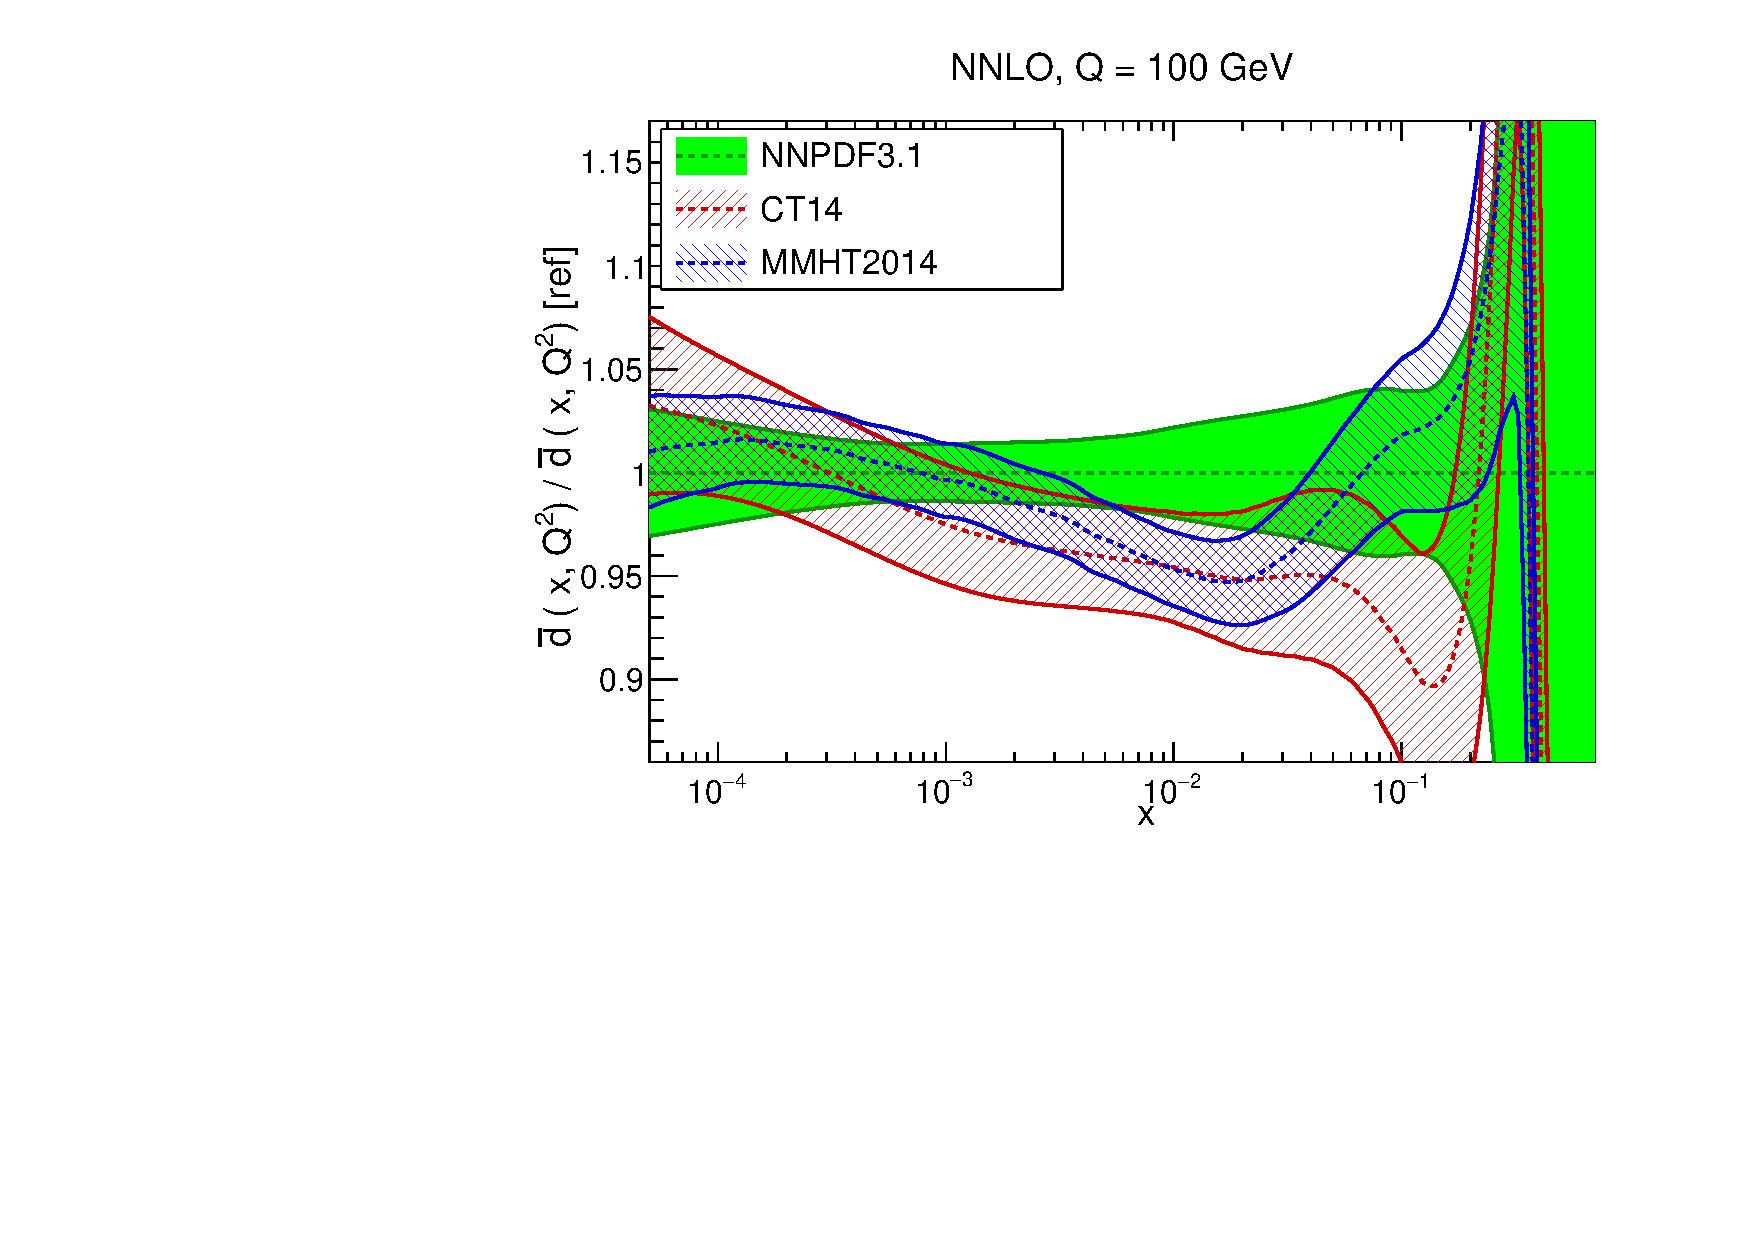
\includegraphics[scale=0.37]{plots/xdbar-31-nnlo-globalfits.pdf}
  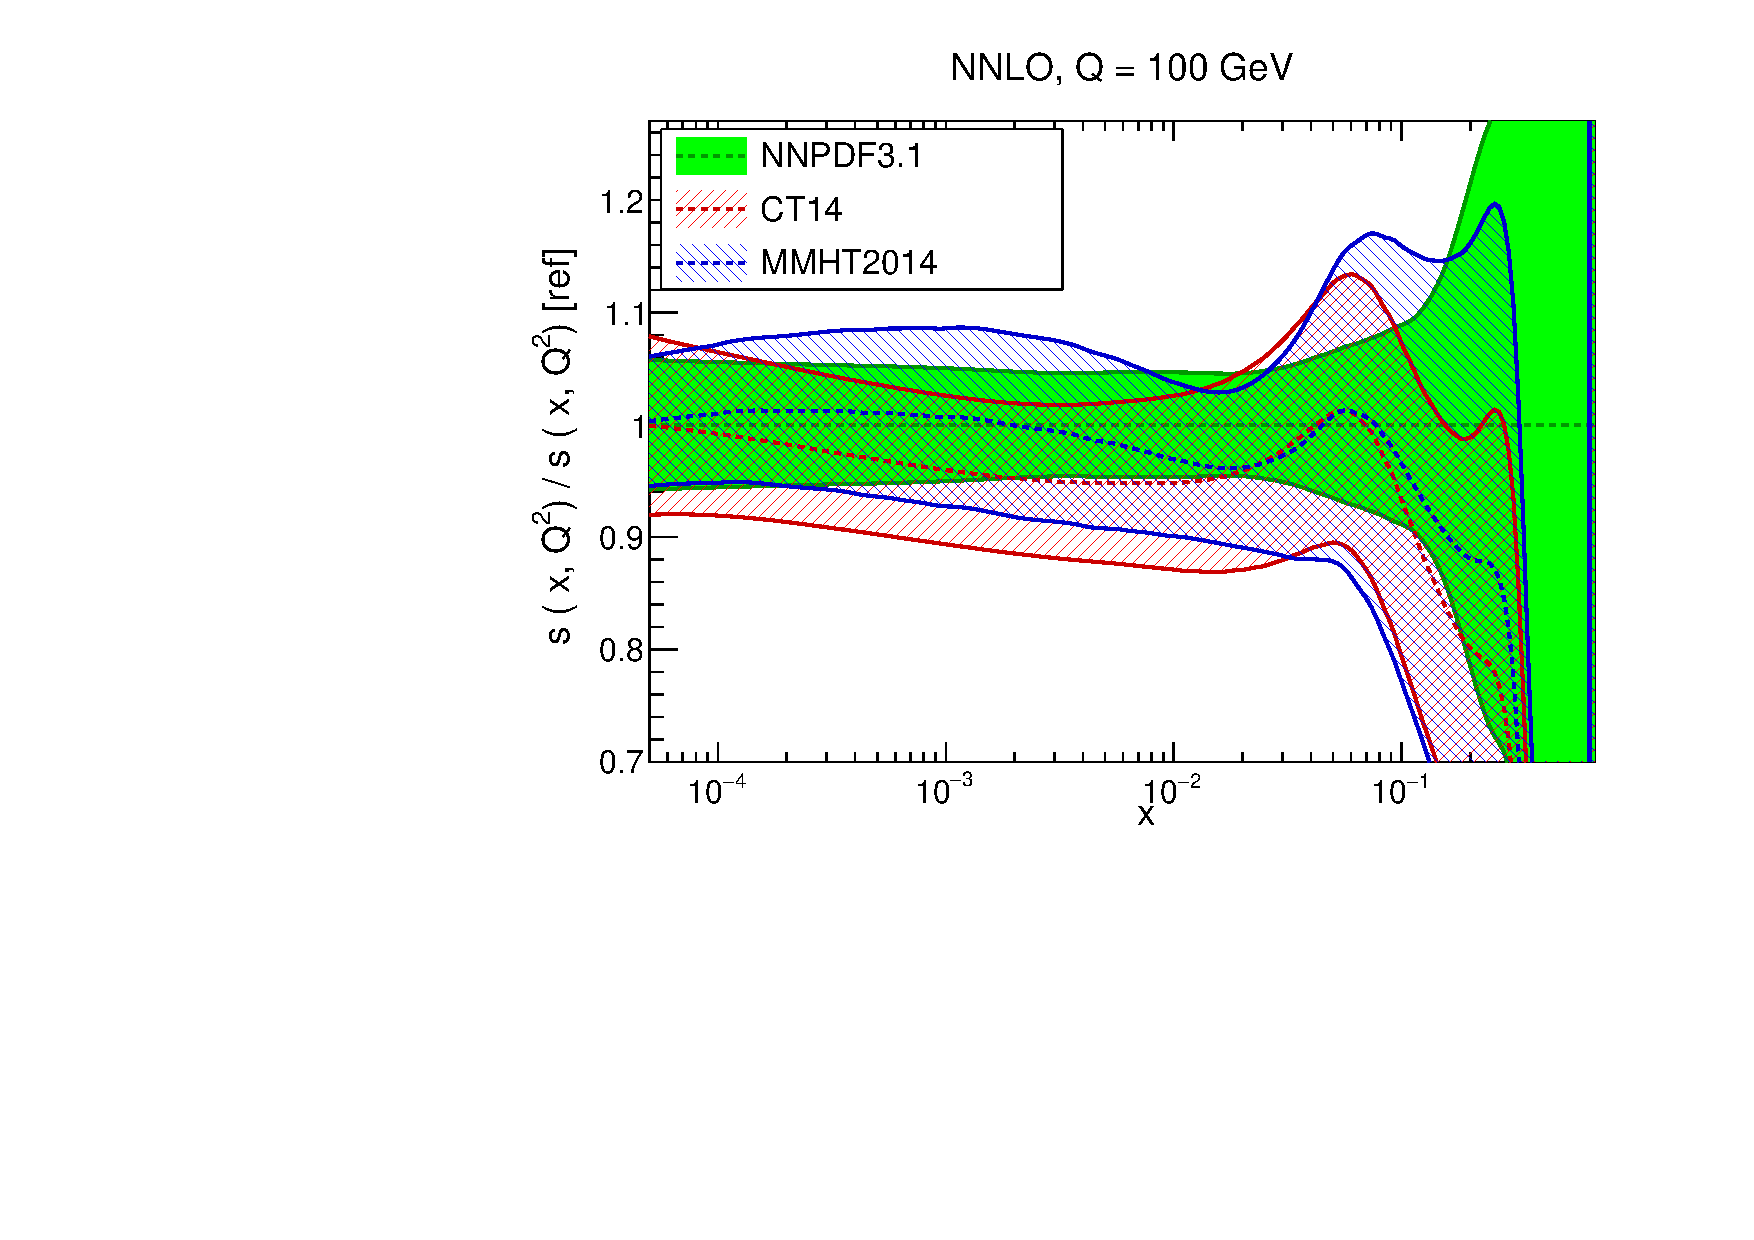
\includegraphics[scale=0.37]{plots/xs-31-nnlo-globalfits.pdf}
   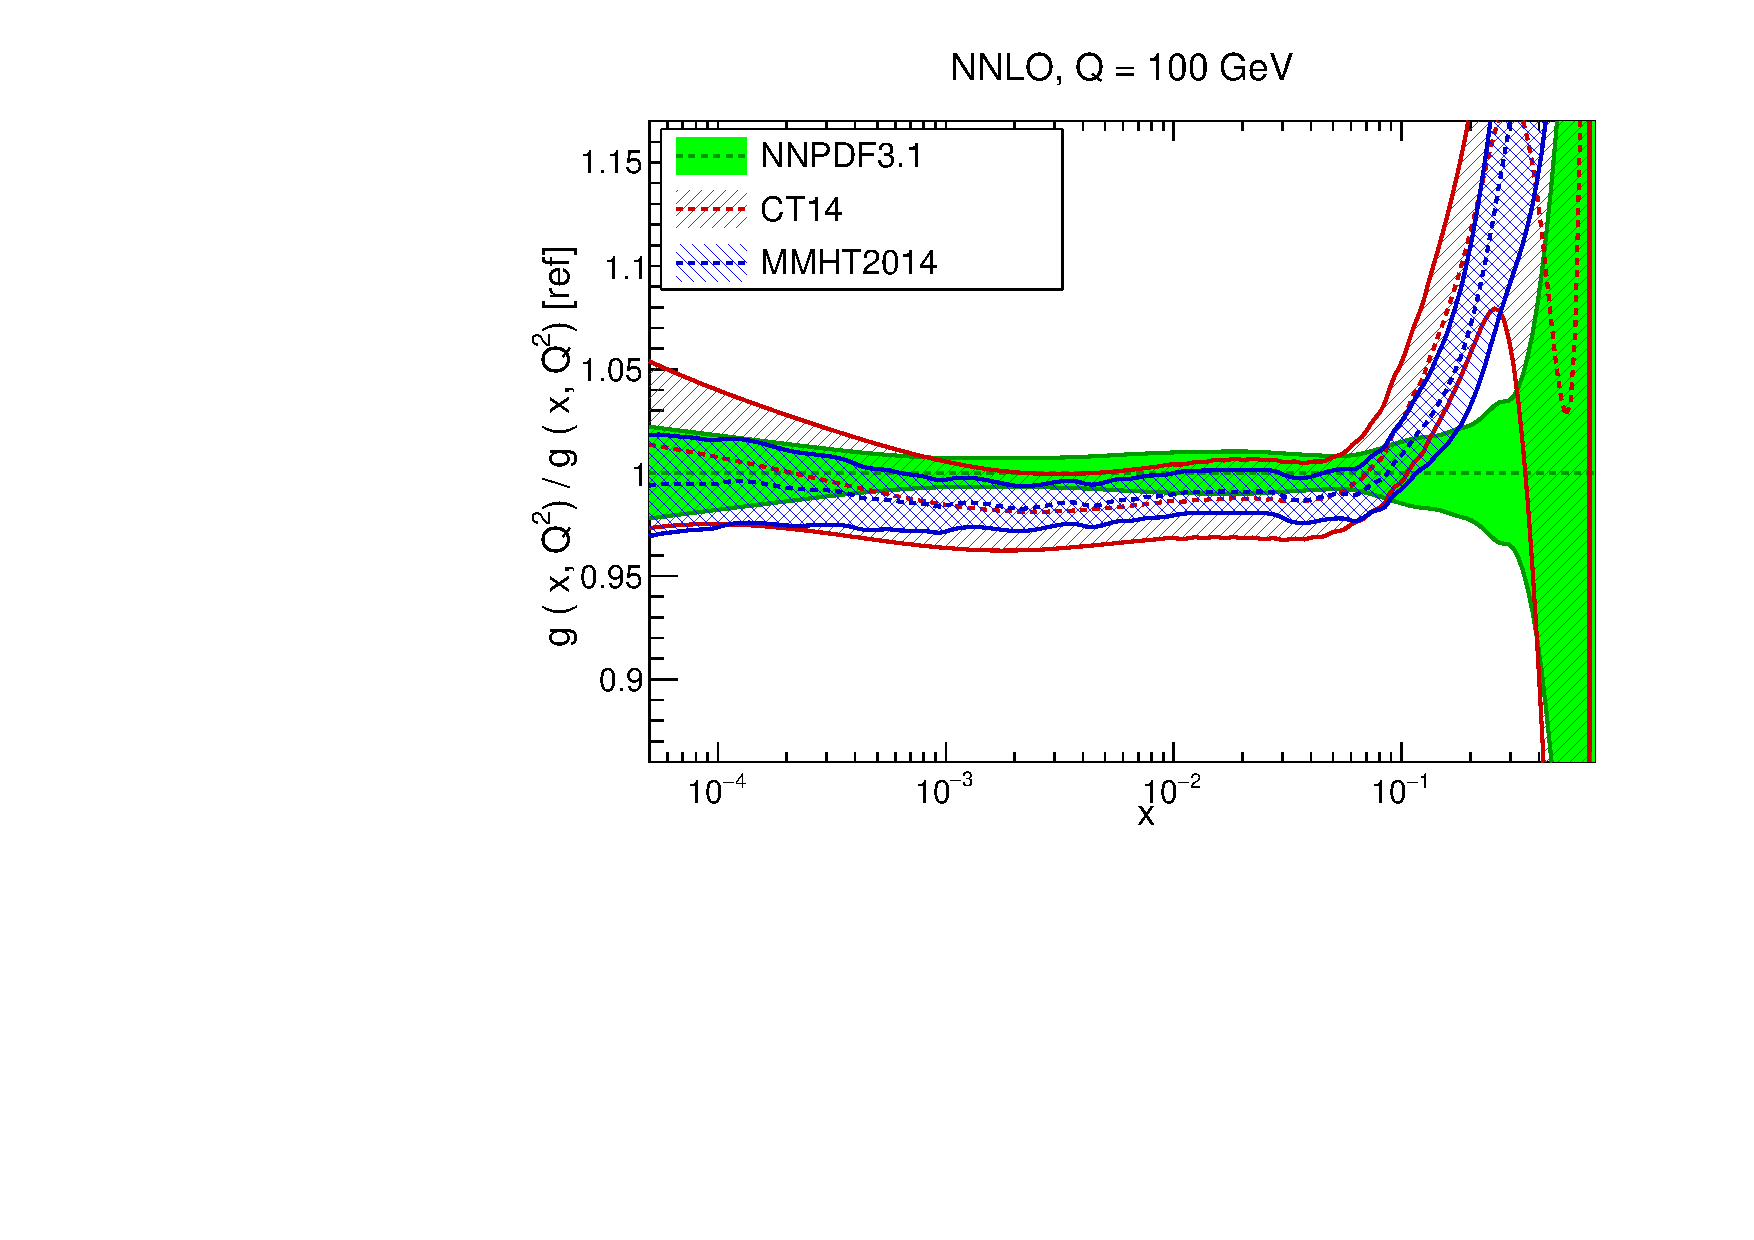
\includegraphics[scale=0.37]{plots/xg-31-nnlo-globalfits.pdf}
  \caption{\small Comparison between the CT14, MMHT2014
  and NNPDF3.1 NNLO PDF sets at $Q=100$ GeV, normalised
  to the central value of the latter.
  %
  From top to bottom and from left to right we show the
  $u$, $\bar{d}$ and $s$ quark PDFs as well as the gluon.
  %
  The error bands indicate the 1-$\sigma$ PDF uncertainties
  associated to each set.
  %
  These PDF comparison plots have been produced using the
  {\tt APFEL-Web} online plotting interface~\cite{Carrazza:2014gfa}.
    \label{fig:globalfits}
  }
\end{center}
\end{figure}
%%%%%%%%%%%%%%%%%%%%%%%%%%%%%%%%%%%%%%%%%%%%%%%%%%%%%%%%%%%%%%%%%%%%%%

In addition to these latest versions of the global PDF fits,
there has recently been a significant development of techniques aiming
to construct combined PDF sets that are based on
a small number of Hessian eigenvectors or MC replicas and thus
are more efficient to use in lengthy higher-order
computations or Monte Carlo simulations.
%
In particular, the PDF4LHC15 PDF sets are based on the
combination of the CT14, MMHT14 and NNPDF3.1 NNLO PDF sets,
subsequently reduced to a small number of eigenvectors
(replicas) using the META-PDF~\cite{Gao:2013bia}
and MC2H~\cite{Carrazza:2015aoa}
(CMC~\cite{Carrazza:2015hva}) compression algorithms.
%
In this respect, Specialized Minimal PDF sets~\cite{Carrazza:2016htc}
(SM-PDFs) have also
been advocated, which
are tailored to specific physical processes and are based
on the minimal number of Hessian eigenvectors.
%
The PDF4LHC15 sets provide a suitable representative for the expectations
from the global QCD analysis point of view, and as such will be used
in the benchmark comparisons of the next section.

Finally, and particularly relevant for the discussions in this white-paper,
we strongly encourage the community to use the most recent versions
of global PDF fits when comparing with existing or new
lattice QCD calculations.
%
Comparing with deprecated sets, based on obsolete methodology
and in many cases experimental data that has already been
superseded, should always be avoided.



\subsubsection{Polarised PDFs}
\label{sec:polPDFs}

Like their unpolarised (spin-averaged) counterparts described in the previous 
subsection, helicity PDFs, along with estimates of their uncertainties, can be 
determined from a comprehensive global analysis of the available spin-dependent 
data. 
%
Here we delineate the aspects of the framework specific to the polarised
case, and give a brief review of current global polarised PDF fits.

\paragraph{General framework.}
%
The dependence on the momentum fraction $x$, fixed by non-perturbative QCD 
dynamics, should satisfy some theoretical constraints.
%
First, PDFs must lead to positive cross sections.
At leading order (LO), this implies that polarised 
PDFs are bounded by their unpolarised counterparts\footnote{Beyond LO, more 
complicated relations hold~\cite{Altarelli:1998gn}; however they have little
effect on PDFs.}, $|\Delta f(x,\mu^2)|\leq f(x,\mu^2)$.
%
Second, PDFs must be integrable: this corresponds to the assumption 
that the nucleon matrix element of the axial current for each flavour is finite.
%
Third, SU(2) and SU(3) flavour symmetry, if assumed to be exact, imply that 
the first moments of the nonsinglet $\mathcal{C}$-even PDF combinations,
$\Delta T_3=\Delta u^+ -\Delta d^+$ and 
$\Delta T_8 = \Delta u^+ +\Delta d^+ -2\Delta s^+$ 
(where $\Delta q^+=\Delta q+\Delta\bar{q}$, $q=u,d,s$), are respectively
related to the baryon octet $\beta$-decay constants, whose 
measured values values are~\cite{Olive:2016xmw}
\begin{align}
 a_3
 & =
 \int_0^1 dx \Delta T_3 (x,\mu^2)
 = \langle 1\rangle_{\Delta u^+} - \langle 1\rangle_{\Delta d^+}  = 1.2701 \pm 0.0025
 ,,\\
 a_8
 & =
 \int_0^1 dx \Delta T_8 (x,\mu^2)
 = \langle 1 \rangle_{\Delta u^+} + \langle 1 \rangle_{\Delta d^+} -2\,\langle 1 \rangle_{\Delta s^+} 
 =0.585  \pm 0.025
 \,.
\label{eq:decayconst}
\end{align}
%
Fairly significant violations of SU(3) symmetry are advocated
in the literature (see {\it e.g.} Ref.~\cite{Cabibbo:2003cu} for a review). 
%
In this case, an uncertainty on the octet axial charge, larger by up to $30\%$ 
than its experimental value in Eq.~\eqref{eq:decayconst}, 
is found~\cite{FloresMendieta:1998ii}. 

The bulk of the experimental information on polarised PDFs comes from 
neutral-current (photon exchange) inclusive and semi-inclusive deep-inelastic scattering 
(DIS and SIDIS) with charged lepton beams and nuclear targets. 
%
As the photon scattering does not distinguish quarks and antiquarks, inclusive DIS 
data constrain only the total quark combinations $\Delta q^+$, 
while SIDIS data with identified pions or kaons in the final state 
constrain individual quark and antiquark flavours. 
%
In principle, both DIS and SIDIS are also sensitive to the gluon 
distribution $\Delta g$, as it directly enters the factorised expressions of
the corresponding structure functions beyond LO, and indirectly via DGLAP 
evolution.
%
In practice the constraining power of DIS and SIDIS data on $\Delta g$ is 
rather weak, because of the limited $Q^2$ range covered by the data. 

Note that, in the case of SIDIS, a reliable knowledge of fragmentation 
functions (FFs) is required in the factorised expressions of the 
corresponding observables. 
%
Since FFs are non-perturbative objects on the same footing as PDFs, they are 
an additional source of uncertainty in the PDF determination, and can  
even become a bias.
%
For this reason, a significant experimental and theoretical effort has been
invested in improving the independent determination of 
FFs~\cite{deFlorian:2014xna,deFlorian:2017lwf,
Hirai:2016loo,Sato:2016tuz,Nocera:2017qgb,Bertone:2017xsf,Ethier:2017zbq}.

Besides DIS and SIDIS fixed-target data, a significant amount of data from
longitudinally polarised proton-proton ($pp$) collisions at the Relativistic 
Heavy Ion Collider (RHIC) have become available recently (see {\it e.g.} 
Ref.~\cite{Aschenauer:2015eha} for an overview), although in a limited range 
of momentum fractions, $0.05\lesssim x \lesssim 0.4$.
%
On the one hand, longitudinal (parity-violating) single-spin and 
(parity-conserving) double-spin asymmetries for $W^\pm$ boson production are 
sensitive to the flavour decomposition of polarised quark and antiquark 
distributions, because of the chiral nature of the weak 
interactions~\cite{Bourrely:1993dd}. 
%
On the other hand, double-spin asymmetries for jet, di-jet and $\pi^0$ 
production are directly sensitive to the gluon polarisation in 
the proton, because of the dominance of gluon-gluon and quark-gluon initiated 
subprocesses in the kinematic range accessed by RHIC~\cite{Bourrely:1990pz}.

The kinematic coverage of the data that can be used to constrain polarised 
PDFs is displayed in Fig.~\ref{fig:kinEIC}.
%
A comparison with Fig.~\ref{fig:kinplot-report} makes it apparent that the
quantity of data points, their kinematic coverage and the variety of 
available hard-scattering processes are presently much more limited in the polarised case
than in the unpolarised case.
%
Therefore polarised PDFs can currently be determined with much less 
precision than their unpolarised counterparts and only over an $x$-range limited
to $x\gtrsim 0.005$.
%
The kinematic coverage is expected to be significantly extended in the future,
with DIS and SIDIS data from JLab-12~\cite{Dudek:2012vr} and a polarised 
high-energy Electron-Ion Collider (EIC)~\cite{Accardi:2012qut}.
%
Such an extended kinematic coverage is also displayed in Fig.\ref{fig:kinEIC}.
%
The eRHIC realisation of an EIC~\cite{Aschenauer:2014cki} has been considered.

%-------------------------------------------------------------------------------
\begin{figure}[!t]
\centering
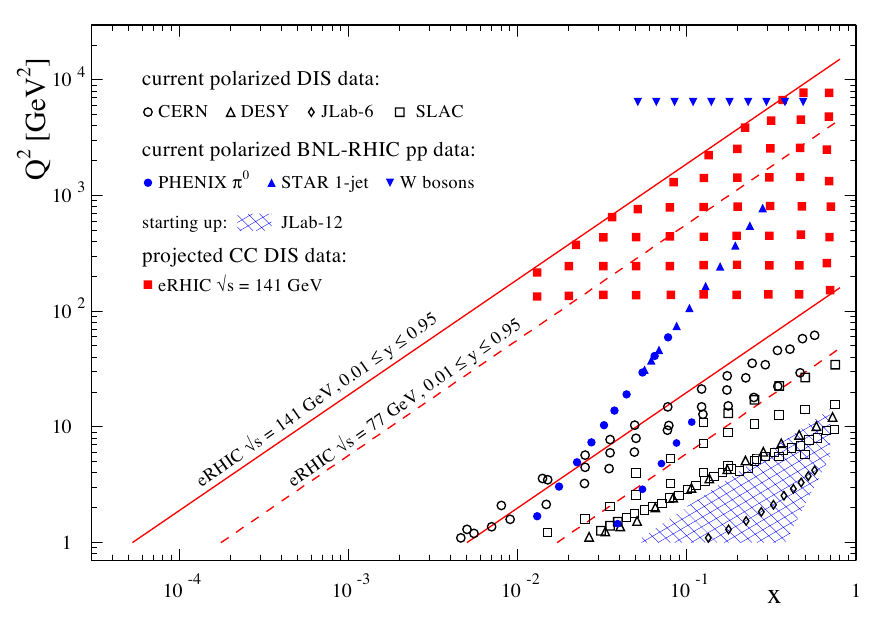
\includegraphics[width=0.9\textwidth]{plots/kinEIC}\\
\caption{\small Representative kinematic coverage, in the $(x,Q^2)$ plane,
of the (neutral current) DIS, SIDIS and $pp$ hard-scattering measurements 
that are used as input in a global polarised PDF fit.
%
The extended kinematic coverage achieved by 
JLab-12~\cite{Dudek:2012vr} and by the eRHIC~\cite{Aschenauer:2014cki} 
realisation of an EIC~\cite{Accardi:2012qut}
(including projected charged-current (CC) DIS data) is also shown.
%
Figure taken from Ref.~\cite{Aschenauer:2014cki}.}
\label{fig:kinEIC}
\end{figure}
%-------------------------------------------------------------------------------

A representative illustration of polarised PDFs obtained from a global
QCD analysis, namely NNDPFpol1.1~\cite{Nocera:2014gqa}, is provided in Fig.~\ref{fig:qPDFpol}.
%
The format is the same as for the unpolarised case, Fig.~\ref{fig:nnlopdfs},
in order to ease any comparison between the two.
%
In particular, note the suppression of all polarised PDFs at small values of 
$x$, including polarised sea quark PDFs, with respect to their unpolarised 
counterparts.

%-------------------------------------------------------------------------------
\begin{figure}[!t]
\centering
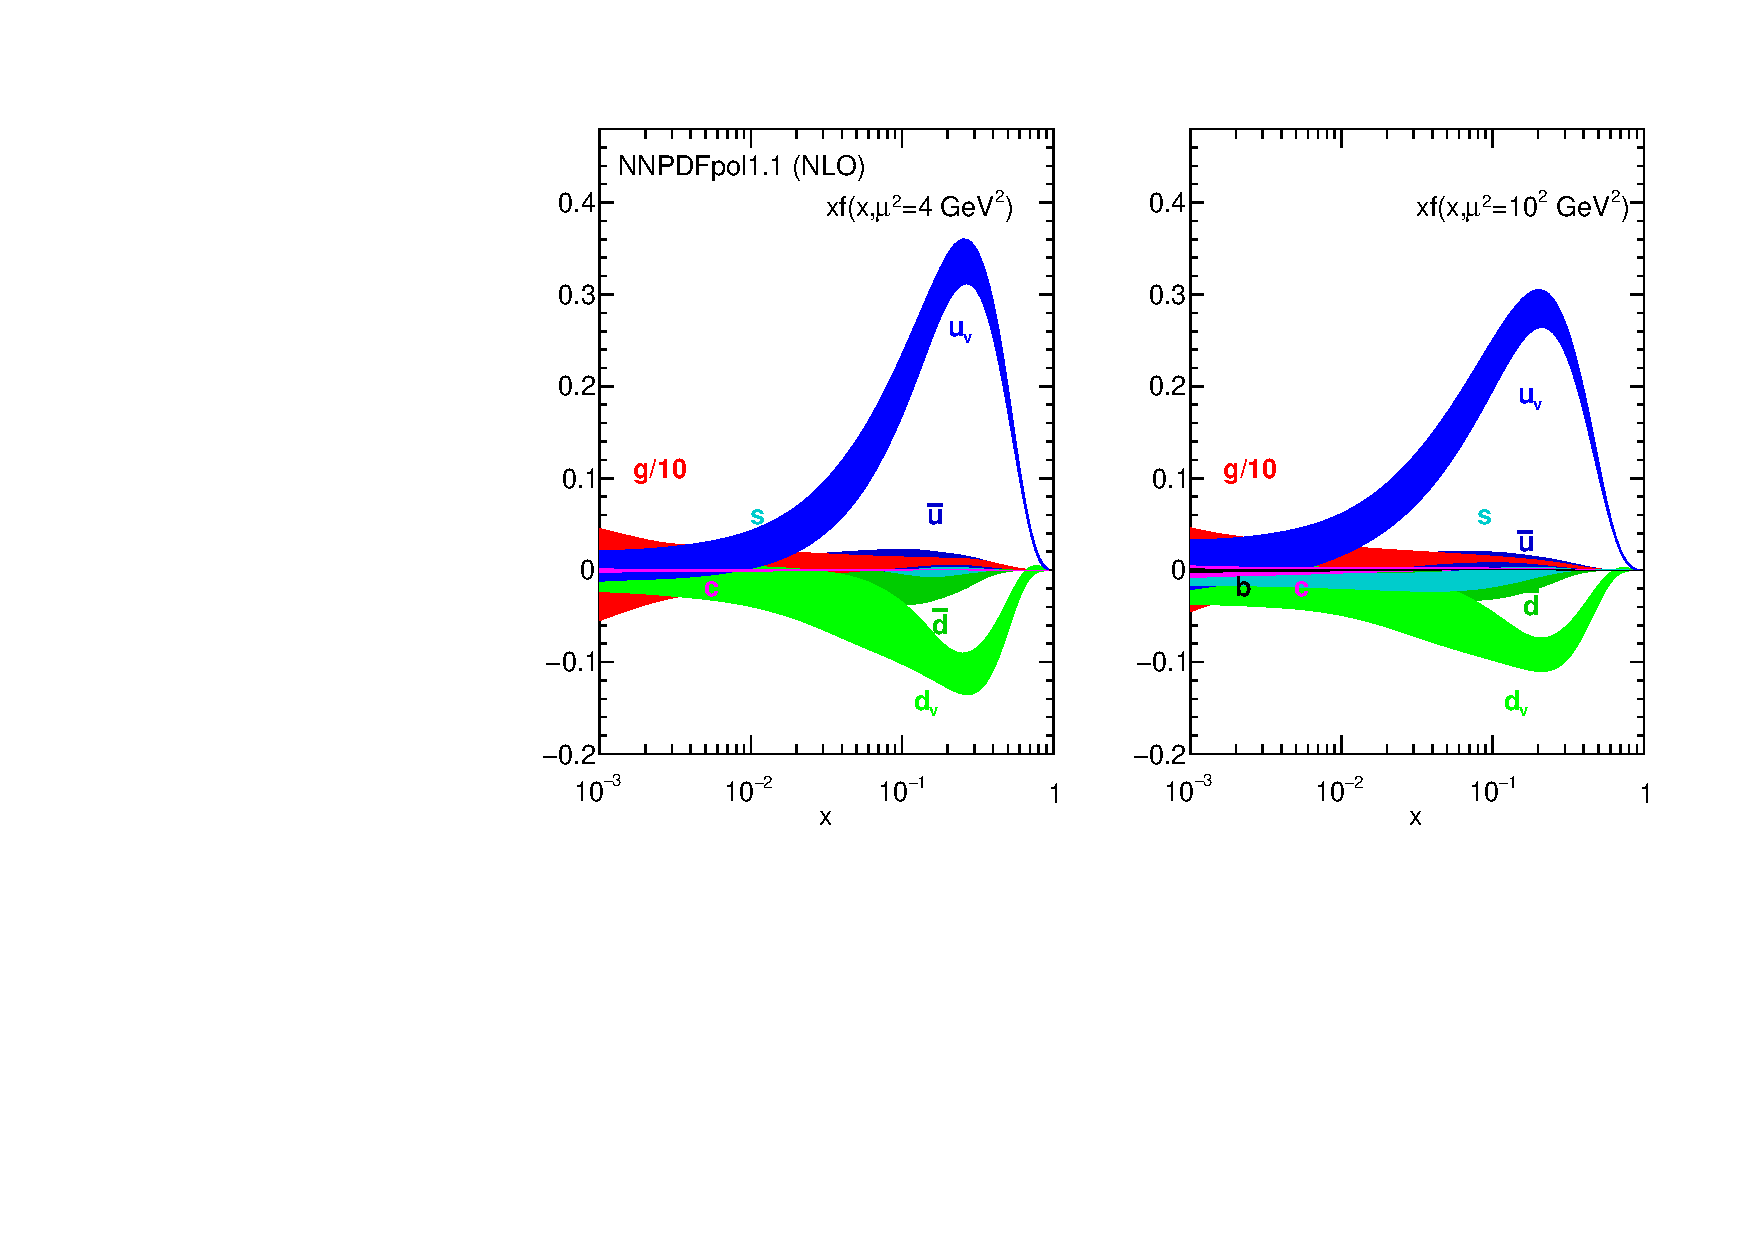
\includegraphics[scale=0.8]{plots/NNPDFpol11}\\
\caption{\small Same as Fig.~\ref{fig:nnlopdfs}, 
but for the polarised NNPDFpol1.1 NLO PDFs~\cite{Nocera:2014gqa}.}
\label{fig:qPDFpol}
\end{figure}
%-------------------------------------------------------------------------------

\paragraph{State-of-the-art global polarised PDF fits.}

Several modern determinations of polarised PDFs of the proton (up to 
NLO\footnote{A NNLO QCD analysis of polarised PDFs based on inclusive DIS
data only was performed in Refs.~\cite{Shahri:2016uzl,Khanpour:2017cha}.
Inclusive DIS is the only polarised process for which coefficient functions
are known up to NNLO (all others are known only up to NLO).} 
and mostly in the $\overline{\rm MS}$ factorisation scheme) are available in 
the literature~\cite{Nocera:2014gqa,Nocera:2016xhb,deFlorian:2014yva,deFlorian:2008mr,deFlorian:2009vb,Sato:2016tuz,Leader:2010rb,Blumlein:2010rn,Bourrely:2014uha,Hirai:2008aj}. 
%
A key goal of these is to also unveil the size (and uncertainty) of
$\Delta\Sigma$ and  $\Delta G$ in Eq.~\eqref{eq:moments}. 
%
The various determinations differ among each other in the data sets included 
in the analysis, in some details of the QCD analysis (like the treatment of 
higher-twist corrections) and in the procedure used to determine PDFs from the 
data (for details, see {\it e.g.} Chap.~3 in Refs.~\cite{Nocera:2014vla} 
and~\cite{Nocera:2016xhb}). 
%
The NNDPF procedure and the conventional/standard one adopted by DSSV have 
already been outlined in Sec.~\ref{sec:unpPDFs}. 
%
We note that DSSV has developed a method based on Mellin moments of the PDFs 
in order to efficiently incorporate NLO computations
of $pp$ cross sections in the fitting procedure. 
%
The JAM collaboration has implemented for their analysis a new approach called 
iterative Monte Carlo procedure~\cite{Sato:2016tuz}. 

Motivated by the interest in assessing the impact of RHIC $pp$ 
data, two new global analyses of polarised PDFs have been carried out in
2014, DSSV14~\cite{deFlorian:2014yva} and NNPDFpol1.1~\cite{Nocera:2014gqa}.
%
They upgrade the corresponding previous analyses, 
DSSV08~\cite{deFlorian:2008mr,deFlorian:2009vb} and 
NNPDFpol1.0~\cite{Ball:2013lla}, with data respectively on double-spin 
asymmetries for inclusive jet production~\cite{Adamczyk:2014ozi} 
and $\pi^0$ production~\cite{Adare:2014hsq}\footnote{Preliminary RHIC results 
included in Ref.~\cite{deFlorian:2008mr} were replaced in
Ref.~\cite{deFlorian:2014yva} with final results.}, 
and on double-spin asymmetries for high-$p_T$ inclusive jet 
production~\cite{Adamczyk:2014ozi,Adamczyk:2012qj,Adare:2010cc} and single-spin
asymmetries for $W^\pm$ production~\cite{Adamczyk:2014xyw}.
%
The new data have been included in NNPDFpol1.1 
by means of Bayesian reweighting~\cite{Ball:2010gb},
and in DSSV14 by means of a full refit.  

Overall, both the DSSV14 and NNPDFpol1.1 PDF determinations are 
state-of-the-art in the inclusion of the available experimental information. 
%
The data sets in the two analyses differ between each other only in
fixed-target SIDIS and RHIC $\pi^0$ production measurements, included in 
DSSV14, but not in NNPDFpol1.1. 
%
The information brought in by these data is complementary to that provided by 
RHIC $W^\pm$ production and inclusive jet production data respectively,
although fraught with larger theoretical uncertainties related to fragmentation.

%------------------------------------------------------------------------------
\begin{figure}[!t]
%\centering

\hspace*{6mm}
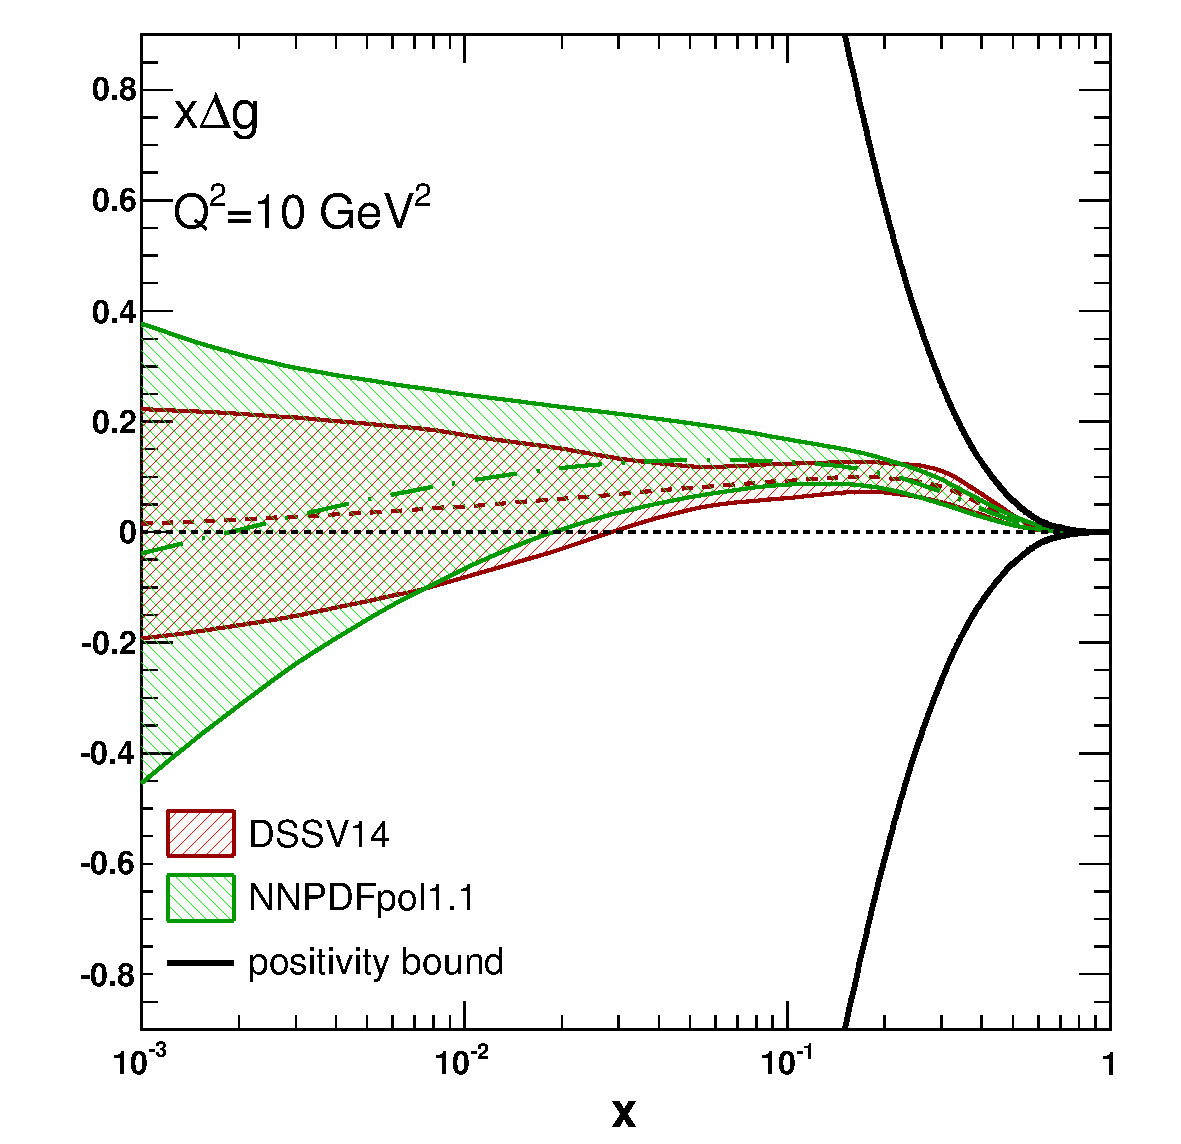
\includegraphics[scale=0.325]{plots/gluoncomp}

\vspace*{-15.1cm}
\hspace*{8cm}
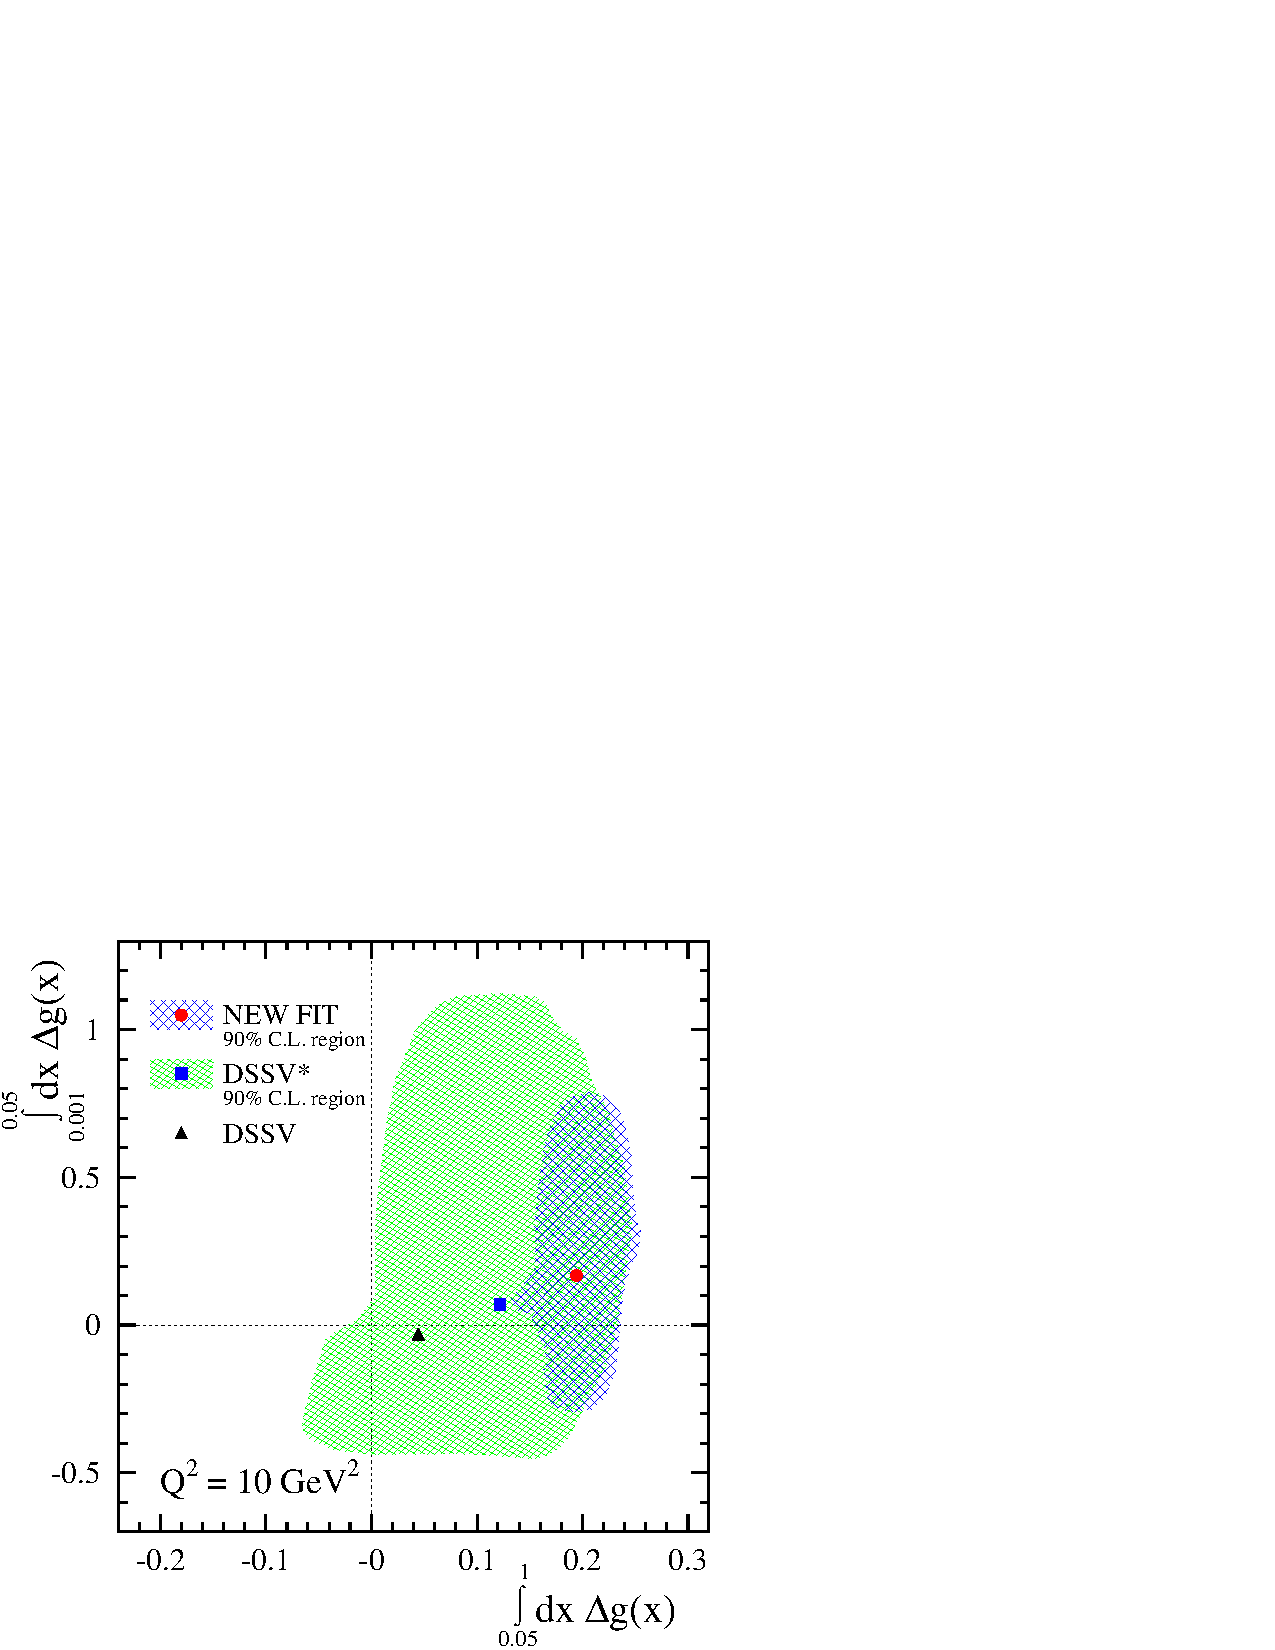
\includegraphics[scale=0.555]{plots/correlation_getot.pdf}

\caption{\small (Left) The polarised gluon momentum distribution  
$x\Delta g$ from the DSSV14 (with $90\%$ C.L. uncertainty band)
and NNPDFpol1.1 PDF sets at $Q^2=10$ GeV$^2$. The NNPDF3.1 positivity
bound is also shown.
(Right) $90\%$ C.L.\ areas in the plane spanned by the truncated moments of
$\Delta g$ computed for $0.05\leq x\leq 1$ and $0.001\leq x\leq 0.05$ at $Q^2=10\,\mathrm{GeV}^2$~\cite{deFlorian:2014yva}.}
\label{fig:RHICpdfs}
\end{figure}
%------------------------------------------------------------------------------

The effect of RHIC data on the polarised PDFs of the proton is twofold:
\begin{itemize}

\item The 2009 STAR and PHENIX data sets on jet and $\pi^0$ 
production~\cite{Adamczyk:2014ozi,Adare:2014hsq}, included in DSSV14
and NNPDFpol1.1, provide the first evidence
of a sizable positive gluon polarisation in the proton. 
%
A comparison of the gluon PDF in the two PDF sets is displayed in 
Fig.~\ref{fig:RHICpdfs} (left panel). 
%
Comparable results, both central values and uncertainties, are found in the 
$x$ region covered by RHIC data. 
%
The agreement between the two analyses is optimal in the
range $0.08\leq x \leq 0.2$, where the dominant experimental information comes
from jet data; a slightly smaller central value is found in the DSSV14 
analysis, in comparison to the NNPDFpol1.1, in the range 
$0.05\leq x \leq 0.08$, where the dominant experimental information comes from 
$\pi^0$ production data. 
%
Indeed, these are included in DSSV14 but are not
in NNPDFpol1.1. 
%
Nevertheless, best fits lie well within each other error
bands, though NNPDFpol1.1 uncertainties tend to be larger than DSSV14
uncertainties outside the region covered by RHIC data.
%
Very consistent values of the integral of $\Delta g$, 
Eq.~\eqref{eq:moments}, truncated over the interval $0.05\leq x \leq 1$, are 
found: at $Q^2=10$ GeV$^2$, this is $0.20^{+0.06}_{-0.07}$ for 
DSSV14~\cite{deFlorian:2014yva}, and $0.23\pm 0.06$ for 
NNPDFpol1.1~\cite{Nocera:2014gqa}. The right plot in Fig.~\ref{fig:RHICpdfs} 
shows the corresponding DSSV14 result as an example; the impact of the RHIC
data is clearly visible. 

\item The 2012 STAR data sets on $W$ production~\cite{Adamczyk:2014xyw}, 
included in NNPDFpol1.1, provide evidence of a positive 
$\Delta\bar{u}$ distribution 
and a negative $\Delta\bar{d}$ distribution, with 
$|\Delta\bar{d}|>|\Delta\bar{u}|$~\cite{Nocera:2014gqa},
as shown in Fig.~\ref{fig:RHICpdfs1}.
% 
The size of the flavour symmetry breaking for polarised sea quarks is 
quantified by the asymmetry $\Delta\bar{u}-\Delta\bar{d}$, which,
in the NNPDFpol1.1 analysis, turned out to be roughly as large as its 
unpolarised counterpart (in absolute value), 
though much more uncertain~\cite{Nocera:2014rea}. 
%
Even within this uncertainty, polarised and unpolarised light sea quark 
asymmetries show opposite signs,
with the polarised ones being clearly positive.  This trend is also found
from analysis of the polarised SIDIS data, as revealed by the DSSV analyses. 
%
This result may discriminate among models of nucleon structure; 
see Fig.~\ref{fig:RHICpdfs1}: 
specifically, some meson-cloud (MC) models are disfavored, while a more 
accurate experimental information is needed to establish whether 
chiral quark-soliton (CQS), Pauli-blocking (PB) or statistical (ST)
models are preferred (all these models are described in 
Ref.~\cite{Chang:2014jba}).

\end{itemize}

%------------------------------------------------------------------------------
\begin{figure}[!h]
\centering
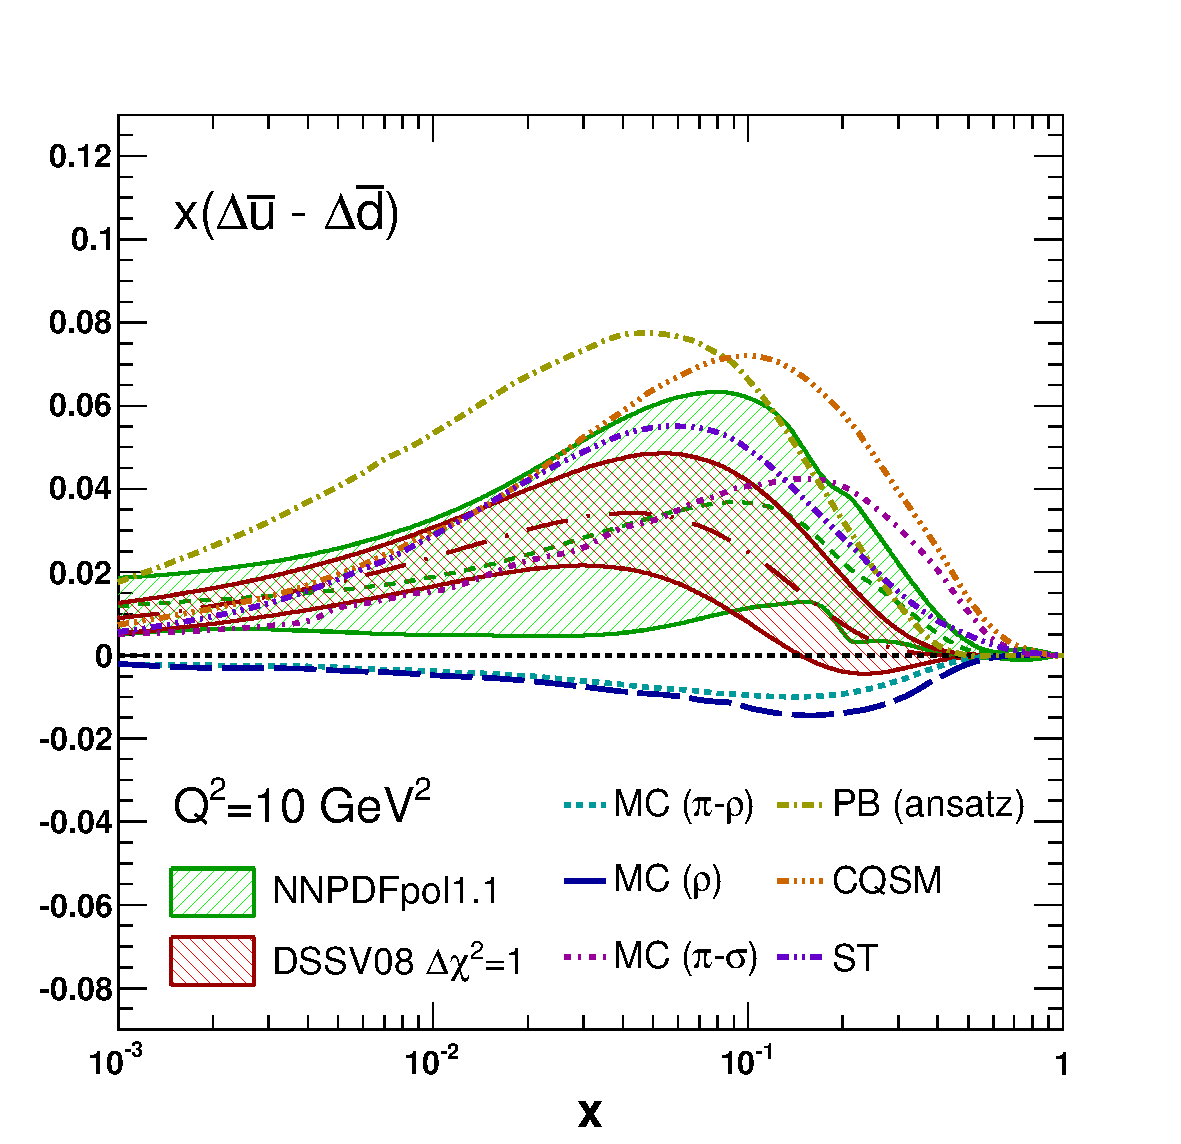
\includegraphics[scale=0.35]{plots/asysea_2}\\
\caption{\small The polarised light sea quark asymmetry 
$x(\Delta\bar{u}-\Delta\bar{d})$ from the NNPDFpol1.1 and 
DSSV08 PDF sets at $Q^2=10$ GeV$^2$, compared to expectations from 
various models of nucleon structure~\cite{Chang:2014jba}.}
\label{fig:RHICpdfs1}
\end{figure}
%------------------------------------------------------------------------------

\paragraph{Open issues.}

Despite the achievements described above, the polarised PDFs presently cannot 
be determined in a global QCD analysis with the same accuracy as their 
unpolarised counterparts.
%
The experimental data are confined to a relatively narrow range of 
$x$ and $Q^2$.
%
As a consequence, the sizes of the contribution of quarks, antiquarks and 
gluons to the nucleon spin, as quantified by their first moments, 
Eq.~\eqref{eq:moments}, are still affected by large uncertainties. 
%
These come predominantly from the extrapolation into the small-$x$ region 
($x\lesssim 10^{-3}$). 
%
Here potential modifications in the PDF shape induced by small-$x$ evolution 
could arise, which presently cannot be tested.
%
Significant uncertainties also affect the PDFs in the large-$x$ 
{\it valence} region ($x\gtrsim 0.7$). 
%
This regime is less relevant for determination of the first moments, but is 
important for comparisons to nonperturbative models of nucleon structure, 
especially in terms of ratios of light-quark polarised to unpolarised PDFs 
(for a comparison between large-$x$ PDFs 
and model predictions, see Ref.~\cite{Nocera:2014uea}).
%
Finally, the small lever arm of the data in $Q^2$ is a serious limiting factor 
in the determination of $\Delta g$ via evolution and the assessment of possible 
higher-twist contributions. 

The determination of the total polarised strange distribution $\Delta s^+$ is 
also particularly delicate.
%
Inclusive DIS data, together with nonsinglet axial couplings, 
Eq.~\eqref{eq:decayconst}, and kaon SIDIS data provide the sole available 
constraint on $\Delta s^+$.
%
A sizeable negative $\Delta s^+$ is found 
consistently in all analyses based on inclusive DIS data only, as a result 
of the constraint from hyperon decays that is usually adopted. 
%
However, the shape of $\Delta s^+$ may change significantly in analyses that also include
SIDIS data. Typically SIDIS data lead to a trend for $\Delta s^+$ to be
small or even slightly positive in the medium $x$-range, although this depends 
also on the set of kaon FFs used to compute
the corresponding observables~\cite{Leader:2011tm}.  
%
The recent study in Ref.~\cite{Ethier:2017zbq} sheds some light on this issue
by performing a simultaneous determination of polarised PDFs and unpolarised 
fragmentation functions using DIS, SIDIS and single-inclusive annihilation data.
%
In order to avoid biasing the determination of $\Delta s^+$ by 
assumptions on SU(3) symmetry, the octet axial charge in 
Eq.~\eqref{eq:decayconst} has been allowed to be determined by the data alone.
%
As a consequence, a slightly positive $\Delta s^+$ distribution, but
compatible with the negative result found from inclusive DIS within its 
large uncertainties, has been obtained.
% 
An octet axial charge about $20\%$ smaller than its quoted experimental value, 
Eq.~\eqref{eq:decayconst} appears to be preferred by the data.
%
However, we stress that the determination of $\Delta s^+$ from SIDIS data 
also relies on good knowledge of the {\it un}polarised strange distribution. 
%
Furthermore, unpolarised SIDIS data themselves set constraints on 
fragmentation functions and ultimately would need to be included as well
in order to obtain a reliable picture. 
%
In any case, further higher precision kaon SIDIS data will be needed in order 
to reduce the uncertainty on $\Delta s^+$ and further test the degree of 
SU(3) breaking. 

Ongoing and future experimental campaigns at current facilities are
expected to provide additional experimental information
useful to clarify some of the issues outlined above (for an 
assessment of the impact of very recent/forthcoming data, see {\it e.g.}
Refs.~\cite{Aschenauer:2015eha,Aschenauer:2015ata,Nocera:2015vva,
Nocera:2017wep}).
%
However, a future high-energy, polarised EIC~\cite{Accardi:2012qut} will 
likely be the only facility to be able to address all the above issues 
with the highest precision. 
% 
The extension of the kinematic reach down to $x\sim 10^{-4}$ and up to
$Q^2=10^4$ GeV$^2$ will allow for an accurate determination of $\Delta g$
via evolution in DIS/SIDIS, of $\Delta\bar{u}$ and 
$\Delta\bar{d}$ via inclusive DIS at high $Q^2$ mediated by electroweak bosons,
and of $\Delta s$ via kaon-tagged SIDIS. 
%
The potential impact of the longitudinally polarised program at an EIC
has been quantitatively assessed in several dedicated 
studies~\cite{Aschenauer:2012ve,Ball:2013tyh,Aschenauer:2013iia,
Aschenauer:2015ata}.



%%%%%%%%%%%%%%%%%%%%%%%%%%%%%%%%%%%%%%%%%%%%%%%%%%%%%%%%%%%%%%%%%%%%%%%%%%%%%%%%
\section{Benchmarks}
\label{sec:benchmarking}
%%%%%%%%%%%%%%%%%%%%%%%%%%%%%%%%%%%%%%%%%%%%%%%%%%%%%%%%%%%%%%%%%%%%%%%%%%%%%%%%

The aim of this section is to provide a quantitative comparison between 
current lattice-QCD and global-PDF fit results.
%
To this purpose, we shall identify the appropriate benchmark quantities, 
and define the criteria to carefully appraise the corresponding determinations
available in the literature.
%
For each benchmark quantity, we shall specify the prescription adopted to 
select and combine, on the one hand, lattice-QCD calculations, and, on the 
other hand, global PDF-fit determinations.
%
We finally present our benchmark numbers from each side and compare them.

%%%%%%%%%%%%%%%%%%%%%%%%%%%%%%%%%%%%%%%%%%%%%%%%%%%%%%%%%%%%%%%%%%%%%%%%%%%%%%%%
\subsection{Benchmark criteria}
\label{subsec:BC}

We start by describing our benchmark criteria, which include the definition
of the benchmark quantities and the determination of their reference values,
based on a careful assessment of the lattice-QCD and global-PDF results 
available in the literature.

\subsubsection{Benchmark quantities}
\label{subsubsec:BQ}

We identify our benchmark quantities with the lowest moments of unpolarised 
and polarised PDFs, or of some of their combinations, specifically: 
$\langle x\rangle_{u^+-d^+}$, $\langle x \rangle_{u^+}$, $\langle x \rangle_{d^+}$, 
$\langle x \rangle_{s^+}$ and $\langle x \rangle_{g}$ (in the unpolarised case); 
$g_A\equiv\langle 1 \rangle_{\Delta u^+ - \Delta d ^+}$, 
$\langle 1 \rangle_{\Delta u^+}$, $\langle 1 \rangle_{\Delta d^+}$,  
$\langle 1 \rangle_{\Delta s^+}$ and $\langle x \rangle_{\Delta u^- - \Delta d^-}$ 
(in the polarised case).
%
We use the notation outlined in Appendix~\ref{app:notation}.
%
The focus on these quantities is motivated by the fact that
current lattice calculations of higher moments and/or of other PDFs or PDF 
combinations are not sufficiently controlled to allow for a meaningful 
comparison between lattice-QCD and global-PDF fit results.
%
Therefore, these will not be considered here. 

\subsubsection{Appraising lattice-QCD calculations}
\label{subsubsec:BClQCD}

To accurately assess the current state-of-the-art for lattice calculations
available in the literature, we follow a procedure inspired by the review of 
low-energy mesons undertaken by the Flavor Lattice Averaging Group 
(FLAG)~\cite{Aoki:2016frl}. 
%
For each lattice calculation, we assess the status of each source of 
uncertainty outlined in Sec.~\ref{Sec:IntroLQCD}. 
%
We use a rating system inspired by FLAG, awarding a blue star (\bstar) for 
sources of uncertainty that are well-controlled or very conservatively 
estimated, a blue circle (\bcirc) for sources of uncertainty that have been 
controlled or estimated to some extent, and a red square (\rsquare) for 
uncertainties that have not met our criteria or for which no estimate is given.
%
Specifically, the rating system works as follows.

\begin{itemize}
\item {\bfseries Discretisation effects and the continuum limit.} 
We assume that the lattice actions are ${\cal O}(a)$-improved, {\it i.e.}, 
that the discretization errors vanish quadratically with the lattice spacing. 
%
For unimproved actions an additional lattice spacing is required. 
%
We require that these criteria are satisfied in each case for at least one 
pion mass below 300 MeV.
%
\begin{itemize}
%
\item[\bstar] At least three lattice spacings with at least two lattice 
spacings below 0.1 fm and a range of lattice spacings that satisfies 
$[a_{\mathrm{max}}/a_{\mathrm{min}}]^2 \geq 2$.
%
\item[\bcirc] At least two lattice spacings with at least one point below 
0.1 fm and a range of lattice spacings that satisfies 
$[a_{\mathrm{max}}/a_{\mathrm{min}}]^2 \geq 1.4$.
%
\end{itemize}
%
To receive a \bstar~or \bcirc~either a continuum extrapolation must be 
performed or the results must demonstrate no significant discretisation 
effects over the appropriate range of lattice spacings.

\item {\bfseries Unphysical pion masses.} 
For the following criteria, we define a physical pion mass ensemble 
to be one with $M_\pi=135\pm 10$~MeV.
%
\begin{itemize}
\item[\bstar] One ensemble with a physical pion mass \emph{or} a chiral 
extrapolation with three or more pion masses, with at least two pion masses 
below 250 MeV and at least one below 200~MeV.
%
\item[\bcirc] A chiral extrapolation with three or more pion mass, two of 
which are below 300~MeV.
%
\end{itemize}

\item {\bfseries Finite volume effects.} 
%
For calculations that use a mixed action approach, {\it i.e.},
with different lattice actions for the valence and sea quarks, 
we apply the criteria for $M_\pi L$ to the valence quarks.
%
\begin{itemize}
%
\item[\bstar] Ensembles with $M_{\pi,\mathrm{min}}L\geq 4$, \emph{or} at least 
three volumes with spatial extent $L>2.5$~fm.
\item[\bcirc] Ensembles with $M_{\pi,\mathrm{min}}L \geq 3.4$, \emph{or} at least 
two volumes with spatial extent $L>2.5$~fm.
\end{itemize}

\item {\bfseries Excited state contamination.} 
The following criteria must be satisfied for every pion mass and lattice 
spacing.
%
\begin{itemize}
%
\item[\bstar] At least three source-sink separations or a variational method 
to optimise the operator derived from at least a $3\times 3$ correlator matrix.
% 
\item[\bcirc] Two source-sink separations at every pion mass and lattice 
spacing, or three or more source-sink separations at one pion mass below 
300~MeV. 
%
For the variational method, an optimised operator derived from a $2\times 2$ 
correlator matrix at every pion mass and lattice spacing, or a $3\times 3$ 
correlator matrix for two pion masses below 300 MeV.
%
\end{itemize}

\item {\bfseries Renormalization.} 
\begin{itemize}
%
\item[\bstar] Nonperturbative renormalisation.
%
\item[\bcirc] Perturbative renormalisation.
%
\end{itemize}
%
For $g_A$ we also award a \bstar~for calculations that use fermion actions 
for which $Z_A/Z_V=1$ or employ combinations of quantities for which the 
renormalisation is unity by construction.

\item {\bfseries Lattice-spacing determination.} 
For lattice-QCD calculations of nucleons, the lattice-spacing determination is 
generally sufficiently precise that it is a very small or negligible source
of systematic uncertainty. 
%
Therefore we do not include an assessment of the lattice-spacing
determination in our criteria.

\end{itemize}

We now turn to summarise the current status of lattice-QCD calculations of
the first moments of unpolarised and polarised PDFs respectively.
%
Following FLAG, we consider only those results that are published in 
peer-reviewed journals or that have appeared as preprints. 
%
Where recent results are a clear update of previously published work, we do 
not include the earlier results.
%
A bibliographical compilation of the results available in the literature 
is given for completeness in 
Tabs.~\ref{tab:latticebibfirst}-\ref{tab:latticebiblast} 
of Appendix~\ref{sec:LQCDtables}.
%
We characterise the state-of-the-art results according to the criteria 
described above, and provide a prescription to combine those which satisfy 
them into a single benchmark value.

We remark that our criteria, and the corresponding ratings, are chosen 
not only to provide as fair an assessment of the relative merits of various 
calculations as possible, but to be aspirational. 
%
Where lattice-QCD results do not meet these standards, we hope that the lattice 
community will work towards improved calculations and greater precision as 
part of a concerted and inter-disciplinary effort to better understand
nucleon structure.

\paragraph{Unpolarised parton distributions.}
We summarise the current status of lattice-QCD calculations of the benchmark 
moments of unpolarised PDFs listed in Sec.~\ref{subsubsec:BQ} in 
Tab.~\ref{tab:unpolLQCDstatus1}. 
%
In the first column we indicate the computed moment, in the second column
the collaboration who performed the computation and in the third column
the corresponding reference.
%
In the fourth column we indicate the number of sea quark flavours, $N_f$, 
and in the fifth column we show whether the calculation has been published (P) 
or has appeared as a preprint (PreP).
%
In the following five columns we assess each source of systematic uncertainty
according to the criteria listed above. 
%
In the last column, we report the computed value at $\mu^2=Q^2=4$ GeV$^2$.
%
We indicate in parentheses the 68\% confidence level (CL) statistic uncertainty 
and the total systematic uncertainty respectively.
%
We do not list results that have not been extrapolated to the physical pion 
mass, nor do we include quenched results in Tab.~\ref{tab:unpolLQCDstatus1}. 
%
For completeness, we report these results in Tab.~\ref{tab:unpolLQCDstatus1B} 
of Appendix~\ref{sec:LQCDtables}.

%-------------------------------------------------------------------------------
\begin{table}[t] 
\renewcommand{\arraystretch}{1.2} 
\centering 
\begin{threeparttable}
\begin{tabular}{llcllccccccl}
Mom. & Collab. & Ref. & $N_f$ & Status & 
\begin{rotate}{70}{discretisation}\end{rotate} &
\begin{rotate}{70}{quark mass}\end{rotate} &
\begin{rotate}{70}{finite volume}\end{rotate} &
\begin{rotate}{70}{renormalisation}\end{rotate} &
\begin{rotate}{70}{excited states}\end{rotate}&
& Value\\
\toprule
$\langle x\rangle_{u^+-d^+}$ 
& LHPC\,14  
  & \cite{Green:2012ud} 
  & 2+1 
  & P  
  & \rsquare 
  & \bstar   
  & \bstar   
  & \bstar 
  & \bstar 
  & 
  & 0.140(21)\\
& ETMC 17  
  & \cite{Alexandrou:2017oeh} 
  & 2   
  & PreP 
  & \rsquare 
  & \bstar   
  & \rsquare 
  & \bstar 
  & \bstar 
  & $^*$ 
  & 0.194(9)(11)\\
& RQCD 14  
  & \cite{Bali:2014gha} 
  & 2   
  & P  
  & \rsquare 
  & \rsquare 
  & \bcirc   
  & \bstar 
  & \bstar 
  & $^{**}$ 
  & 0.217(9)\\
\midrule
$\langle x\rangle_{u^+}$
&  ETMC 17  
  & \cite{Alexandrou:2017oeh} 
  & 2 
  & PreP 
  & \rsquare 
  & \bstar   
  & \rsquare 
  & \bstar 
  & \bstar 
  & $^{*\triangleright}$ 
  & $0.453(57)(48)$\\
\midrule
$\langle x\rangle_{d^+}$
& ETMC 17  
  & \cite{Alexandrou:2017oeh} 
  & 2 
  & PreP 
  & \rsquare 
  & \bstar   
  & \rsquare 
  & \bstar 
  & \bstar 
  & $^{*\triangleright}$ 
  & $0.259(57)(47)$\\
\midrule
$\langle x\rangle_{s^+}$
& ETMC 17  
  & \cite{Alexandrou:2017oeh} 
  & 2 
  & PreP 
  & \rsquare  
  & \bstar   
  & \rsquare 
  & \bstar 
  & \bstar 
  & $^{*\triangleright}$ & $0.092(41)(0)$\\
\midrule
$\langle x\rangle_{g}$
& ETMC 17  
  & \cite{Alexandrou:2017oeh} 
  & 2 
  & PreP 
  & \rsquare 
  & \bstar   
  & \rsquare 
  & \bcirc 
  & \bstar 
  & $^*$ 
  & 0.267(22)(27)\\
%\midrule
%$\frac{\langle x\rangle_{u^+-d^+}}{\langle x\rangle_{u^++d^+-2s^+}}$
%&  ETMC 15 
%   & \cite{Alexandrou:2015qia} 
%   & 2+1+1 
%   & P 
%   & \rsquare 
%   & \rsquare 
%   & \bstar 
%   & \bstar 
%   & \rsquare 
%   & 
%   & $0.39(1)(4)$\\
\bottomrule
\end{tabular}
\begin{tablenotes}
\footnotesize
\item[$\ \,*$] Study employing a single physical pion mass ensemble.
\item[$**$] Study employing a single ensemble with $m_\pi=150$~MeV.
\item[$\ \,\triangleright$] The mixing with $\langle x\rangle_{g}$ is computed.
\end{tablenotes}
\end{threeparttable}
\caption{\small Status of current lattice-QCD calculations of the benchmark 
first moments of unpolarised PDFs listed in Sec.~\ref{subsubsec:BQ}.
%
A detailed description of each entry, including the symbols used to 
characterise the various sources of systematics are described in the text.
%
Values are shown at $\mu^2=Q^2=4$ GeV$^2$.
%
Uncertainties are (68\% CL) statistics and systematics respectively.}
\label{tab:unpolLQCDstatus1}
\end{table}
%-------------------------------------------------------------------------------

As apparent from Tab.~\ref{tab:unpolLQCDstatus1}, there are no lattice 
calculations of the considered first moments for which all systematics 
have been fully explored and controlled. 
%
In the case of $\langle x\rangle_{u^+-d^+}$ three different results are available 
in the literature.
%
We present the lattice-QCD benchmark value for this quantity 
as a best-estimate band.
% 
This band extends from the mean minus the error of the smallest result to the 
mean plus the error of the largest, and includes all results listed in 
Tab.~\ref{tab:unpolLQCDstatus1} with two or more flavours of sea quarks.
%
Current studies are indeed not sufficiently precise to distinguish between 
results with different numbers of sea quark flavours.
%
In the case of $\langle x \rangle_{u^+}$, $\langle x \rangle_{d^+}$, 
$\langle x \rangle_{s^+}$ and $\langle x \rangle_g$ there is only one
lattice result available in the literature. 
%
For these quantities, our lattice-QCD benchmark value is the single result.
% 
However, it should be noted that these results may underestimate some sources 
of uncertainty. 

Finally, we summarise the current status of lattice-QCD calculations of the 
second moment of the unpolarised valence quark PDFs, specifically 
$\langle x^2 \rangle_{u^-}$ and $\langle x^2\rangle_{u^--d^-}$
in Tab.~\ref{tab:unpolLQCDstatus2B} of Appendix~\ref{sec:LQCDtables}.
% 
The study of these moments is not sufficiently mature to provide benchmark 
values and we only list the results for completeness.

\paragraph{Polarised parton distributions.}
The zeroth moment of the isotriplet polarised PDF combination is related to the 
axial charge of the nucleon, $g_A\equiv \langle 1\rangle_{\Delta u^+-\Delta d^+}$.
%
This quantity is of central importance to nucleon physics and has long been 
considered an important benchmark for lattice calculations. 
%
Historically, lattice-QCD calculations of the axial charge have underestimated 
the experimental value $g_A^{\mathrm{exp}} = 1.2723(23)$~\cite{Olive:2016xmw}, 
which is most precisely determined from neutron decays. 
%
Thus the axial charge has been the single most-studied moment in lattice QCD.
%
We summarise the current status of these calculations in 
Tab.~\ref{tab:gAstatus} in the same format as in 
Tab.~\ref{tab:unpolLQCDstatus1}.
%
All results are quoted at $\mu^2=Q^2=4$ GeV$^2$.

%-------------------------------------------------------------------------------
\begin{table}[t]
\renewcommand{\arraystretch}{1.2} 
\centering
\begin{threeparttable}
\begin{tabular}{llcllccccccl}
Mom. & Collab. & Ref. & $N_f$ & Status &  
\begin{rotate}{70}{discretisation}\end{rotate} &
\begin{rotate}{70}{quark mass}\end{rotate} &
\begin{rotate}{70}{finite volume}\end{rotate} &
\begin{rotate}{70}{renormalisation}\end{rotate} &
\begin{rotate}{70}{excited states}\end{rotate}&
& Value \\
\toprule
$g_A$
& CalLat\,17 
  & \cite{Berkowitz:2017gql} 
  & 2+1+1 
  & PreP 
  & \rsquare 
  & \bstar  
  & \rsquare 
  & \bstar 
  & \bstar 
  & $^\diamond$ 
  & 1.278(21)(26) \\
& PNDME\,16  
  & \cite{Bhattacharya:2016zcn} 
  & 2+1+1 
  & P    
  & \bcirc   
  & \bstar  
  & \bcirc   
  & \bstar 
  & \bstar 
  & 
  & 1.195(33)(20)\\
& LHPC\,14    
  & \cite{Green:2012ud} 
  & 2+1 
  & P 
  & \rsquare 
  & \bstar 
  & \bstar 
  & \bstar  
  & \bstar & & 0.97(8)\\
& Mainz\,17   
  & \cite{Capitani:2017qpc} 
  & 2 
  & PreP 
  & \bstar 
  & \bcirc 
  & \bstar 
  & \bstar  
  & \bstar 
  & 
  & $1.278(68)({}^{+0}_{-0.087})$\\
& ETMC\,17    
  & \cite{Alexandrou:2017hac} 
  & 2 
  & PreP 
  & \rsquare  
  & \bstar 
  & \rsquare  
  & \bstar  
  & \bstar 
  & $^*$ 
  & 1.212(33)(22)\\
& RQCD\,15    
  & \cite{Bali:2014nma} 
  & 2 
  & P 
  & \bcirc 
  & \bcirc  
  & \bcirc  
  & \bstar   
  & \bcirc 
  & $^\ddag$
  & 1.280(44)(46) \\
  & QCDSF\,14   
  & \cite{Horsley:2013ayv} 
  & 2 
  & P 
  & \bcirc 
  & \bcirc  
  & \bcirc  
  & \bstar  
  & \rsquare 
  & $^\ddag$
  & 1.29(5)(3) \\
\bottomrule
\end{tabular}
\begin{tablenotes}
\footnotesize
\item[$*$] Study employing a single physical pion mass ensemble.
\item[$^\ddag$] $g_A$ is determined via the ratio $g_A/f_\pi$ employing the 
physical value for $f_\pi$.
\item[$\diamond$] Approach inspired by the Feynman-Hellmann method is employed.
\end{tablenotes}
\end{threeparttable}
\caption{\small Same as Tab.~\ref{tab:unpolLQCDstatus1}, but for the axial 
coupling, $g_A\equiv \langle 1\rangle_{\Delta u^+-\Delta d^+}$. 
%
Studies with three or more red squares are omitted.
%
Values are shown at $\mu^2=Q^2=4$ GeV$^2$.}
\label{tab:gAstatus}
\end{table}
%-------------------------------------------------------------------------------

As apparent from Tab.~\ref{tab:gAstatus}, all systematics are controlled for
only three calculations of $g_A$.
%
One of them~\cite{Bhattacharya:2016zcn} is for $N_f=2+1+1$, while two of them
are for $N_f=2$~\cite{Capitani:2017qpc,Bali:2014nma}.
%
In the former case, our benchmark value corresponds to the single calculation;
in the latter case, our benchmark value corresponds to a weighted average 
of~\cite{Capitani:2017qpc} and~\cite{Bali:2014nma}, assuming correlations
between the results, and applying the procedure of \cite{XXX}.
%
In summary, our benchmark values are
\begin{equation}\label{eq:gAcriteria}
g_A^{N_f=2+1+1} = 1.195(33)(20)
\,,\qquad \mathrm{and}\qquad 
g_A^{N_f=2} = 1.279(50)\,.
\end{equation}

%To provide a benchmark value for the axial coupling, we use an approach based 
%on the FLAG procedure. 
%%
%We distinguish between calculations that use different numbers of sea quarks 
%and exclude results that do not meet the criteria listed above. 
%%
%For $N_f = 2+1+1$, there is only a single 
%calculation~\cite{Bhattacharya:2016zcn} that satisfies these criteria. 
%%
%For $N_f = 2$, we apply a weighted average of~\cite{Capitani:2017qpc} 
%and~\cite{Bali:2014nma}, assuming correlations between the results and 
%applying the procedure of \cite{XXX}. 
%%
%Thus we obtain
%\begin{equation}\label{eq:gAcriteria}
%g_A^{N_f=2+1+1} = 1.195(33)(20)
%\,,\qquad \mathrm{and}\qquad 
%g_A^{N_f=2+1+1} = 1.279(50)\,.
%\end{equation}
%%
%For the $N_f=2+1+1$ result, there is only a single calculation, and this 
%value may underestimate some sources of systematic uncertainty. 
%
%To incorporate information from the result of~\cite{Berkowitz:2017gql}, 
%which uses the same gauge configurations, we also carry out a simultaneous fit 
%to the two sets of data. 
%

We observe that the result of~\cite{Berkowitz:2017gql}, despite it does
not fulfill all our requirements on systematic uncertainties, uses the same 
gauge configurations as those of~\cite{Bhattacharya:2016zcn}.
%
Therefore, we also carry out a simultaneous fit to the two results for
completeness.
%
We use a fit function of the form
\begin{equation}
g_A^{\mathrm{fit}} 
= 
c_0 + 
c_1a + 
c_2a^2 + 
c_3M_\pi^2 + 
c_4M_\pi^2 \exp(-M_\pi L) +
c_5M_\pi^2 \log\left(\frac{M_\pi^2}{\Lambda_{\chi \mathrm{PT}}^2}\right)\,.
\end{equation}
%
The coefficient $c_1$ captures ${\cal O}(a)$ effects present in the valence 
quark action of~\cite{Bhattacharya:2016zcn}, while~\cite{Berkowitz:2017gql} 
has discretisation effects starting at ${\cal O}(a^2)$. 
%
The term proportional to $c_4$ captures the leading finite-volume effects and 
$c_3$ and $c_5$ represent chiral extrapolation terms. 
%
Modifications to this fit form, including  setting $c_5=0$, have a negligible 
effect on the fit results, within extrapolation uncertainties, and the final 
result is in very good agreement with a weighted average of the two 
calculations, assuming 100\% correlations, which is 
$g_A^{N_f=2+1+1,\mathrm{avg}} = 1.243(36)$. 
%
Based on this fit, we find a best-estimate band of
\begin{equation}\label{eq:gAfit}
g_A^{N_f=2+1+1,\mathrm{fit}} = \numrange{1.22}{1.28}\,.
\end{equation}

We plot all lattice results for the axial coupling, listed in 
Tab.~\ref{tab:gAstatus}, in Fig.~\ref{fig:gaLQCDstatus}. 
%
We show the world average experimental value as a vertical black line. 
%
The light gray bands for $N_f=2+1+1$ and $N_f=2$ represent the best-estimate 
results of Eq.~\eqref{eq:gAcriteria} and the dashed gray band for
$N_f=2+1+1$ is the combined fit band given in Eq.~\eqref{eq:gAfit}. 
%
%The open symbols are results that are not included in the best-estimate values.

%-------------------------------------------------------------------------------
\begin{figure}[t]
\centering
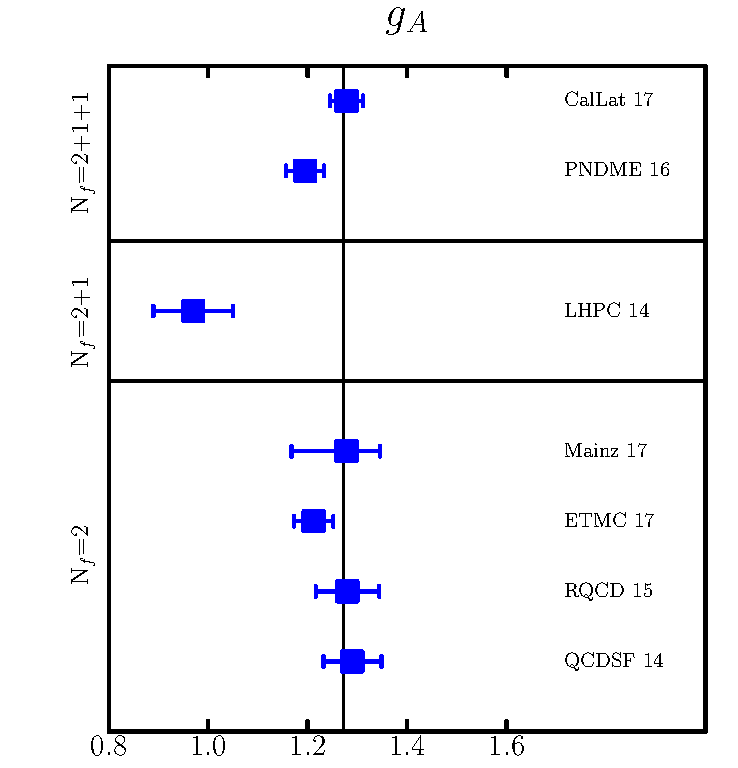
\includegraphics[scale=0.7]{plots/ga_summary.pdf}\\
\caption{\small Summary of the current status of lattice-QCD calculations of 
the axial charge, $g_A\equiv \langle 1\rangle_{\Delta u^+-\Delta d^+}$.
%
The vertical black line represents the current experimental world average 
$g_A^{\mathrm{exp}} = 1.2723(23)$~\cite{Olive:2016xmw}. 
%
The light gray bands for $N_f=2+1+1$ and $N_f=2$ represent the best-estimate 
results of Eq.~\eqref{eq:gAcriteria} and the dashed gray band for
$N_f=2+1+1$ is the fit band of Eq.~\eqref{eq:gAfit}. 
%
%The open symbols are results that are not included in the best-estimate values.
}    
\label{fig:gaLQCDstatus}
\end{figure}
%-------------------------------------------------------------------------------

In addition to the axial charge, we summarise the zeroth moments of the 
individual light quark total helicity distributions in 
Tab.~\ref{tab:polLQCDstatus0}. 
%
We summarise the status of lattice-QCD calculations of the
first moments of the polarised PDF combination 
$\langle x \rangle_{\Delta u^- - \Delta d^-}$ in Tab.~\ref{tab:polLQCDstatus1}. 
%
We use the same format as in Tab.~\ref{tab:unpolLQCDstatus1}.
%
All values are at $\mu^2=Q^2=4$ GeV$^2$.
%
Available results that have not been extrapolated to the physical pion mass
or quenched results are not reported here, but in 
Tabs.~\ref{tab:polLQCDstatus1B}-\ref{tab:polLQCDstatus2B} of
Appendix~\ref{sec:LQCDtables} for completeness.

In the case of $\langle 1 \rangle_{\Delta u^+}$ and $\langle 1 \rangle_{\Delta d^+}$,
there is only one result for each quantity available in the literature.
%
Therefore, despite the corresponding systematic uncertainties are not 
completely under control and possibly underestimated, we take the individual 
results as our benchmark values.
%
In the case of $\langle 1 \rangle_{\Delta s^+}$ and 
$\langle x \rangle_{\Delta u^- - \Delta d^-}$, instead, several results are available
in the literature, although without a full characterisation of
their systematic uncertainties.
%
We present our lattice-QCD benchmark value for these quantitites as
a best-estimate band extending from the mean minus the error of the 
smallest result to the mean plus the error of the largest. 
%
We include all results with two or more flavours of sea quarks listed in 
Tabs.~\ref{tab:polLQCDstatus0}-\ref{tab:polLQCDstatus1} respectively.

%-------------------------------------------------------------------------------
\begin{table}[t]
\renewcommand{\arraystretch}{1.2} 
\centering
\begin{threeparttable}
\begin{tabular}{llcllccccccl}
Mom. & Collab. & Ref. & $N_f$ & Status &
\begin{rotate}{70}{discretisation}\end{rotate} &
\begin{rotate}{70}{quark mass}\end{rotate} &
\begin{rotate}{70}{finite volume}\end{rotate} &
\begin{rotate}{70}{renormalisation}\end{rotate} &
\begin{rotate}{70}{excited states}\end{rotate}&
& Value \\
\midrule
$\langle 1\rangle_{\Delta u^+}$
& ETMC\,17 
  & \cite{Alexandrou:2017oeh} 
  & 2 
  & PreP 
  & \rsquare 
  & \bstar 
  & \rsquare 
  & \bstar 
  & \bstar 
  & $^*$ 
  & $0.830(26)(4)$\\
\midrule
$\langle 1\rangle_{\Delta d^+}$
& ETMC\,17  
  & \cite{Alexandrou:2017oeh} 
  & 2 
  & PreP 
  & \rsquare 
  & \bstar 
  & \rsquare  
  & \bstar 
  & \bstar 
  & $^*$ 
  & $-0.386(16)(6)$\\
\midrule
$\langle 1\rangle_{\Delta s^+}$
& $\chi$QCD\,17 
  & \cite{Gong:2015iir} 
  & 2+1 
  & P 
  & \rsquare  
  & \bcirc 
  & \bcirc  
  & \bstar 
  & \bstar
  & $^{\dagger,\triangleleft}$ 
  & -0.0403(44)(78)\\
& Engelhardt\,12 
  & \cite{Engelhardt:2012gd} 
  & 2+1 
  & P 
  & \rsquare  
  & \rsquare 
  & \bcirc  
  & \bstar  
  & \bstar  
  & $^\triangleleft$ 
  & -0.031(17)\\
& ETMC\,17 
  & \cite{Alexandrou:2017oeh} 
  & 2 
  & PreP 
  & \rsquare  
  & \bstar 
  & \rsquare  
  & \bstar  
  & \bstar 
  & $^*$ 
  & -0.042(10)(2)\\
\bottomrule
\end{tabular}
\begin{tablenotes}
\footnotesize
\item[$*$] Study employing a single physical pion mass ensemble.
\item[$\dagger$] Partially quenched simulation with $m_\pi=330$~MeV. 
Criteria applied to the valence quarks. 
\item[$\triangleleft$] Some parts of the renormalisation are estimated, 
see references for details.
\end{tablenotes}
\end{threeparttable}
\caption{\small Summary of the current status of lattice-QCD calculations 
of the zeroth moments of longitudinally polarised PDFs.}
\label{tab:polLQCDstatus0}
\end{table}
%-------------------------------------------------------------------------------

%-------------------------------------------------------------------------------
\begin{table}[t] 
\renewcommand{\arraystretch}{1.2}
\centering
\begin{threeparttable}
\begin{tabular}{llcllccccccl}
Mom. & Collab. & Ref. & $N_f$ & Status &
\begin{rotate}{70}{discretisation}\end{rotate}  &
\begin{rotate}{70}{quark mass}\end{rotate}      &
\begin{rotate}{70}{finite volume}\end{rotate}   &
\begin{rotate}{70}{renormalisation}\end{rotate} &
\begin{rotate}{70}{excited states}\end{rotate}  &
& Value \\
\toprule
$\langle x\rangle_{\Delta u^--\Delta d^-}$
& RBC 
  & \cite{Aoki:2010xg} 
  & 2+1 
  & P 
  & \rsquare  
  & \rsquare 
  & \bstar  
  & \bstar  
  & \rsquare 
  &  
  & 0.256(23)\\
& UKQCD\,10 
  & \cite{Aoki:2010xg} 
  & 2+1 
  & P 
  & \rsquare  
  & \rsquare 
  & \bstar  
  & \bstar  
  & \rsquare 
  &  
  & 0.205(59)\\
& LHPC\,10 
  & \cite{Bratt:2010jn} 
  & 2+1 
  & P 
  & \rsquare  
  & \rsquare 
  & \bcirc  
  & \bcirc  
  & \rsquare 
  &  
  & 0.1972(55)\\
& ETMC\,15 
  & \cite{Abdel-Rehim:2015owa} 
  & 2 
  & P 
  & \rsquare  
  & \bstar 
  & \rsquare  
  & \bstar  
  & \bstar 
  & $^*$ 
  & 0.229(33)\\
\bottomrule
\end{tabular}
\begin{tablenotes}
\footnotesize
\item[$*$] Study employing a single physical pion mass ensemble.
\end{tablenotes}
\end{threeparttable}
\caption{\small Summary of the current status of lattice-QCD calculations of 
moments of longitudinally polarised PDFs.}
\label{tab:polLQCDstatus1}
\end{table}
%-------------------------------------------------------------------------------

\subsubsection{Appraising global-PDF fit results}
\label{subsubsec:GPDFfits}

The current state-of-the-art for global PDF fit determinations and their 
uncertainties has been carefully assessed in dedicated reviews
recently~\cite{Forte:2013wc,Jimenez-Delgado:2013sma}. 
%
It is now recognised that the PDF uncertainty receives various contributions 
of comparable importance: the measurement uncertainty propagated from the
experimental data, uncertainties associated with incompatibility of the 
fitted experiments, procedural uncertainties such as those related to the
functional form of PDFs, and the handling of systematic errors.
%



%Here say something about how uncertainties are asseses in PDF fits.
%Say that, in comparison to lattice, the field is much more developed.

\paragraph{Unpolarised parton distributions}

We summarise the current status of global-PDF fits results of the benchmark
moments of unpolarised PDFs listed in Sec.~\ref{subsubsec:BQ} 
in Tab.~\ref{tab:unpPDFmoms}.
%
In the first columns we indicate the computed momentum, and in the subsequent 
six columns its value as obtained from the most recent available PDF 
determinations: NNPDF3.1~\cite{Ball:2017nwa},
CT14~\cite{Dulat:2015mca}, MMHT2014~\cite{Harland-Lang:2014zoa},
ABMP16~\cite{Alekhin:2017kpj} (with $n_f=4$ flavours), 
CJ15~\cite{Accardi:2016qay} and 
HERAPDF2.0~\cite{Abramowicz:2015mha} respectively.
%
The most relevant features of these PDF sets have been presented in 
Sec.~\ref{sec:unpPDFs}.
%
All values in Tab.~\ref{tab:unpPDFmoms} have been computed 
at $\mu^2=Q^2=4$ GeV$^2$. 
%
They have been obtained from the default PDF sets at the highest available 
perturbative order, which is NNLO for all of them, except for CJ15, 
for which it is NLO.
%
Uncertainties correspond to 68\% confidence levels and denote the PDF
uncertainty only.
%
In the case of the HERAPDF2.0 set, the PDF error band is the sum in quadrature 
of the statistical, model and parametrisation uncertainties.

%-------------------------------------------------------------------------------
\begin{table}[t]
\centering
\begin{tabular}{lcccccc}
\toprule
Mom. 
& NNPDF3.1 & CT14 & MMHT2014 & ABMP2016 & CJ15 & HERAPDF2.0 \\
\midrule
$\langle x \rangle_{u^+-d^+}$ 
& 0.152(3) & 0.158(6) & 0.151(4) & 0.167(4) & 0.152(2) & 0.188(3)\\
$\langle x \rangle_{u^+}$    
& 0.348(4) & 0.348(5) & 0.348(5) & 0.353(3) & 0.348(1) & 0.372(4)\\
$\langle x \rangle_{d^+}$    
& 0.196(3) & 0.190(5) & 0.197(5) & 0.186(3) & 0.196(1) & 0.185(7)\\
$\langle x \rangle_{s^+}$    
& 0.039(3) & 0.035(9) & 0.035(9) & 0.041(2) & 0.031(1) & 0.035(11)\\
$\langle x \rangle_{g}$     
& 0.410(4) & 0.416(9) & 0.411(9) & 0.412(4) & 0.416(1) & 0.401(10)\\
\bottomrule
\end{tabular}
\caption{\small Status of current global-PDF fit determinations of the 
benchmark first moments of unpolarised PDFs listed in Sec.~\ref{subsubsec:BQ}.
All values are shown at $\mu^2=Q^2=4$ GeV$^2$.}
\label{tab:unpPDFmoms}
\end{table}
%-------------------------------------------------------------------------------

In order to provide a benchmark value for the first moments of unpolarised PDFs
listed in Tab.~\ref{tab:unpPDFmoms}, we follow the latest PDF4LHC 2015 
recommendations~\cite{Butterworth:2015oua}.
%
Even though the recommendations were primarily formulated for the usage of PDFs
in LHC-related physics, and alternative recommendations have been 
suggested~\cite{Accardi:2016ndt}, we find it useful to apply them here as well.
%
The reason is twofold.
%
First, in this benchmark exercise we aim at accuracy and precision, which are 
two of the guiding principles underlying the recommendations.
%
Second, they led to the release of specific PDF sets which can be easily 
used to provide all the needed benchmark values.

While we refer the reader to Ref.~\cite{Butterworth:2015oua} for details,
here we only mention that the PDF4LHC15 PDF sets were constructed by means of
a statistical combination (an unweighted average) of the 
NNPDF3.0~\cite{Ball:2014uwa}, CT14 and MMHT2014 PDF sets.\footnote{The 
NNPDF3.1 PDF set was not available when the recommendations were formulated.}
%
The three PDF sets were selected among all the publicly available PDF sets
based on four criteria~\cite{Butterworth:2015oua}.
%
\begin{itemize}
%
\item A global data set, from a wide variety of observables and processes, 
should be included in the analysis.
%
\item Theoretical hard cross sections should be evaluated up to NNLO in a
general-mass variable-flavour number scheme with up to $n_f^{\rm max}=5$ 
active quark flavours.
%
\item The central value of the strong coupling at the $Z$-boson mass,
$\alpha_S(M_Z^2)$ should be fixed at an agred common value, consistent with the 
PDF world-average~\cite{Olive:2016xmw}.
%
\item All known experimental and procedural sources of uncertainty should be 
properly accounted for.
%
\end{itemize}
 





\paragraph{Polarised parton distributions}




%%%%%%%%%%%%%%%%%%%%%%%%%%%%%%%%%%%%%%%%%%%%%%%%%%%%%%%%%%%%%%%%%%%%%%%%%%%%%%%%
\subsection{Benchmark values}
\label{subsec:BN}

\subsubsection{Unpolarised parton distributions}

%We denote these cases in Tab.\ref{tab:LQCDunpol} with a superscript dagger.
%We provide a systematic comparison between existing lattice-QCD computations
%and global PDF fit results for the lowest two moments of unpolarized
%and longitudinally polarized PDFs. 
%
%Current lattice calculations of higher moments are not sufficiently controlled 
%to allow for a meaningful comparison between lattice and global fit results.
%
%With the exception of the axial coupling, $g_A$, there are no lattice calculations
%for which all systematics have been fully explored and controlled. Therefore, 
%for quantities other than $g_A$, we present a best-estimate band, rather than a global average. 
%This band extends from the mean minus the error of the
%smallest result to the mean plus the error of the largest, and includes all results
%with two or more flavours of sea quarks, because current studies are not sufficiently
%precise to distinguish between results with different numbers of sea quark flavours.
%In three cases, $\langle x \rangle_{u,d,s}$, $\langle x \rangle_g$, $\langle 1 \rangle_{\Delta u,\Delta d}$, there is only one
%lattice result available. For these quantities, our best-estimate band is given by this single result, but 
%it should be noted that these results may underestimate some sources of uncertainty. We denote
%these cases in Tables \ref{tab:LQCDunpol} and \ref{tab:LQCDpol0} with a superscript dagger.
%In all benchmark tables, the moments are understood to be evaluated at a scale $\mu^2 = Q^2=4$ GeV$^2$. 
%
%We provide complete listings of available results in Appendix \ref{sec:LQCDtables}.


%-------------------------------------------------------------------------------
\begin{table}[t]
\centering
\begin{tabular}{lcc}
\toprule
Moment & Lattice QCD & Global Fit\\
\midrule
$\langle x \rangle_{u^+ -d^+}$ 
& \numrange{0.119}{0.226} 
& 0.155(5)\\
$\langle x \rangle_{u^+}$     
& 0.453(75)$^\dagger$ 
& 0.347(5)\\
$\langle x \rangle_{d^+}$     
& 0.259(74)$^\dagger$ 
& 0.193(6)\\
$\langle x \rangle_{s^+}$     
& 0.092(41)$^\dagger$ 
& 0.036(6)\\
$\langle x\rangle_{g}$       
& 0.267(35)$^\dagger$ 
& 0.414(9)\\
\bottomrule
\end{tabular}
\caption{\small Benchmark values for lattice-QCD calculations and global-PDF 
fit determinations of the benchmark moments of unpolarised PDFs.
%
All values are shown at $Q^2=4$ GeV$^2$.
%
Results with a superscript~$\dagger$ are from a single lattice 
calculation; these values may underestimate some sources of uncertainty.}
\label{tab:LQCDunpol}
\end{table}
%-------------------------------------------------------------------------------

\subsubsection{Polarised parton distributions}

%-------------------------------------------------------------------------------
\begin{table}[t]
\centering
\begin{tabular}{lcc}
\toprule
Moment & Lattice QCD & Global Fit\\
\midrule
$g_A\equiv\langle 1\rangle_{\Delta u^+ - \Delta d^+}$ 
&  
& \\
$\langle 1 \rangle_{\Delta u^+}$     
& 0.830(26)$^\dagger$ 
& \\
$\langle 1 \rangle_{\Delta d^+}$     
& -0.386(17)$^\dagger$ 
& \\
$\langle 1 \rangle_{\Delta s^+}$     
& -0.052- -0.014
& \\
$\langle x\rangle_{\Delta u^- - \Delta d^-}$       
& 0.146-0.279 
& \\
\bottomrule
\end{tabular}
\caption{\small Benchmark values for lattice-QCD calculations and global-PDF 
fit determinations of the benchmark moments of polarised PDFs.
%
All values are shown at $Q^2=4$ GeV$^2$.
%
Results with a superscript~$\dagger$ are from a single lattice 
calculation; these values may underestimate some sources of uncertainty.}
\label{tab:LQCDunpol}
\end{table}
%-------------------------------------------------------------------------------













%%%%%%%%%%%%%%%%%%%%%%%%%%%%%%%%%%%%%%%%%%%%%%%%%%%%%%%%%%%%%%%%%%%%%%%%%%%%%%%%
\section{Improving PDF fits with lattice QCD calculations}
\label{sec:projections}
%%%%%%%%%%%%%%%%%%%%%%%%%%%%%%%%%%%%%%%%%%%%%%%%%%%%%%%%%%%%%%%%%%%%%%%%%%%%%%%%

In this section we aim to provide an initial estimate of the potential  impact of
present and future lattice-QCD calculations
in global unpolarised and polarised PDF fits.
%
This study will be carried out by means of the publicly available
Bayesian reweighting
method~\cite{Ball:2011gg,Ball:2010gb} applied to the
NNPDF3.1 NNLO an NNPDFpol1.1 sets.
%
We emphasize however that the qualitative results that are found here
should apply as well to other PDF sets, for example
if the Hessian profiling method~\cite{Camarda:2015zba} was used to assess the
impact of the same lattice calculations into a Hessian sets.
%
Both approximate methods allow to quantify the impact of new measurements
(or of future measurements, if pseudo-data is used) on a PDF set without
having to redo the global analysis again.

For simplicity, we will restrict  ourselves here to study the
impact of a subset of the moments that can be
evaluated using lattice QCD.
%
In particular,
we will focus on those that can be currently calculated
with the smallest uncertainties, as discussed in
Sect.~\ref{sec:benchmarking}.
%
We do not consider other of the moments discussed in
Sect.~\ref{Sec:IntroLQCD} and Appendix~\ref{sec:LQCDtables}
since these are typically affected by larger systematic uncertainties.
%
Likewise, we won't consider  in this exercise pseudo-data based on $x$-space
lattice QCD calculations, such as those from the quasi-PDF approach,
since as shown in Sect.~\ref{sec:xdependence}, despite the rapid
recent progress, existing calculations are still far to the
phenomenological PDFs.
%
We leave for future work quantifying the impact of  $x$-space
lattice QCD calculations of PDFs in the global analysis.

Taking into account
these considerations, we will consider in this analysis the following
moments.
%
For the unpolarized case, we will use
\be
  \la x\ra_{u^+}\, , \quad
\la x\ra_{d^+}\, , \quad
\la x\ra_{s^+}\, , \quad
\la x\ra_{g}\, , \quad {\rm and} \quad
\la x\ra_{u^+-d^+} \, ,
\ee
while for the polarized side, we will include instead
the following five moments:
\be
\la 1\ra_{\Delta u^+}\, , \quad
\la 1\ra_{\Delta d^+}\, , \quad
\la 1\ra_{\Delta s^+}\, , \quad
\la x\ra_{\Delta u^--\Delta d^-}\, , \quad {\rm and} \quad
\la 1\ra_{\Delta u^+ - \Delta d^+} \, .
\ee
Recall that Appendix~\ref{app:notation} contains the
explicit definitions and conventions used for these moments.
%
Therefore, we see that for the unpolarized case we include
the second moments (momentum fractions) of $q^+$ (with $q=u,d,s$),
of the gluon, and of the isoscalar combination $u^+-d^+$.
%
In the polarized case instead, we include the first moments (which
contribute to the proton spin content) of $\Delta q^+$ (with $q=u,d,s$)
and of the isoscalar combination $\Delta u^+-\Delta d^+$, as well as
the second moment of $\Delta u^- - \Delta d^-$.

In the present exercise we will consider three
different scenarios, which we denote
as Scenario A, B, and C respectively, for the total systematic
uncertainty than we associate to lattice
QCD calculations of PDF moments.
%
In Table~\ref{tab:scenarios} we summarize the
values assumed for this total uncertainty
    of the lattice QCD calculation, denoted by $\delta_L$, for each
    of the various unpolarized and polarized PDF moments that enter
    this analysis.
    %
    We emphasize that here, while trying to be reasonably
    realistic, we do not aim to associate a given scenario
    within a specific time-scale for the calculation.
    %
    Our results  merely provide an illustrative guidance about the potential
    constraining power of existing and future lattice QCD calculations
    of PDF  moments in the context
    of a global analysis.
    
    Specifically, as indicated
    in Table~\ref{tab:scenarios}, scenario A assumes that the uncertainties $\delta_L$
    for the lattice QCD calculations
    are on same the ball-park of the current ones, taking as
    representative values for the latter  those from the
    state-of-the-art lattice QCD calculations
    selected for the benchmarking exercise of Sect.~\ref{sec:benchmarking},
    and summarized in Tables~\ref{tab:BMunp} and~\ref{tab:BMpol}.
    %
    Then scenarios B and C represent two possible optimistic scenarios for the
    future improvement of these systematic uncertainties, where these are decreased
    by roughly a factor 2 and a factor 4 with respect current values.
    %
    Moreover, we emphasize that the generalization of these projections to other conceivable scenarios
    is straightforward and can be obtained from the authors upon request.
 
%%%%%%%%%%%%%%%%%%%%%%%%%%%%%%%%%%%%%%%
\begin{table}[t]
  \centering
  \renewcommand{\arraystretch}{1.3} 
  \begin{tabular}{c||ccccc}
    \hline
    Scenario &  \multicolumn{5}{c}{$\delta_L^{(i)}$ for unpolarized moments}   \\
&    $\la x\ra_{u^+}$  &   $\la x\ra_{d^+}$   &  $\la x\ra_{s^+}$  &
$\la x\ra_{g}$  &   $\la x\ra_{u^+-d^+}$  \\
    \hline
    Current  & $\sim 16\%$  &  $\sim 30\%$
    & $\sim 45\%$  & $\sim 13\%$  &  $\sim 60\%$ \\
    A   & 3\%  & 3\% &  5\% &  3\% &  5\% \\
 B   & 2\%  & 2\% &  4\% &  2\% &  4\%  \\
  C   & 1\%  & 1\% &  3\% &  1\% &  3\%  \\
    \hline
  \end{tabular}\vspace{0.7cm}
   \begin{tabular}{c||ccccc}
    \hline
    Scenario   &
    \multicolumn{5}{c}{$\delta_L^{(i)}$ for polarized moments} \\ 
& $\la 1\ra_{\Delta u^+}$  & $\la 1\ra_{\Delta d^+}$  & $\la 1\ra_{\Delta s^+}$
&  $\la x\ra_{\Delta u^--\Delta d^-}$  &  $\la 1\ra_{\Delta u^+ - \Delta d^+}$\\
    \hline
    Current  &
    $\sim 3\%$  & $\sim 5\%$ & $\sim 70\%$ & $\sim 65\%$ & $\sim 3\%$ \\
    \hline
    A   & 
    5\% &    10\%  &   100\% &    70\%  &    5\% \\
 B   &
 3\% &    5\%  &   50\% &    30\%  &    3\% \\
  C   & 1\% &    2\%  &   20\% &    15\%  &    1\% \\
    \hline
  \end{tabular}
   \caption{\small The three scenarios assumed here
     for the total percentage
     systematic uncertainty
    in future lattice QCD calculation $\delta_L$ for each
    of the unpolarized (upper) and polarized (lower table) PDF
    moments that are included
    in the present reweighting analysis.
    %
    In addition, the first line indicates the current systematic
    uncertainties of the state-of-the-art lattice QCD calculations
    selected for the benchmarking exercise of Sect.~\ref{sec:benchmarking},
    and summarized in Tables~\ref{tab:BMunp} and~\ref{tab:BMpol}
    for the unpolarized and polarized cases, respectively.
    %
    See text for more details.
\label{tab:scenarios}
  }
\end{table}
%%%%%%%%%%%%%%%%%%%%%%%%%%%%%%%%%%%%%%%

The procedure followed to quantify the impact of future
lattice QCD calculations
in PDF fits  (for the three scenarios of Table~\ref{tab:scenarios})
is common for unpolarized
and polarized global analyses.
%
We briefly describe this procedure here,
and refer to~\cite{Ball:2011gg,Ball:2010gb} for
additional details.
\begin{itemize}
\item First of all, we generate pseudo-data for the lattice QCD calculation
  of the PDF moments used in this exercise, namely $\la x\ra_{u^+}$,
$\la x\ra_{d^+}$,
$\la x\ra_{s^+}$,
$\la x\ra_{g}$, and
  $\la x\ra_{u^+-d^+}$ for the unpolarized case, and
  $\la 1\ra_{\Delta u^+}$,
$\la 1\ra_{\Delta d^+}$,
$\la 1\ra_{\Delta s^+}$,
$\la x\ra_{\Delta u^--\Delta d^-}$, and
  $\la 1\ra_{\Delta u^+ - \Delta d^+}$ for the polarized case.
  %
  We denote generically these moments by $\mathcal{F}_i$.
\item This pseudo-data, denoted by $\mathcal{F}_i^{\rm (exp)}$,
  is constructed by taking the central values from
  the corresponding NNPDF fits, NNPDF3.1 NNLO for the unpolarized case and NNPDFpol1.1 NLO
  for the polarized one.
  %
  That is, we {\it assume} for simplicity that the central value
  of such future lattice calculations would coincide with the current ones
  from the global fit.\footnote{Repeating the exercise with the actual lattice QCD
    central values would be straightforward, but
    lies beyond the scope of the present studies.}
  %
  As discussed in Sect.~\ref{sec:unpPDFs}, this corresponds to computing
  the mean over the Monte Carlo replica sample,
  \be
  \label{eq:pseudodatadef}
  \mathcal{F}_i^{\rm (exp)} \equiv \frac{1}{N_{\rm rep}}\sum_{k=1}^{N_{\rm rep}}
  \mathcal{F}_i^{\rm (k)} \, , \quad i=1,\ldots,N_{\rm mom} \, ,
  \ee
  where $N_{\rm mom}$ are the number of PDF moments that will be included
  in the reweighting, in this case $N_{\rm mom}=5$ both for the unpolarized
  and polarized cases.
  %
  To be consistent with the calculations in Sect.~\ref{sec:benchmarking},
  here the central values of the pseudo-data Eq.~(\ref{eq:pseudodatadef})
  are also evaluated at $Q^2=4$ GeV$^2$ (see Tables~\ref{tab:unpPDFmoms} and~\ref{tab:polPDFmoms}).
\item The uncertainty in the pseudo data, denoted by $\delta\mathcal{F}_i^{\rm (exp)} $,
  is taken for each moment to be the value indicated in
  Table~\ref{tab:scenarios} for each of the three scenarios.%
  That is, we have that the absolute uncertainty on the $i$-th moment
  will be given by $\delta\mathcal{F}_i^{\rm (exp)}=\delta_L^{(i)}\mathcal{F}_i^{\rm (exp)} $.
\item Using the pseudo-data (central values and total uncertainties)
  as defined above, we next need to compute
  the weights  $\omega_k$.
  %
  These weights
  quantify the agreement between each of $N_{\rm rep}$ replicas
  of the input PDF set and the corresponding lattice pseudo-data.
  %
  Specifically, first of all we compute the $\chi^2$ between each of the Monte Carlo
  replicas and the lattice pseudo-data as follows,
  \be
  \chi^{2(k)}= \sum_{i=1}^{\rm N_{\rm mom}} \frac{\lp
    \mathcal{F}_i^{\rm (k)} -\mathcal{F}_i^{\rm (exp)} \rp^2}{
    \lp \delta\mathcal{F}_i^{\rm (exp)}\rp^2} \, , \quad k=1,\ldots,N_{\rm rep} \, ,
  \ee
  assuming that there are no correlations between the different $N_{\rm mom}$ moments.
  %
  This assumption in general might not be a good approximation, since most lattice
  QCD systematic errors are correlated among the different moments, and should be
  avoided provided the full breakdown of systematic error of each quantity is available.

  
  Once the values of the $\chi^2$ have been evaluated,
  we can compute the corresponding weights for each replica.
  %
  The relation between the weights $w_k$  and the values of
  the $\chi^{2(k)}$ of each replica is the following
  \be
  \omega_k =\frac{\lp \chi^{2(k)} \rp^{(N_{\rm mom}-1)/2}\exp(-\chi^{2(k)}/2)}{
  \sum_{k=1}^{N_{\rm rep}} \lc \lp \chi^{2(k)} \rp^{(N_{\rm mom}-1)/2}\exp(-\chi^{2(k)}/2)\rc} \, ,
  \ee
  where the denominator ensures that the weight admit
  a probabilistic interpretation, that is, $\sum_k w_k=1$.
  %
  These weights represent a measure of the agreement of the individual replicas with the new pseudo-data.
  %
  For instance, replicas which have associated values
  of the moments far from the pseudo-data (within uncertainties) will
  have associated a very large weight, being thus effectively discarded.
\item These weights can be use to now recompute the PDFs, their moments,
  as well as any generic cross-section.
  %
  This procedure emulates the
  impact that adding these lattice-QCD pseudo-data in a complete PDF fit would have.
  %
  For instance, after the reweighting the mean value of
  the PDF moments should be computed as
   \be
  \label{eq:pseudodatadef1}
  \mathcal{F}_i^{\rm (rw)} \equiv \frac{1}{N_{\rm rep}}\sum_{k=1}^{N_{\rm rep}}\omega_k
  \mathcal{F}_i^{\rm (k)} \, , \quad i=1,\ldots,N_{\rm mom} \, ,
  \ee
  and same for the associated uncertainties.
\end{itemize}

One limitation of the reweighting procedure just
outlined is that it can be considered as fully 
 reliable provided only the 
  effective number of replicas $N_{\rm eff}$ that survive the reweighting
  procedure (which is a measure of the amount
  of information left) is not too small.
  %
  This effective number of replicas
    is quantified in terms of the Shannon entropy from information
    theory, namely
    \be
    \label{eq:effnrep}
    N_{\rm eff}\equiv \exp\lc \frac{1}{N_{\rm rep}}\omega_k
    \log \lp N_{\rm rep}/\omega_k\rp\rc \, .
    \ee
    Finding that $N_{\rm eff}\ll N_{\rm rep}$ means that the pseudo-data
    has a large impact on the fit, potentially leading to a large
    reduction of the PDF uncertainties.
    %
    But if the effective number of replicas becomes too
    small, say $N_{\rm eff}\lsim 25$, then the results
    become unreliable since they are affected by large
    statistical fluctuations.

    Therefore, before considering the effects
    of the lattice-QCD pseudo-data at the PDF
    level, we need to ensure that the
    three scenarios defined
    in Table~\ref{tab:scenarios} still lead
    to values of $N_{\rm eff}$ large enough for
    the reweighting procedure to be reliable.
  %
In Table~\ref{tab:neff} we indicate the effective number of replicas
    $N_{\rm eff}$, Eq.~(\ref{eq:effnrep}), remaining when the pseudo-data
    on the PDF moments is included in the global
    fit according to the 
    %
    For completeness, we also indicate here the original number
    of replicas $N_{\rm rep}$ for the original
    PDF sets, NNPDF3.1 NNLO and NNPDFpol1.1 respectively.
    %
    As we can see, there is a marked decrease of $N_{\rm rep}$
    for the three scenarios, indicating that adding the
    PDF moments leads to non-trivial constraints on the global
    fit.
    %
    For instance, in the most optimistic scenario,
    Scenario A, the effective number of replicas is around five (three)
    smaller than the starting number of replicas.

%%%%%%%%%%%%%%%%%%%%%%%%%%%%%%%%%%%%%%%%%%%%%%
\begin{table}[t]
  \centering
  \begin{tabular}{c|c|c}
    \hline
    &  NNPDF3.1 NNLO  &  NNPDFpol1.1 \\
    \hline
    \hline
    $N_{\rm rep}$ original   &   1000 &  100   \\
    \hline
     $N_{\rm eff}$ Scenario A    &   740  &  72   \\
     $N_{\rm eff}$ Scenario B    &   750   &   59  \\
     $N_{\rm eff}$ Scenario C   &   510  &   20  \\
    \hline
  \end{tabular}
  \caption{\small The effective number of replicas
    $N_{\rm eff}$, Eq.~(\ref{eq:effnrep}), remaining when the pseudo-data
    on the PDF moments is included in the global
    fit according to the scenarios outlined
    in Table~\ref{tab:scenarios}.
    %
    For completeness, we also indicate the original number
    of replicas $N_{\rm rep}$ for the original
    PDF sets, NNPDF3.1 NNLO and NNPDFpol1.1 respectively.
    \label{tab:neff}
  }
\end{table}
%%%%%%%%%%%%%%%%%%%%%%%%%%%%%%%%%%%%%%%%%%%%%%

\subsection{Impact on unpolarized global fits}
%
We start by discussing the results of applying the reweighting procedure
outlined above to a representative unpolarized
global fit, in this case the NNPDF3.1 NNLO analysis.

To begin with, in Table~\ref{tab:unpolmomentsrw} we summarize
the values of the unpolarized PDF moments
  used as pseudo-data, as well as the corresponding results
  after the reweighting has been performed for the
three scenarios summarized in 
in Table~\ref{tab:scenarios}.
%
As we can observe from this comparison, ....

%%%%%%%%%%%%%%%%%%%%%%%%%%%%%%%%%%%%%%%%%%%%%%%%%%%%%%%%
\begin{table}[h]
\centering
\begin{tabular}{c|c|c|c|c}
  \hline &  before RW  & RW Scen A  &  RW Scen B  & RW Scen C  \\
  \hline
  \hline
  $\la x\ra_{u^+}$     &  $0.348 \pm  0.004$   &  $ 0.349 \pm 0.002$     &     &   \\
  $\la x\ra_{d^+}$     &  $0.196\pm  0.004$   & $0.196 \pm0.002$      &     &   \\
  $\la x\ra_{s^+}$     & $0.0393 \pm 0.0036$   &  $0.0393\pm 0.0006$   &     &   \\
  $\la x\ra_{g}$      &   $0.4097\pm 0.0042$  &  $0.4097 \pm 0.0029$    &     &   \\
  $\la x\ra_{u^+-d^+}$  &  $0.1522 \pm 0.0033$  &  $0.1521 \pm 0.0019$   &     &   \\
  \hline
\end{tabular}
\caption{\small Values of the unpolarized PDF moments
  used as pseudo-data, as well as the corresponding results
  after the reweighting has been performed for the
three scenarios summarized in 
in Table~\ref{tab:scenarios}.
%
The PDF uncertainties quoted correspond in all cases to 68\%
CL intervals.
\label{tab:unpolmomentsrw}
}
\end{table}
%%%%%%%%%%%%%%%%%%%%%%%%%%%%%%%%%%%%%%%%%%%%%%%%%%%%%%%%

In Fig.~\ref{fig:impactUnpol} we show
percentage PDF uncertainty in NNPDF3.1 NNLO
  for the gluon and the $u^+$, $d^+$ and $s^+$ quark PDFs,
  compared to the results of including the five lattice
  QCD moments as pseudo-data points in the fit using the three
  different scenarios in  Table~\ref{tab:scenarios}.
  %
  We see a clear improvement in all the quark PDFs, specially
  for strangeness which is the one affected by larger
  PDF uncertainties to begin with.
  %
  In the case of the gluon PDF, its uncertainties are not
  affected by the inclusion of the lattice
  QCD results even in the most optimistic scenarios.

%------------------------------------------------------
\begin{figure}[!t]
\centering
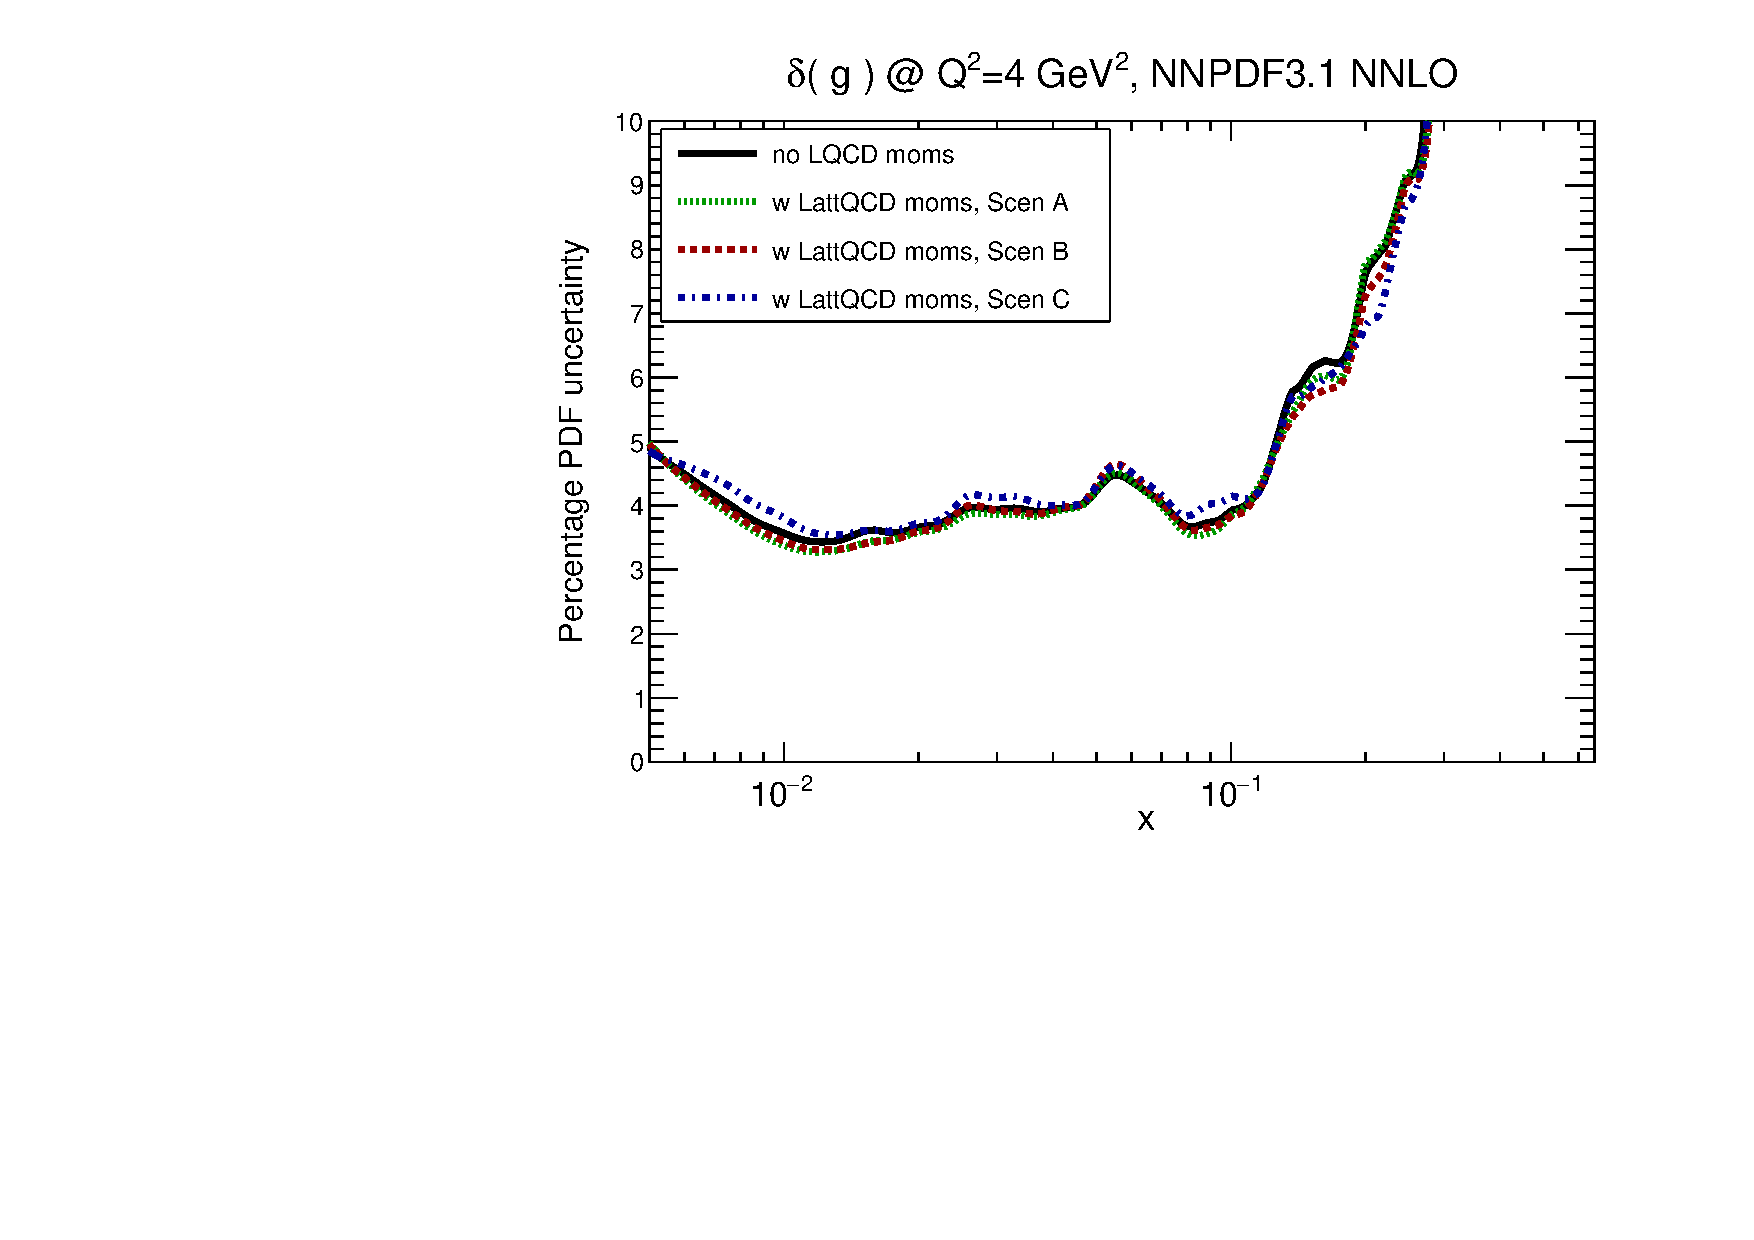
\includegraphics[scale=0.45]{plots/xg-unpol-lattice-relerr.pdf}
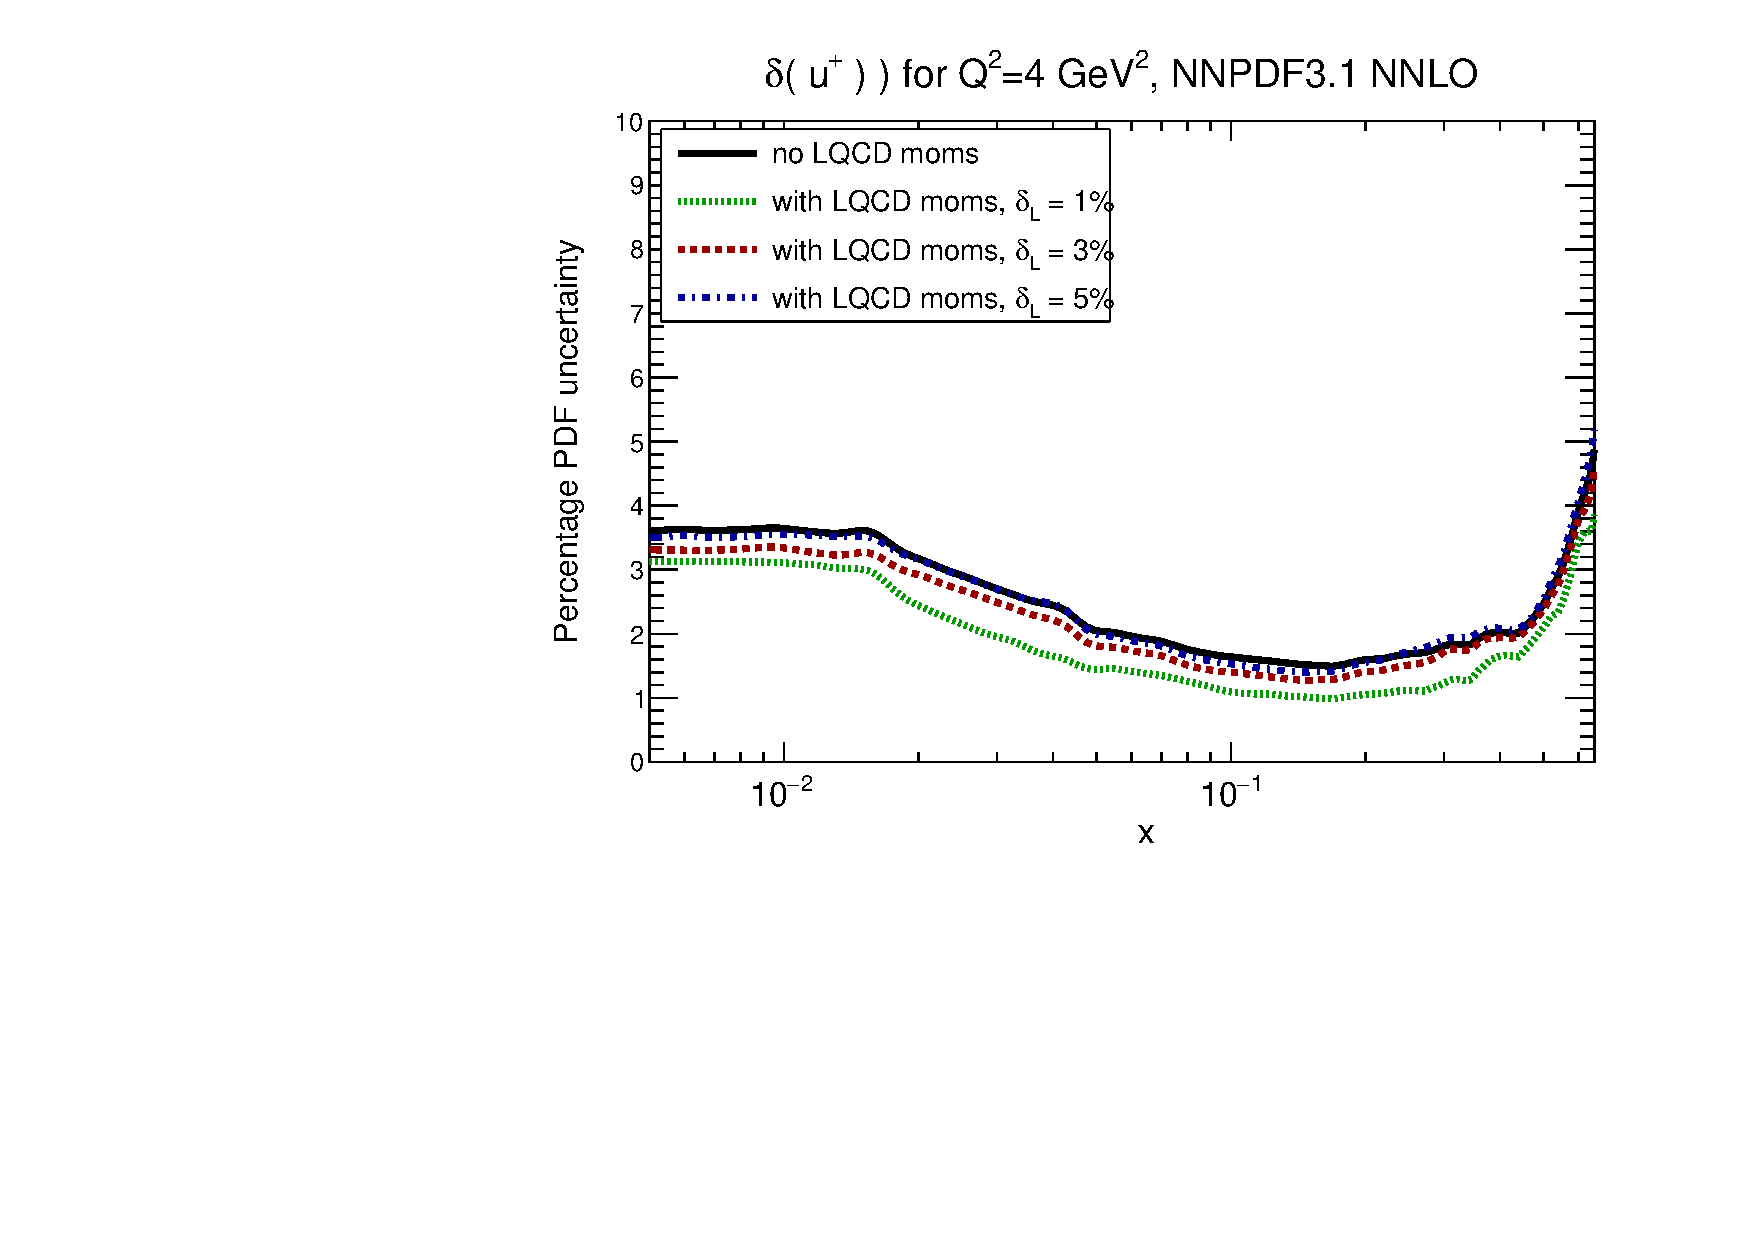
\includegraphics[scale=0.45]{plots/xup-unpol-lattice-relerr.pdf}
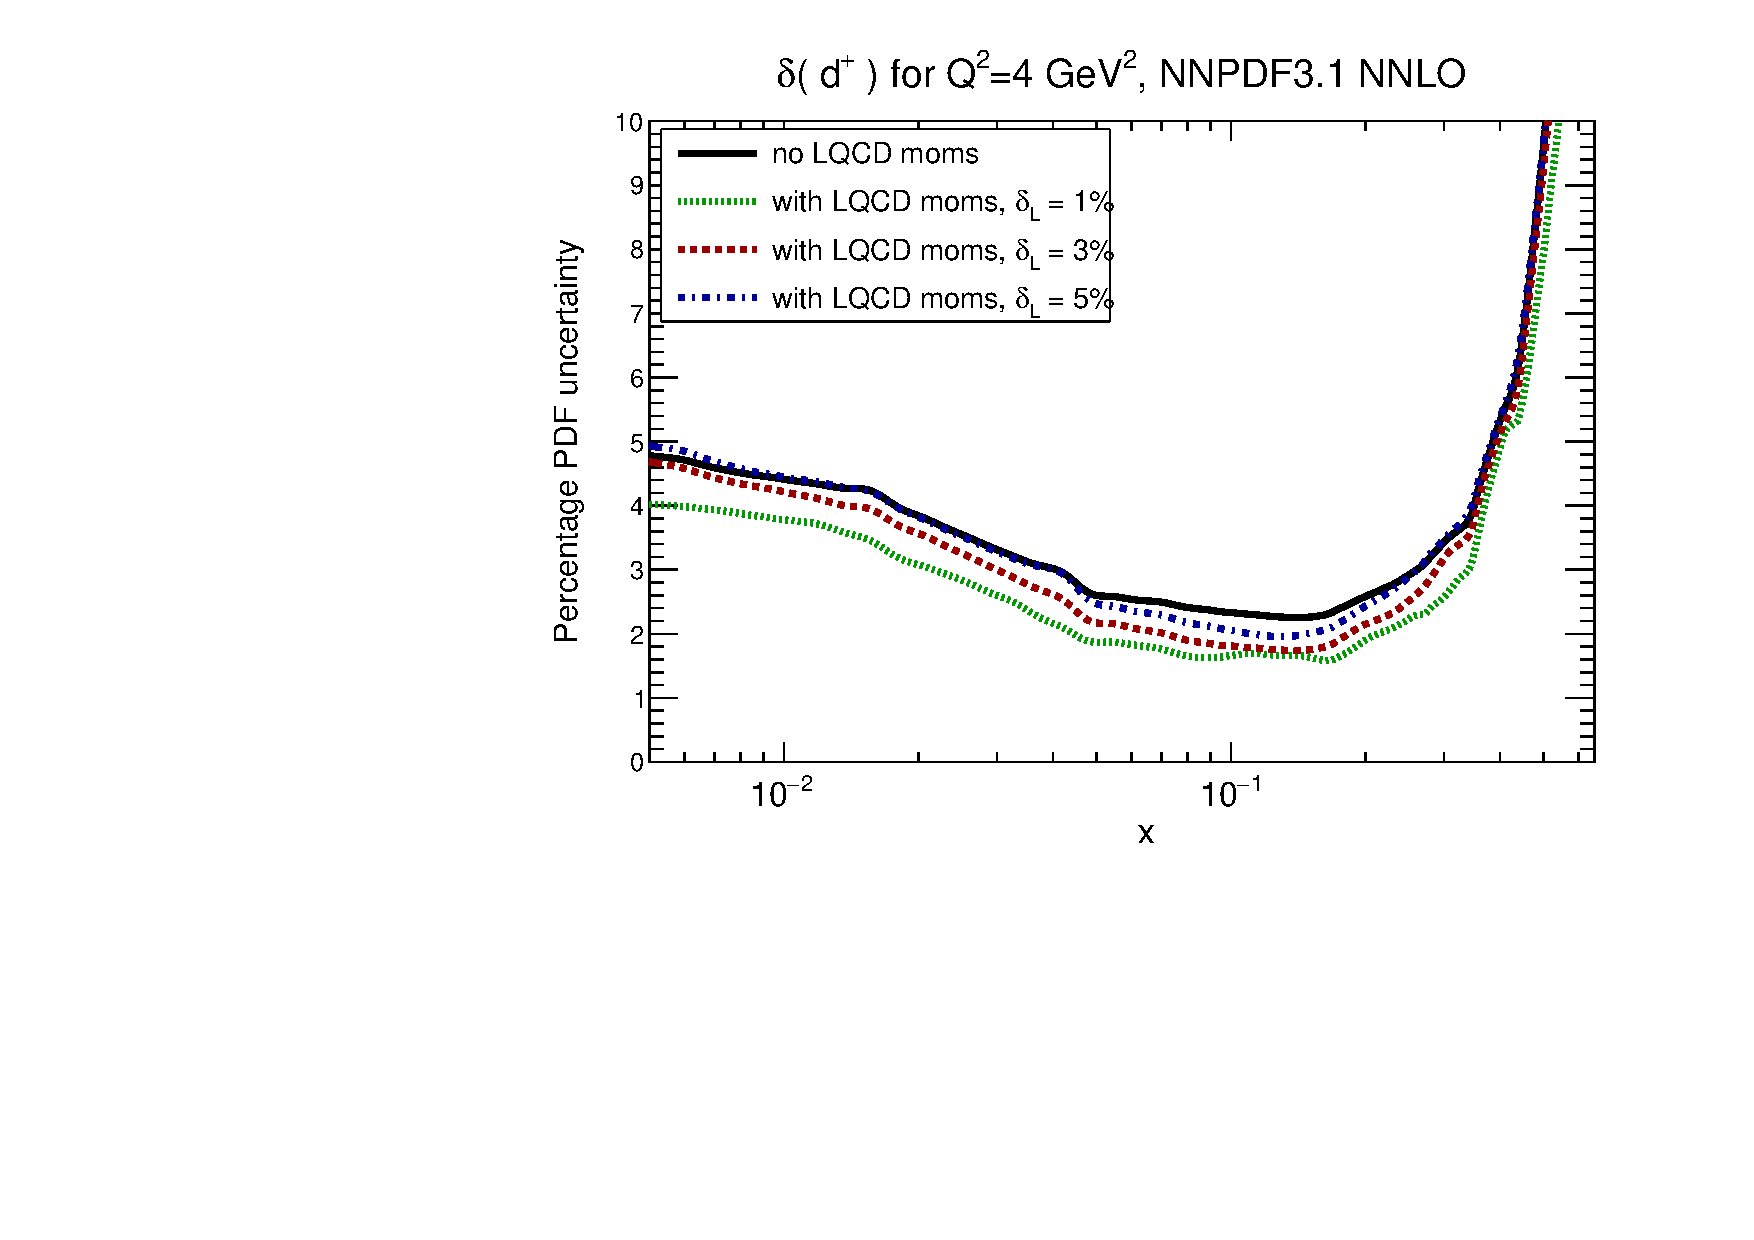
\includegraphics[scale=0.45]{plots/xdp-unpol-lattice-relerr.pdf}
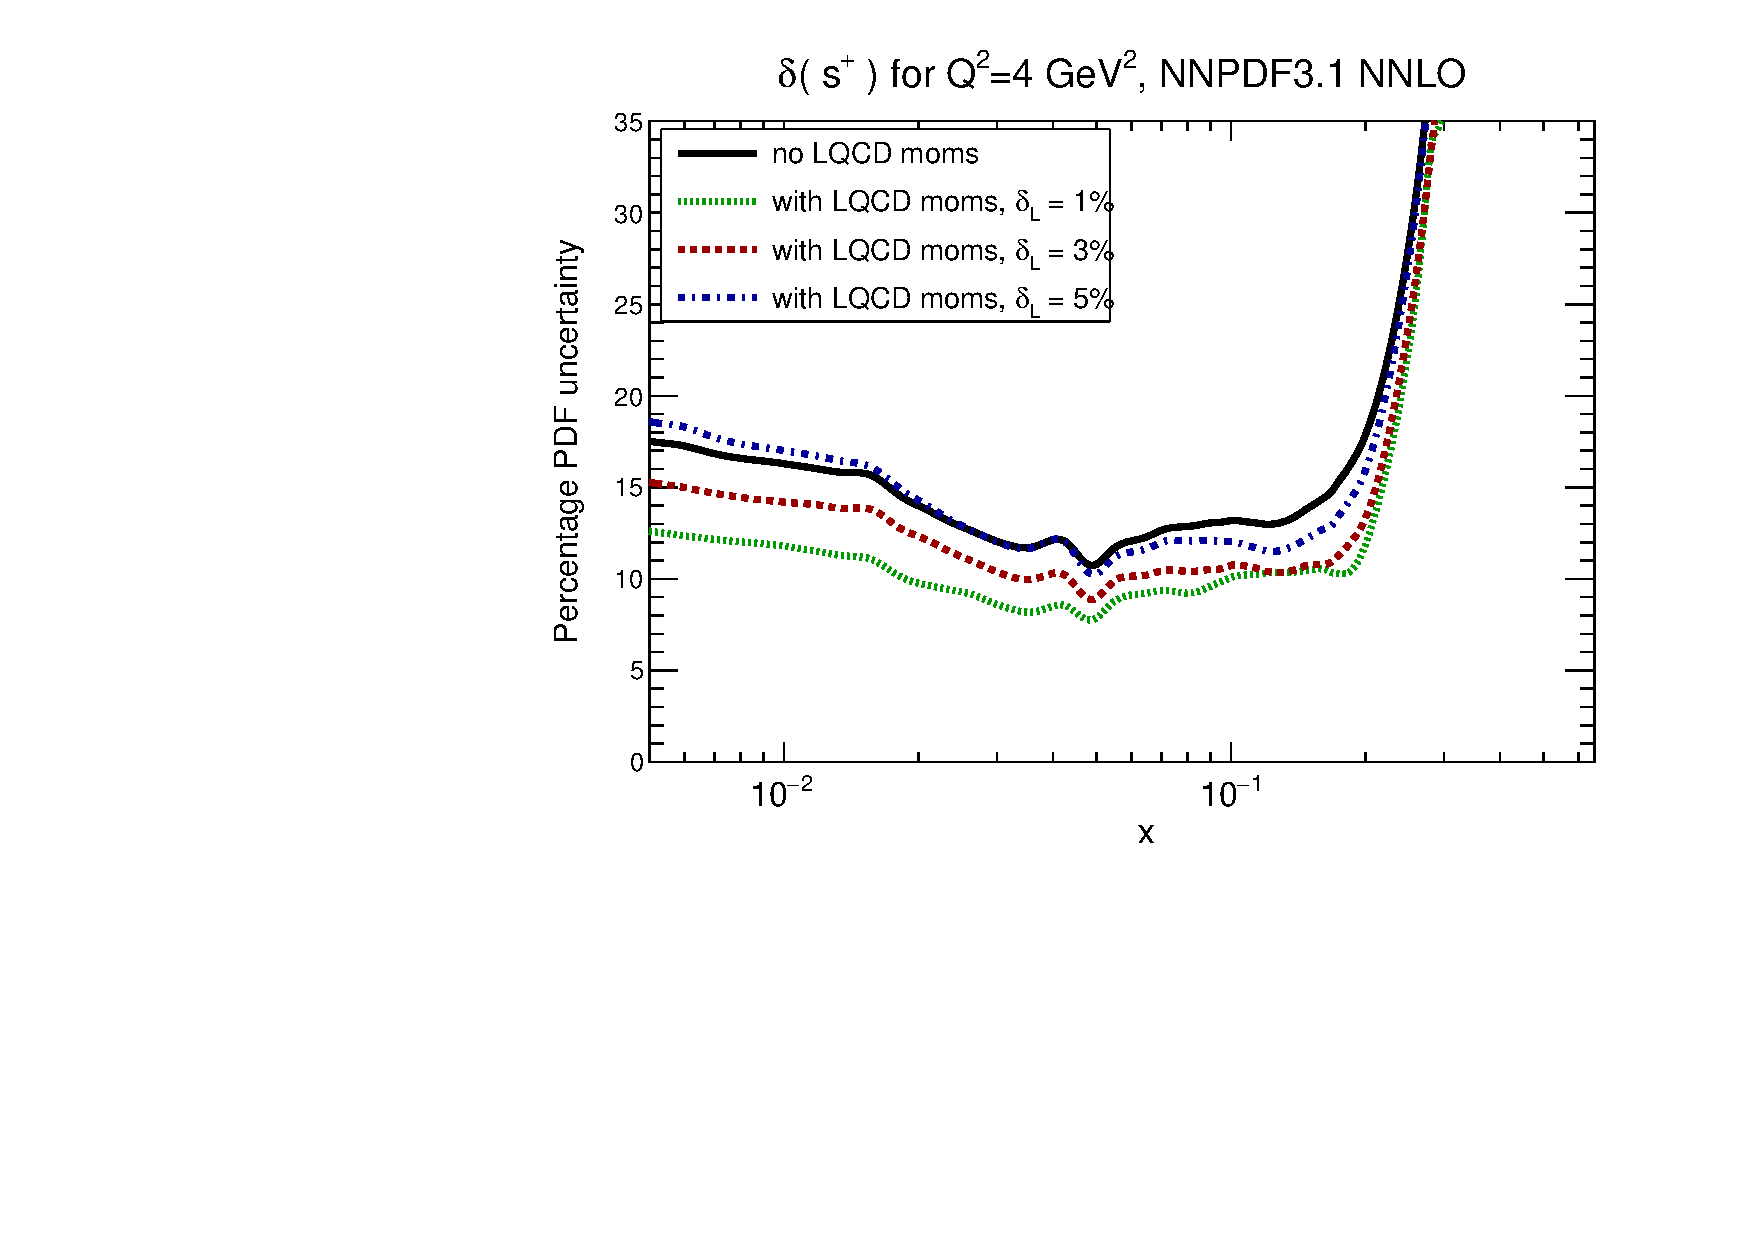
\includegraphics[scale=0.45]{plots/xsp-unpol-lattice-relerr.pdf}
\caption{\small The percentage PDF uncertainty in NNPDF3.1 NNLO
  for the gluon and the $u^+$, $d^+$ and $s^+$ quark PDFs at
  $Q^2=4$ GeV$^2$,
  compared to the results of including the five lattice
  QCD moments as pseudo-data points in the fit using the three
  different scenarios in  Table~\ref{tab:scenarios}.
  %
See text for more details.
}    
\label{fig:impactUnpol}
\end{figure}
%----------------------------------------------------------

\subsection{Impact on polarized global fits}

Next, we move to discuss the results of applying the same
reweighting procedure this time to a representative polarized
global fit, specifically NNPDFpol1.1.

First of all, in Table~\ref{tab:polmomentsrw}
we list the values of the polarized PDF moments
  used as pseudo-data, as well as the corresponding results
  after the reweighting has been performed for the
three scenarios summarized in 
in Table~\ref{tab:scenarios}.
%
The PDF uncertainties quoted correspond in all cases to 68\%
CL intervals.


%%%%%%%%%%%%%%%%%%%%%%%%%%%%%%%%%%%%%%%%%%%%%%%%%%%%%%%%
\begin{table}[h]
\centering
\begin{tabular}{c|c|c|c|c}
  \hline &  before RW  & RW Scen A  &  RW Scen B  & RW Scen C  \\
  \hline
  $\la 1\ra_{\Delta u^+}$    &  $+0.788\pm  0.079$   &  $+0.795 \pm  0.041$    &     &   \\
   $\la 1\ra_{\Delta d^+}$   &  $-0.462 \pm 0.083$  &   $-0.454\pm  0.039$  &     &   \\
  $\la 1\ra_{\Delta s^+}$    &  $-0.124\pm   0.108 $  & $ -0.115 \pm 0.021$    &     &   \\
  $\la 1\ra_{\Delta u^+ - \Delta d^+}$  & $+1.250 \pm 0.024$   & $+1.251 \pm 0.022 $    &     &   \\
  $\la x\ra_{\Delta u^--\Delta d^-}$     & $+0.196 \pm 0.014$    &  $+0.195 \pm  0.015$   &     &   \\
  \hline
\end{tabular}
\caption{\small Values of the polarized PDF moments
  used as pseudo-data, as well as the corresponding results
  after the reweighting has been performed for the
three scenarios summarized in 
in Table~\ref{tab:scenarios}.
%
The PDF uncertainties quoted correspond in all cases to 68\%
CL intervals.
\label{tab:polmomentsrw}
}
\end{table}
%%%%%%%%%%%%%%%%%%%%%%%%%%%%%%%%%%%%%%%%%%%%%%%%%%%%%%%%

In Fig.~\ref{fig:impactPol} a
similar comparison as that of Fig.~\ref{fig:impactUnpol}, now
  showing the absolute PDF uncertainties of the NNPDFpol1.1 fit
  compared to the corresponding results once the lattice pseudo-data
  on polarized moments in included in the analysis via
  reweighting.
  %
  We find that the impact of the lattice calculations
  would be more marked on the total
  strangeness PDF $\Delta s^+$.
  
%------------------------------------------------------
\begin{figure}[!t]
\centering
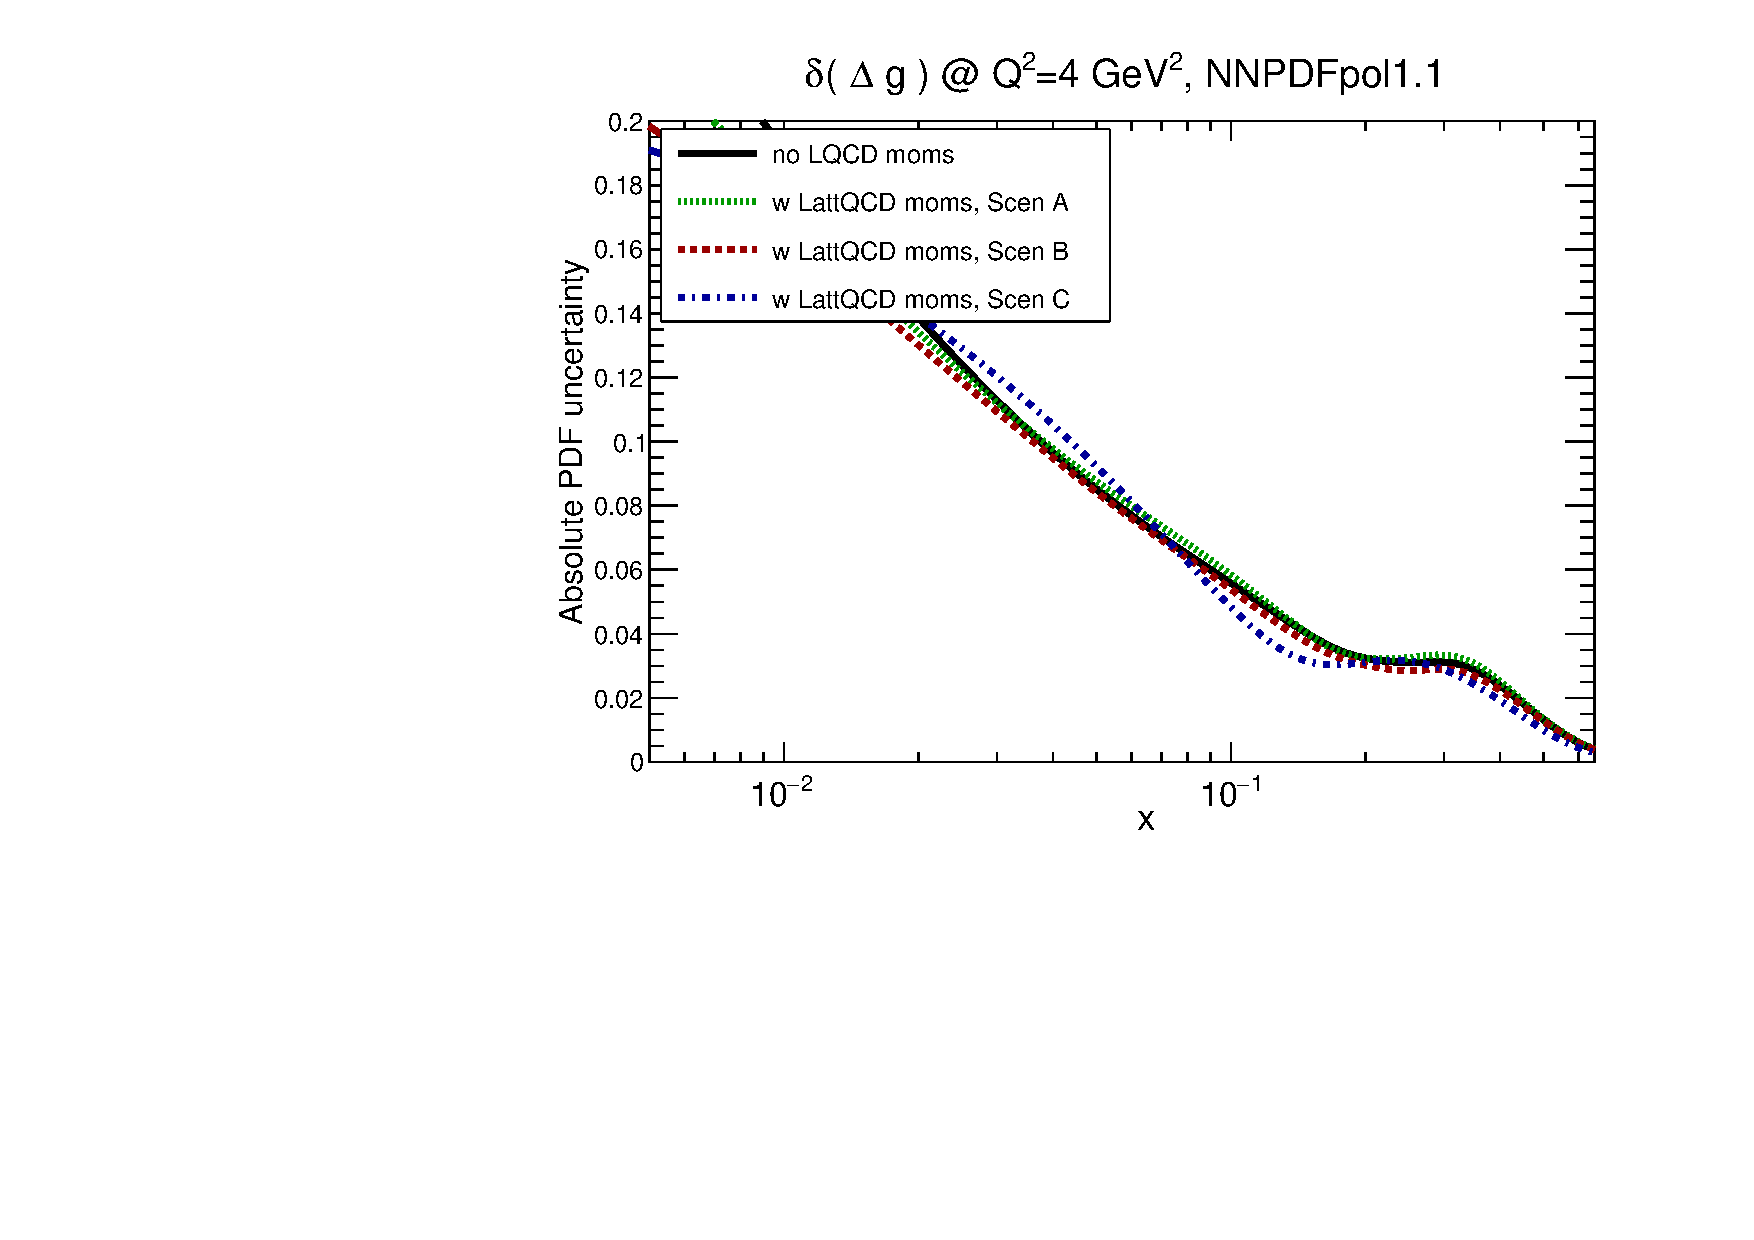
\includegraphics[scale=0.45]{plots/xg-pol-lattice-relerr.pdf}
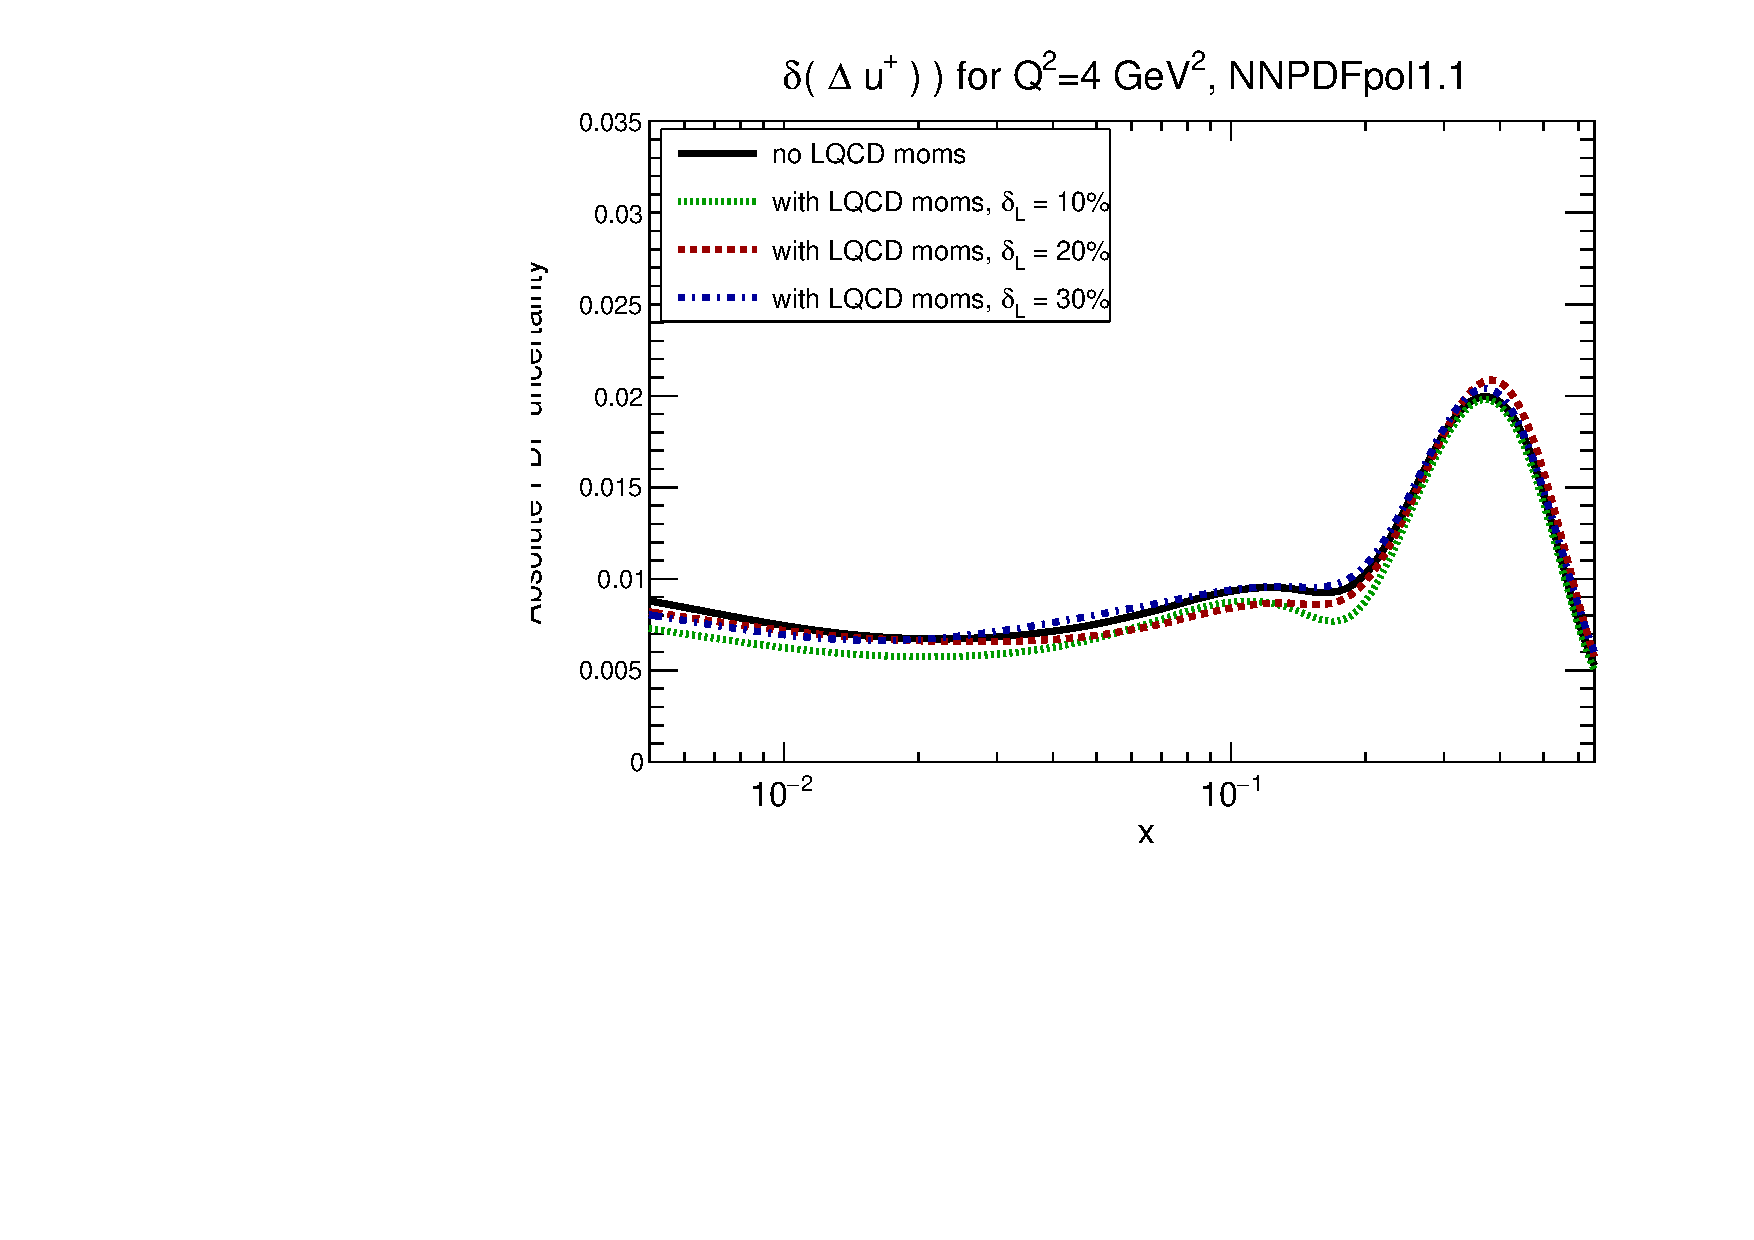
\includegraphics[scale=0.45]{plots/xup-pol-lattice-relerr.pdf}
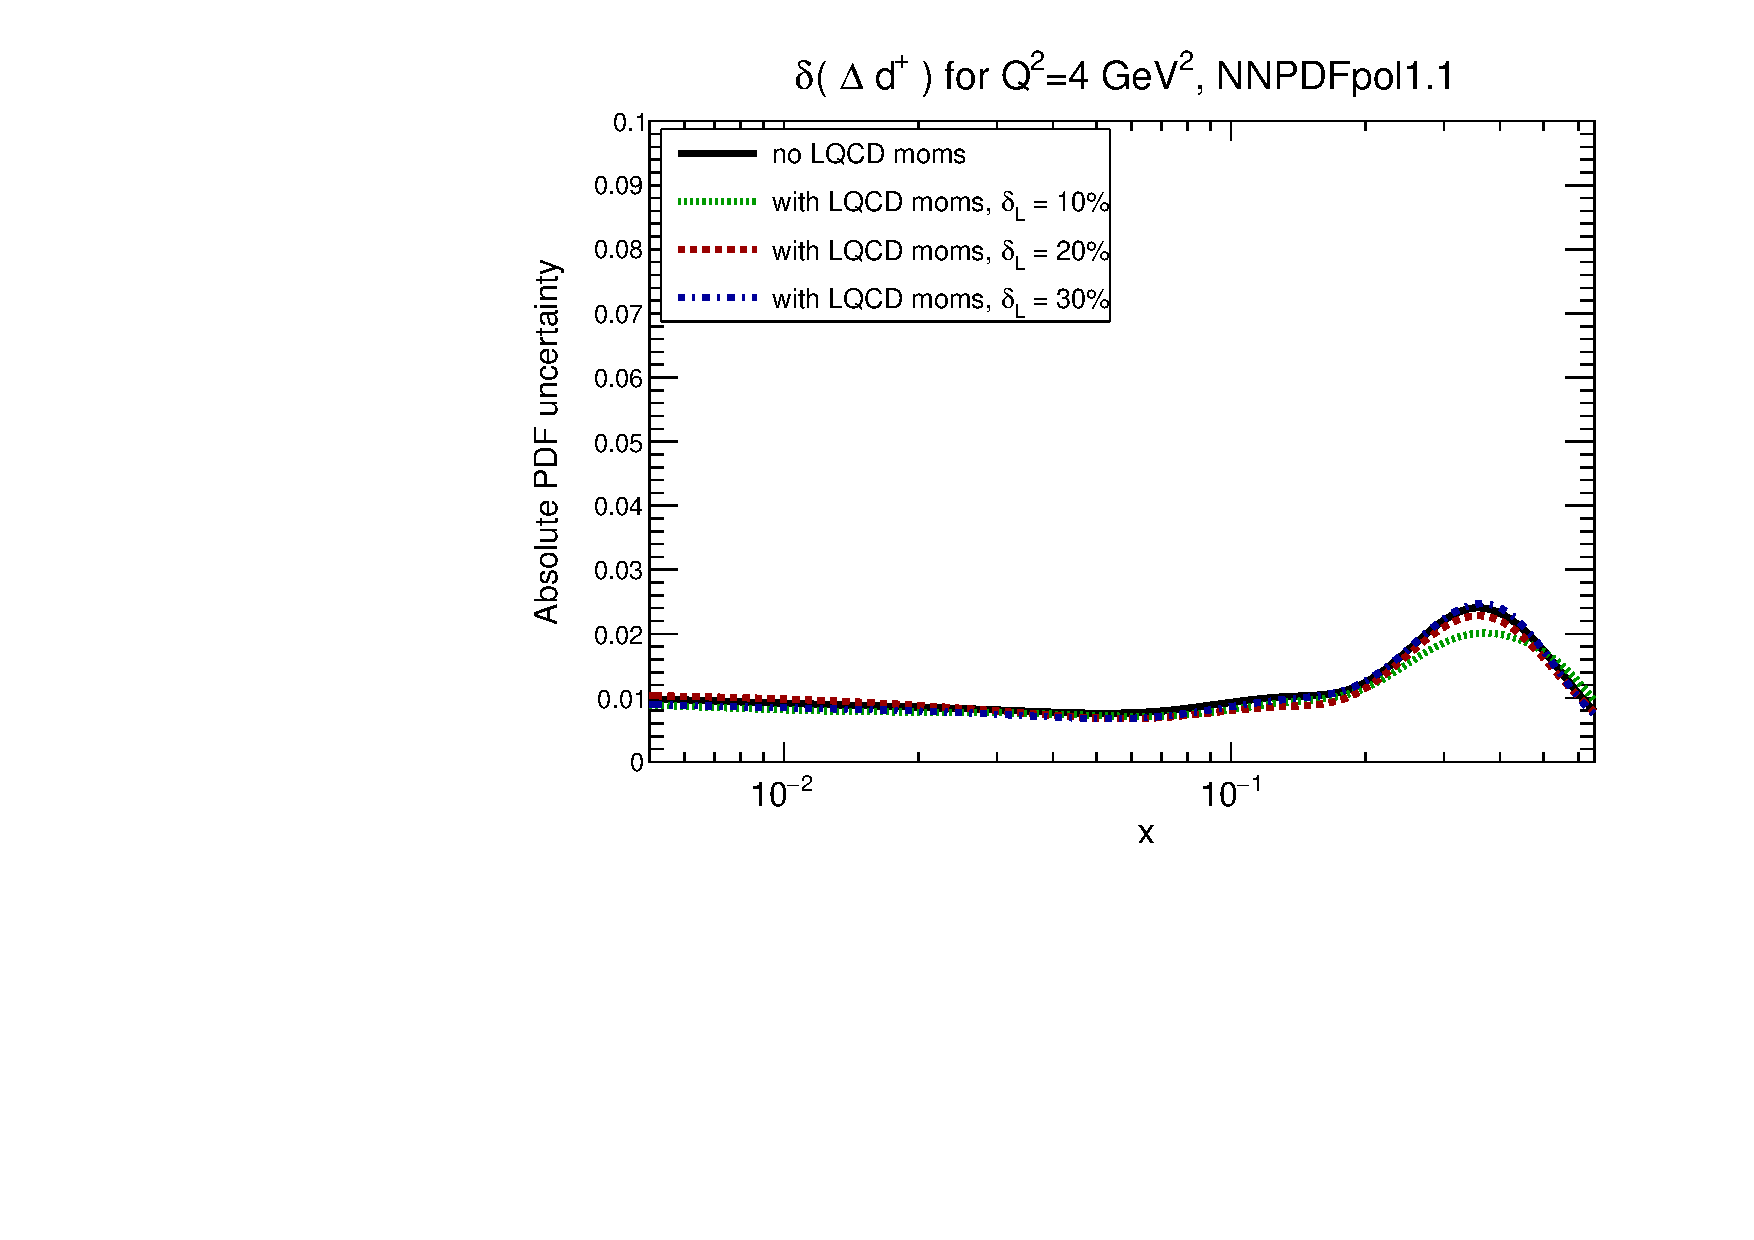
\includegraphics[scale=0.45]{plots/xdp-pol-lattice-relerr.pdf}
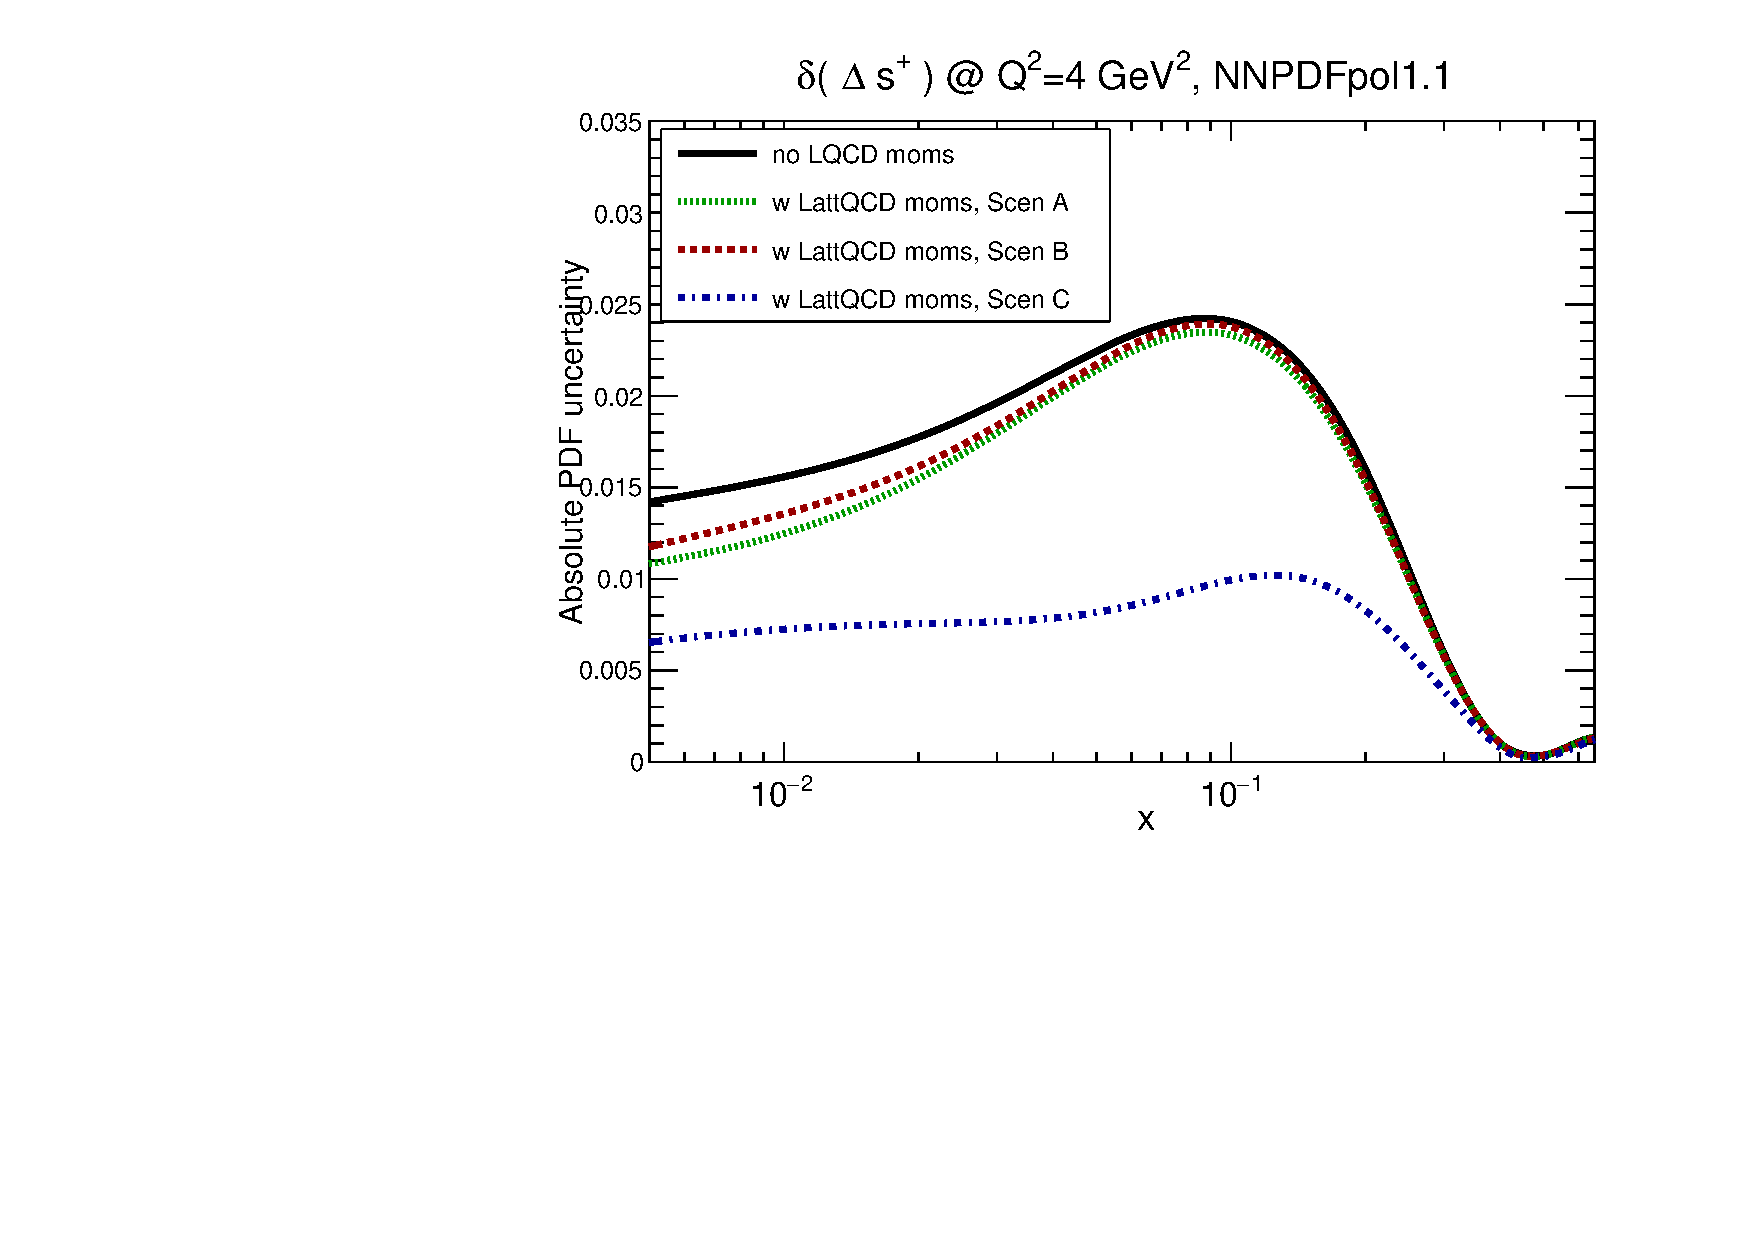
\includegraphics[scale=0.45]{plots/xsp-pol-lattice-relerr.pdf}
\caption{\small Same as Fig.~\ref{fig:impactUnpol}, now
  showing the absolute PDF uncertainties of the NNPDFpol1.1 fit
   $Q^2=4$ GeV$^2$,
  compared to the corresponding results once the lattice pseudo-data
  on polarized moments in included in the analysis via
  reweighting.
}    
\label{fig:impactPol}
\end{figure}
%----------------------------------------------------------


\clearpage


%%%%%%%%%%%%%%%%%%%%%%%%%%%%%%%%%%%%%%%%%%%%%%%%%%%%%%%%%%%%%%%%%%%%%%%%%%%%%%%%
\section{Outlook}
\label{sec:outlook}
%%%%%%%%%%%%%%%%%%%%%%%%%%%%%%%%%%%%%%%%%%%%%%%%%%%%%%%%%%%%%%%%%%%%%%%%%%%%%%%%

A brief summary of what we have learned from this report
and the outlook for future interactions between the lattice-QCD and PDF fitting communities.


%%%%%%%%%%%%%%%%%%%%%%%%%%%%%%%%%%%%%%%%%%%%%%%%%%%%%%%%%%%%%%%%%%%%%%%%%%%%%%%%
\subsection*{Acknowledgments}

We are very grateful to Jacqueline Gills for the flawless organisation
of the workshop at Balliol College and to Michelle Bosher for
invaluable help and support with the workshop logistics.
%
This workshop was partly supported by the European Research Council via
the Starting Grant {\it ``PDF4BSM - Parton Distributions in the
  Higgs Boson Era}.
%
E.~R.~N. acknowledges financial support from the
UK STFC Rutherford Grant ST/M003787/1.


\appendix

\section{Definition of the PDF moments}
\label{app:notation}

In this appendix, we summarise the convention adopted in this paper to denote the
moments of relevant unpolarised and longitudinally polarised PDF combinations.
%
Here we restrict ourselves to those
quantities which can be presently computed in lattice QCD,
although those used for benchmarks in Sect.~\ref{sec:benchmarking} are only
a subset of them.
%
In the equations below, we use the shorthand notation
\be
(\Delta)q^\pm \equiv (\Delta)q\pm(\Delta)\bar{q}\, ,\qquad q=u,d,s,c \, .
\ee
Moreover, we identify $\mu$  with the QCD factorisation scale,
and $Q$ with the characteristic scale of a given 
hard-scattering process.
%
The use of these conventions is strongly recommended for any future
comparison between lattice-QCD and global fit calculations of PDF moments.

\begin{itemize}

\item Unpolarised moments:

\begin{enumerate}

\item The first moment of the total $u^+-d^+$ PDFs
\begin{equation}
\left.\langle x\rangle_{u^+-d^+}(\mu^2)\right|_{\mu^2=Q^2}
=
\int_0^1 dx\, x\left\{u(x,Q^2)+\bar{u}(x,Q^2)-d(x,Q^2)-\bar{d}(x,Q^2)\right\} \, .
\label{eq:unpfmumdtot}
\end{equation}

\item The second moment of the valence $u^--d^-$ PDFs
\begin{equation}
\left.\langle x^2\rangle_{u^--d^-}(\mu^2)\right|_{\mu^2=Q^2}
=
\int_0^1 dx\, x^2\left\{u(x,Q^2)-\bar{u}(x,Q^2)-d(x,Q^2)+\bar{d}(x,Q^2)\right\} \, .
\label{eq:unpsmumdval}  
\end{equation}

\item The first moment of the individual quark $q^+$ total PDFs
\begin{equation}
\left.\langle x\rangle_{q^+=u^+,d^+,s^+,c^+}(\mu^2)\right|_{\mu^2=Q^2}
=
\int_0^1 dx\, x\left\{q(x,Q^2)+\bar{q}(x,Q^2)\right\} \, .
\label{eq:unpfmiqtot}
\end{equation}

\item The second moment of the individual quark $q^-$ valence PDFs
\begin{equation}
\left.\langle x^2\rangle_{q^-=u^-,d^-,s^-,c^-}(\mu^2)\right|_{\mu^2=Q^2}
=
\int_0^1 dx\, x^2\left\{q(x,Q^2)-\bar{q}(x,Q^2)\right\} \, .
\label{eq:unpsmiqval}
\end{equation}

\item The first moment of the gluon PDF
\begin{equation}
\left.\langle x \rangle_g(\mu^2)\right|_{\mu^2=Q^2}
=
\int_0^1 dx\, x\, g(x,Q^2) \, .
\label{eq:unpfmg}
\end{equation}

\end{enumerate}

\item Longitudinally polarised moments:

\begin{enumerate}

\item The zeroth moment of the total $u^+-d^+$ PDFs
\begin{equation}
\left.\langle 1 \rangle_{\Delta u^+-\Delta d^+}(\mu^2)\right|_{\mu^2=Q^2}
=
\int_0^1 dx \left\{\Delta u(x,Q^2)+\Delta\bar{u}(x,Q^2)-\Delta d(x,Q^2)-\Delta\bar{d}(x,Q^2)\right\} \, .
\label{eq:polzmumdtot}
\end{equation}

\item The first moment of the valence $u^--d^-$ PDFs
\begin{equation}
\left.\langle x\rangle_{\Delta u^--\Delta d^-}(\mu^2)\right|_{\mu^2=Q^2}
=
\int_0^1 dx\, x\left\{\Delta u(x,Q^2)-\Delta\bar{u}(x,Q^2)-\Delta d(x,Q^2)+\Delta \bar{d}(x,Q^2)\right\}
\label{eq:polfmumdval}  
\end{equation}

\item The zeroth moment of the individual quark $q^+$ total PDFs
\begin{equation}
\left.\langle 1\rangle_{q^+=\Delta u^+,\Delta d^+,\Delta s^+,\Delta c^+}(\mu^2)\right|_{\mu^2=Q^2}
=
\int_0^1 dx \left\{\Delta q(x,Q^2)+\Delta\bar{q}(x,Q^2)\right\} \, .
\label{eq:polzmiqtot}
\end{equation}

\item The first moment of the individual quark $q^-$ valence PDFs
\begin{equation}
\left.\langle x\rangle_{\Delta q^-=\Delta u^-,\Delta d^-,\Delta s^-,\Delta c^-}(\mu^2)\right|_{\mu^2=Q^2}
=
\int_0^1 dx\, x\left\{\Delta q(x,Q^2)-\Delta\bar{q}(x,Q^2)\right\} \, .
\label{eq:polfmiqval}
\end{equation}

\end{enumerate}

\end{itemize}

As discussed in Sect.~\ref{Sec:IntroPDFs}, some of these moments have a direct
physical interpretation, for instance Eq.~(\ref{eq:unpfmiqtot}) corresponds
to the proton's momentum fraction carried by a given quark flavour (and its
corresponding antiquark) at the scale $\mu$, while
Eq.~(\ref{eq:polzmiqtot}) is related to the contribution of the quark flavour
$q$ to the total proton spin.
%
Moreover, we should emphasise here that other flavour combinations as well as higher
moments are trivially computable within the global PDF fitting framework,
but we have not considered them since their evaluation within the lattice-QCD
approach is outside the reach of present capabilities.


\section{PDF moments from lattice QCD}
\label{sec:LQCDtables}

In this appendix, we summarize additional results for the moments of 
unpolarized and polarized PDFs from lattice QCD that were not discussed in 
Sect.~\ref{subsubsec:BClQCD}, either because the calculations were 
performed in the quenched approximation, or because they were not extrapolated
to the physical pion mass.

\begin{itemize}

\item In Table~\ref{tab:unpolLQCDstatus1B}, we show the first moments of 
unpolarized PDFs $\la x\ra_{u^+-d^+}$, $\la x\ra_{q^+}$ and $\la x\ra_g$
that were not included in Table~\ref{tab:unpolLQCDstatus1}.

\item In Table~\ref{tab:unpolLQCDstatus2B}, we show the second moments of 
unpolarized PDFs $\la x^2\ra_{u^--d^-}$, $\la x^2\ra_{u^-}$ and $\la x^2\ra_{d^-}$.

\item In Table~\ref{tab:polLQCDstatus1B}, we show the zeroth moments of 
polarized PDFs $\la 1\ra_{\Delta u^+}$, $\la 1\ra_{\Delta d^+}$ and 
$\la 1\ra_{\Delta s^+}$ that were not included in Table~\ref{tab:polLQCDstatus0}.

\item In Table~\ref{tab:polLQCDstatus2B}, we show the first moments of 
polarized PDFs $\la x\ra_{\Delta u^--\Delta d^-}$, $\la x\ra_{\Delta u^-}$ and  
$\la x\ra_{\Delta d^-}$ that were not included in Table~\ref{tab:polLQCDstatus1}.

\end{itemize}
%
All results are displayed at $\mu^2=4$ GeV$^2$.
%
The characterization of each source of systematic uncertainty follows the
conventions delineated in Sect.~\ref{subsubsec:BClQCD}, to which the reader 
is referred for the meaning of each symbol in 
Tables~\ref{tab:unpolLQCDstatus1B}-\ref{tab:polLQCDstatus2B}.
%
Moments are denoted according to the notation introduced in 
Appendix~\ref{app:notation}.

%-------------------------------------------------------------------------------
\begin{table}[!t]
\renewcommand{\arraystretch}{1.2} 
\centering 
\footnotesize
\begin{threeparttable}
\begin{tabular}{llcllccccccl}
\toprule
Mom. & Collab. & Ref. & $N_f$ & Status & Disc~[fm] & QM & FV & Ren & ES & & \\
\midrule
$\langle x\rangle_{u^+-d^+}$
& ETMC\,15
  & \cite{Abdel-Rehim:2015owa} 
  & 2+1+1 
  & P 
  & 0.06,0.08
  & ---  
  & \rsquare,\bstar 
  & \bstar,\bstar 
  & \rsquare,\bstar  
  &  
  & Fig.~\ref{fig:latt_res}~(a) \\
& ETMC\,15 
  & \cite{Abdel-Rehim:2015owa} 
  & 2 
  & P 
  & 0.06-0.09 
  & ---  
  & \bcirc 
  & \bstar 
  & \rsquare  
  &  
  & Fig.~\ref{fig:latt_res}~(a) \\
& RQCD\,14 
  & \cite{Bali:2014gha} 
  & 2 
  & P 
  & 0.06-0.08
  & --- 
  & \bcirc 
  & \bstar  
  & \bcirc  
  &  
  & Fig.~\ref{fig:latt_res}~(a) \\
\midrule
$\langle x\rangle_{q^+}$
& ETMC\,13 
  & \cite{Abdel-Rehim:2013wlz} 
  & 2+1+1 
  & P 
  & 0.08
  & --- 
  & \bstar  
  & \bstar  
  & \bstar  
  & $\&$ 
  & Fig.~\ref{fig:latt_res}~(b) \\
& $\chi$QCD\,13 
  & \cite{Deka:2013zha} 
  & 0 
  & P 
  & \rsquare  
  & \rsquare 
  & \rsquare  
  & \bcirc  
  & \rsquare
  & $\dagger\ddag$ 
  & $\langle x\rangle_{u^+}=0.451(37)$,\\
& $\chi$QCD\,13 
  & \cite{Deka:2013zha} 
  & 0 
  & P 
  & \rsquare  
  & \rsquare 
  & \rsquare  
  & \bcirc  
  & \rsquare
  & $\dagger\ddag$ 
  & $\langle x\rangle_{d^+}=0.188(20)$,\\
& $\chi$QCD\,13 
  & \cite{Deka:2013zha} 
  & 0 
  & P 
  & \rsquare  
  & \rsquare 
  & \rsquare  
  & \bcirc  
  & \rsquare 
  & $\dagger\ddag$ 
  & $\langle x\rangle_{s^+}=0.024(6)$\\
\midrule
$\langle x\rangle_{g}$
& ETMC\,13 
  & \cite{Alexandrou:2016ekb} 
  & 2+1+1 
  & P 
  & 0.08
  & --- 
  & \bstar  
  & \bcirc  
  & \bstar  
  &
  & Fig.~\ref{fig:latt_res}~(c) \\
& $\chi$QCD\,13 
  & \cite{Deka:2013zha} 
  & 0 
  & P 
  & \rsquare  
  & \rsquare 
  & \rsquare  
  & \bcirc   
  & \bstar 
  & $\ddag$ & 0.334(55) \\
& QCDSF\,12 
  & \cite{Horsley:2012pz} 
  & 0 
  & P 
  & \rsquare  
  & \rsquare 
  & \bstar  
  & \bstar  
  & - 
  & $\dagger$ & 0.43(7)(5) \\
\bottomrule
\end{tabular}
\begin{tablenotes}
\scriptsize
\item[$\&$] Non-singlet renormalization is applied.
\item[$\dagger$] The lightest $m_\pi$ has $Lm_\pi\ge 4.0$, however, 
$L\sim 1.6$~fm.
%\item[$\maltese$] The lightest $m_\pi$ has $Lm_\pi\ge 4.0$, however, 
%$L\sim 1.6$~fm.
\item[$\ddag$] The connected contribution is only evaluated at one $t_{sep}$.
\end{tablenotes}
\end{threeparttable}
\caption{\small Status of current lattice-QCD calculations of the first 
moments of unpolarized PDFs.
%
All results are quoted at $\mu^2=4\mbox{ GeV}^2$.
%
We use the abbreviations Disc (discretization), QM (quark mass),
FV (finite volume), Ren (renormalization) and ES (excited states)
to denote the corresponding sources of uncertainty.}
\label{tab:unpolLQCDstatus1B}
\end{table}
%-------------------------------------------------------------------------------

%-------------------------------------------------------------------------------
\begin{table}[!t]
\renewcommand{\arraystretch}{1.2} 
\centering
\footnotesize
\begin{threeparttable}
\begin{tabular}{llcllccccccl}
\toprule
Mom. & Collab. & Ref. & $N_f$ & Status & Disc & QM & FV & Ren & ES & & \\
\midrule
$\langle x^2\rangle_{u^--d^-}$
& LHPC and SESAM\,02 
  & \cite{Dolgov:2002zm} 
  & 2 
  & P 
  & \rsquare 
  & \rsquare 
  & \rsquare 
  & \bcirc 
  & \rsquare 
  &  
  & 0.145(69)\\
& QCDSF\,05 
  &\cite{Gockeler:2004wp} 
  & 0 
  & P 
  & \rsquare  
  & \rsquare 
  & \rsquare  
  & \bstar  
  & \rsquare 
  &  
  & 0.083(17)\\
& LHPC and SESAM\,02 
  &\cite{Dolgov:2002zm} 
  & 0 
  & P 
  & \rsquare 
  & \rsquare 
  & \rsquare 
  & \bcirc 
  & \rsquare 
  &  
  & 0.090(68)\\
\midrule
$\langle x^2\rangle_{u^-}$
  & $\chi$QCD\,09 
  & \cite{Deka:2008xr} 
  & 0 
  & P 
  & \rsquare  
  & \rsquare 
  & \rsquare  
  & \bcirc  
  & \rsquare 
  & $\ast$  
  & $0.117(18)$ \\
\midrule
$\langle x^2\rangle_{d^-}$
  & $\chi$QCD\,09 
  & \cite{Deka:2008xr} 
  & 0 
  & P 
  & \rsquare  
  & \rsquare 
  & \rsquare  
  & \bcirc  
  & \rsquare 
  & $\ast$  
  & $0.052(9)$\\
\bottomrule
\end{tabular}
\begin{tablenotes}
\scriptsize
\item[$\ast$] Only the connected contribution is included.
\end{tablenotes}
\end{threeparttable}
\caption{\small Same as Table~\ref{tab:unpolLQCDstatus1B}, but for 
second moments of unpolarized PDFs.}
\label{tab:unpolLQCDstatus2B} 
\end{table}
%-------------------------------------------------------------------------------

%-------------------------------------------------------------------------------
\begin{table}[!t]
\renewcommand{\arraystretch}{1.2} 
\centering
\footnotesize
\begin{threeparttable}
\begin{tabular}{llcllccccccl}
\toprule
Mom. & Collab. & Ref. & $N_f$ & Status & Disc~[fm] & QM & FV & Ren & ES & & \\
\midrule
$\langle 1\rangle_{\Delta u^+, \Delta d^+}$
& ETMC\,13 
  &\cite{Abdel-Rehim:2013wlz} 
  & 2+1+1 
  & P 
  & 0.08  
  & --- 
  & \bstar  
  & \bstar  
  & \bstar  
  & $\&$ 
  & Fig.~\ref{fig:latt_res}~(e)\\
& LHPC\,17 
  & \cite{Green:2017keo} 
  & 2+1 
  & P 
  & 0.11 
  & --- 
  & \bstar  
  & \bstar  
  & \bstar 
  &  
  & Fig.~\ref{fig:latt_res}~(e)\\
& QCDSF/CSSM\,15 
  & \cite{Chambers:2015bka}  
  & 2+1 
  & P 
  & 0.07  
  & --- 
  & \bstar 
  & \bstar  
  & \bstar   
  & %$\diamond$  
  & Fig.~\ref{fig:latt_res}~(e) \\
& QCDSF\,11 
  & \cite{QCDSF:2011aa}  
  & 2 
  & P 
  & 0.07  
  & --- 
  & \bstar 
  & \bstar  
  & \rsquare   
  & $\$$  
  & Fig.~\ref{fig:latt_res}~(e)\\
\midrule
$\langle 1\rangle_{\Delta s^+}$
  & ETMC\,13 
  & \cite{Abdel-Rehim:2013wlz} 
  & 2+1+1 
  & P 
  & 0.08  
  & --- 
  & \bstar  
  & \bstar  
  & \bstar  
  & $\&$ 
  & Fig.~\ref{fig:latt_res}~(d)\\
& LHPC\,17 
  & \cite{Green:2017keo} 
  & 2+1 
  & P 
  & 0.11 
  & --- 
  & \bstar  
  & \bstar  
  & \bstar 
  &  
  & Fig.~\ref{fig:latt_res}~(d) \\
& QCDSF/CSSM\,15 
  &\cite{Chambers:2015bka}  
  & 2+1 
  & P 
  & 0.07  
  & --- 
  & \bstar 
  & \bstar  
  & \bstar   
  & %$\diamond$  
  & Fig.~\ref{fig:latt_res}~(d) \\
& QCDSF\,11 
  & \cite{QCDSF:2011aa}  
  & 2 
  & P 
  & 0.07  
  & --- 
  & \bstar 
  & \bstar  
  & \bstar   
  & $\$$  
  & Fig.~\ref{fig:latt_res}~(d) \\
\bottomrule
\end{tabular}
\begin{tablenotes}
\scriptsize
\item[$\&$] Non-singlet renormalization is applied.
%\item[$\diamond$] Feynman-Hellmann approach is employed.
\item[$\$$] The mixing with $\langle x\rangle_{q^+}$ is small so only the 
excited state analysis for $\langle x\rangle_g$ is considered.
\end{tablenotes}
\end{threeparttable}
\caption{\small Same as Table~\ref{tab:unpolLQCDstatus1B}, but for 
zeroth moments of polarized PDFs.}
\label{tab:polLQCDstatus1B}
\end{table}
%-------------------------------------------------------------------------------

%-------------------------------------------------------------------------------
\begin{table}[!t]
\renewcommand{\arraystretch}{1.2} 
\centering
\footnotesize
\begin{threeparttable}
\begin{tabular}{llcllccccccl}
\toprule
Mom. & Collab. & Ref. & $N_f$ & Status &  
Disc~[fm] & QM & FV & Ren & ES & &  \\
\midrule
$\langle x\rangle_{\Delta u^--\Delta d^-}$
& ETMC\,15 
  & \cite{Abdel-Rehim:2015owa} 
  & 2+1+1 
  & P 
  & 0.06,0.08  
  & --- 
  & \rsquare,\bstar 
  & \bstar,\bstar 
  & \rsquare,\bstar  
  &   
  & Fig.~\ref{fig:latt_res}~(f) \\
& ETMC\,15 
  & \cite{Abdel-Rehim:2015owa} 
  & 2 
  & P 
  & 0.06-0.09  
  & --- 
  & \bcirc 
  & \bstar 
  & \rsquare 
  &  
  & Fig.~\ref{fig:latt_res}~(f) \\
\midrule
$\langle x\rangle_{\Delta u^-}$
& ETMC\,13 
  &\cite{Abdel-Rehim:2013wlz} 
  & 2+1+1 
  & P 
  & 0.08  
  & $373$~MeV 
  & \bstar  
  & \bstar  
  & \bstar 
  & $\&$ 
  &  $0.214(11)$\\
\midrule
$\langle x\rangle_{\Delta d^-}$
& ETMC\,13 
  & \cite{Abdel-Rehim:2013wlz} 
  & 2+1+1 
  & P 
  & 0.08  
  & $373$~MeV 
  & \bstar  
  & \bstar  
  & \bstar 
  & $\&$ 
  & $0.083(11)$\\
\bottomrule
\end{tabular}
\begin{tablenotes}
\scriptsize
\item[$\&$] Nonsinglet renormalization is applied.
\end{tablenotes}
\end{threeparttable}
\caption{\small Same as Table~\ref{tab:unpolLQCDstatus1B}, but for
first moments of polarized PDFs.}
\label{tab:polLQCDstatus2B}
\end{table}
%-------------------------------------------------------------------------------

We also provide tables with full bibliographic details.
%
\begin{itemize}
%
\item In Table~\ref{tab:latticebibfirst}, for the axial coupling 
$g_A\equiv\langle 1\rangle_{\Delta u^+-\Delta d^+}$.
%
We do not include quenched results, perturbatively renormalized results, 
and conference proceedings results.

\item In Table~\ref{tablenonisovectorquarkspins}, for the non-isovector quark 
spins.

\item In Table~\ref{tab:unpolarizedisotriplet}, for $\langle x\rangle_{u^+-d^+}$.
%
We omit quenched and non-renormalized results.

\item In Table~\ref{tab:nonisovectormomfrac}, for the non-isovector momentum 
fractions.

\item In Table~\ref{tab:nonisopolcase}, for 
$\langle x\rangle_{\Delta u^--\Delta d^-}$.

\item In Table~\ref{tab:latticebiblast} for  higher moments of unpolarized
  and polarized PDFs.

\end{itemize}

%-------------------------------------------------------------------------------
\begin{table}[!t]
\renewcommand{\arraystretch}{1.2} 
\centering
\footnotesize
\begin{threeparttable}
\begin{tabular}{llllll}
\toprule
Ref. & Sea quarks & Valence quarks & Renormalization & 
$N_{\Delta t}$ & $m_\pi$ (MeV)\\
\midrule
  Mainz '17b* \cite{Capitani:2017qpc} &
  2 clover & clover & Schr\"odinger functional & 4--6 & 193--473\\

  ETMC '17b \cite{Alexandrou:2017hac} &
  2 clover-TM & clover-TM & Rome-Southampton & 3 & 131\\

  CalLat '17b \cite{Berkowitz:2017gql} &
  2+1+1 staggered & domain wall & Rome-Southampton & all & 131--313 \\

  LHPC '17 \cite{Green:2017keo} &
  2+1 clover & clover & Rome-Southampton & 5 & 317 \\

  NME '17 \cite{Yoon:2016jzj} &
  2+1 clover & clover & Rome-Southampton & 1**,4--5 & 172--285 \\

  Mainz '17a \cite{vonHippel:2016wid} &
  2 clover & clover & Schr\"odinger functional & 4--6 & 193--456\\

  Dragos et al.\ '16 \cite{Dragos:2016rtx} &
  3 clover & clover & Rome-Southampton & 1,2**,5 & 460 \\

  PNDME '16 \cite{Bhattacharya:2016zcn} &
  2+1+1 staggered & clover & Rome-Southampton & 3--5 & 128--319\\

  $\chi$QCD '16 \cite{Yang:2015zja} &
  2+1 domain wall & overlap & $Z_A/Z_V=1$ & 3 & 330 \\

  ETMC '15b \cite{Abdel-Rehim:2015owa} &
    2 clover-TM & \multicolumn{4}{l}{superseded by ETMC '17} \\
  & 2 twisted mass & twisted mass & Rome-Southampton & 1 & 262--470\\
  & 2+1+1 twisted mass & twisted mass & & 1, 4 & 213, 373\\

  RQCD '15 \cite{Bali:2014nma} &
  2 clover & clover & Rome-Southampton & 1--5 & 150--490\\

  PNDME '14 \cite{Bhattacharya:2013ehc} &
  \multicolumn{5}{l}{superseded by PNDME '16} \\

  QCDSF '14 \cite{Horsley:2013ayv} &
  2 clover & clover & $g_A/f_\pi \times f_\pi^\text{phys}$ & 1,5 & 157--1591 \\

  LHPC '14 \cite{Green:2012ud} &
  2+1 clover & clover & Rome-Southampton & 3 & 149--356\\

  ETMC '13 \cite{Alexandrou:2013joa} &
  \multicolumn{5}{l}{superseded by ETMC '15b} \\

  CSSM '13 \cite{Owen:2012ts} &
  2+1 clover & clover & Schr\"odinger functional & 1**$^\dagger$ & 290 \\

  Mainz '12 \cite{Capitani:2012gj} &
  \multicolumn{5}{l}{superseded by Mainz '17b} \\

  ETMC '11 \cite{Alexandrou:2011nr} &
  \multicolumn{5}{l}{superseded by ETMC '15b} \\

  LHPC '10 \cite{Bratt:2010jn} &
  2+1 staggered & domain wall & $A_\mu/\mathcal{A}_\mu$ ratio & 1--2 & 293--758 \\

  RBC+UKQCD '09 \cite{Yamazaki:2009zq} &
  2+1 domain wall & domain wall & $Z_A/Z_V=1$ & 1 & 329--668 \\

  RBC+UKQCD '08 \cite{Yamazaki:2008py} &
  \multicolumn{5}{l}{superseded by RBC+UKQCD '09} \\

  RBC '08 \cite{Lin:2008uz} &
  2 domain wall & domain wall & $Z_A/Z_V=1$ & 1--2 & 493--695 \\

  LHPC '08 \cite{Hagler:2007xi} &
  \multicolumn{5}{l}{superseded by LHPC '10} \\

  Alexandrou et al.\ '07 \cite{Alexandrou:2007xj} &
  2 Wilson & Wilson & Rome-Southampton & 1 & 384--691 \\

  LHPC '06 \cite{Edwards:2005ym} &
  \multicolumn{5}{l}{superseded by LHPC '10} \\

  QCDSF '06 \cite{Khan:2006de} &
  \multicolumn{5}{l}{superseded by QCDSF '14} \\
\bottomrule
\end{tabular}
\begin{tablenotes}
\scriptsize
\item[$*$] Preprint.
\item[$**$] A variationally optimized interpolating operator is employed.
\item[$\dagger$] Carried out with a single fixed source-operator separation 
and all source-sink separations.
\end{tablenotes}
\end{threeparttable}
\caption{\small Full details of lattice-QCD calculations of the axial 
coupling $g_A\equiv\langle 1\rangle_{\Delta u^+-\Delta d^+}$.
%
We omit quenched results, perturbatively renormalized results, and conference 
proceedings.}
\label{tab:latticebibfirst}
\end{table}
%-------------------------------------------------------------------------------

%-------------------------------------------------------------------------------
\begin{table}[!t]
\renewcommand{\arraystretch}{1.2} 
\centering
\footnotesize
\begin{threeparttable}
\begin{tabular}{lllll}
\toprule
Ref. & Flavors & Sea quarks & Valence quarks & Renormalization \\
\midrule

  ETMC '17b \cite{Alexandrou:2017hac} &
  $u,d,s,c$ & 2 clover-TM & clover-TM & Rome-Southampton \\

  ETMC '17c \cite{Alexandrou:2017oeh} &
  $u,d,s$ & 2 clover-TM & clover-TM & Rome-Southampton \\

  $\chi$QCD '17b \cite{Gong:2015iir} &
  $s,c$ & 2+1 domain wall & overlap & single-flavor anomalous WI \\

  LHPC '17 \cite{Green:2017keo} &
  $u,d,s$ & 2+1 clover & clover & Rome-Southampton \\

  CSSM and &
  $u+d+s$ &
  2+1, 3 clover & clover & Rome-Southampton \\
  QCDSF/UKQCD '15 \cite{Chambers:2015bka} & conn.\ / disc. & & & \\

  ETMC '14 \cite{Abdel-Rehim:2013wlz} &
  $u+d,s$ & 2+1+1 twisted mass & twisted mass & non-singlet Rome-Southampton\\

  Engelhardt '12 \cite{Engelhardt:2012gd} &
  $s$ & 2+1 staggered & domain wall & non-singlet $A_\mu/\mathcal{A}_\mu$ ratio \\

  QCDSF '12 \cite{QCDSF:2011aa} &
  $u,d,s$ & 2 clover & clover & non-singlet Rome-Southampton \\
  & & & &+ two-loop singlet-nonsinglet\\

  Babich et al.\ '10 \cite{Babich:2010at} &
  $s$ & 2 aniso-clover & aniso-clover & none \\

  SESAM '99 \cite{Gusken:1999as} &
  $u,d,s$ & 2 Wilson & Wilson & one loop \\

  $\chi$QCD '95 \cite{Dong:1995rx} &
  $u,d,s$ & quenched & Wilson & one loop \\

  Fukugita et al.\ '95 \cite{Fukugita:1994fh} &
  $u,d,s$ & quenched & Wilson & one loop \\

  Gupta and Mandula '94 \cite{Gupta:1994qw} &
  singlet** & quenched & Wilson & anomalous Ward identity \\

  Allés et al.\ '94 \cite{Alles:1994ss} &
  singlet** & quenched & Wilson & anomalous Ward identity \\

  Altmeyer et al.\ '94 \cite{Altmeyer:1992nt} &
  singlet & 4 staggered & staggered & anomalous Ward identity \\

  Mandula and Ogilvie '93 \cite{Mandula:1992bc} &
  $s$** & quenched & Wilson & none \\
  \bottomrule
\end{tabular}
\begin{tablenotes}
\scriptsize
\item[$*$] Preprint.
\item[$**$] No signal available.
\end{tablenotes}
\end{threeparttable}
\caption{\small Full details of lattice-QCD calculations of the non-isovector 
quark spins.
%
The earliest results are summarized in Ref.~\cite{Liu:1995kb}.}
\label{tablenonisovectorquarkspins}
\end{table}
%-------------------------------------------------------------------------------

%-------------------------------------------------------------------------------
\begin{table}[!t]
\renewcommand{\arraystretch}{1.2} 
\centering
\footnotesize
\begin{threeparttable}
\begin{tabular}{llllll}
\toprule
Ref. & Sea quarks & Valence quarks & Renormalization 
& $N_{\Delta t}$ & $m_\pi$ (MeV)\\
\midrule

  $\chi$QCD '16 \cite{Yang:2015zja} &
  2+1 domain wall & overlap & one loop & 3 & 330 \\

  ETMC '15b \cite{Abdel-Rehim:2015owa} &
    2 clover-TM & clover-TM & Rome-Southampton & 3 & 131 \\
  & 2 twisted mass & twisted mass & & 1 & 262--470\\
  & 2+1+1 twisted mass & twisted mass & & 1, 5 & 213, 373\\

  ETMC '15a \cite{Alexandrou:2015qia} &
  2+1+1 twisted mass & twisted mass & Rome-Southampton & 1 & 302--466 \\

  RQCD '14 \cite{Bali:2014gha} &
  2 clover & clover & Rome-Southampton & 1--6 & 149--490 \\

  LHPC '14 \cite{Green:2012ud} &
  2+1 clover & clover & Rome-Southampton & 3 & 149--356\\

  ETMC '13 \cite{Alexandrou:2013joa} &
  \multicolumn{5}{l}{superseded by ETMC '15b} \\

  RQCD '12 \cite{Bali:2012av} &
  \multicolumn{5}{l}{superseded by RQCD '14} \\

  ETMC '11 \cite{Alexandrou:2011nr} &
  \multicolumn{5}{l}{superseded by ETMC '15b} \\

  QCDSF/UKQCD '11* \cite{Pleiter:2011gw} &
  2 clover & clover & Rome-Southampton & 1 & 170--670 \\

  LHPC '11* \cite{Syritsyn:2011vk} &
  2+1 domain wall & domain wall & Rome-Southampton & 1 & 297--403 \\

  LHPC '10 \cite{Bratt:2010jn} &
  2+1 staggered & domain wall & one-loop $Z_\mathcal{O}/Z_A$ & 1--2 & 293--758 \\

  RBC-UKQCD '10 \cite{Aoki:2010xg} &
  2+1 domain wall & domain wall & Rome-Southampton & 1 & 329--668 \\

  RBC '08 \cite{Lin:2008uz} &
  2 domain wall & domain wall & Rome-Southampton & 1--2 & 493--695 \\

  LHPC '08 \cite{Hagler:2007xi} &
  \multicolumn{5}{l}{superseded by LHPC '10} \\

  LHPC and &
  2 Wilson & Wilson & one loop & 1--2 & ?\\
  SESAM '02 \cite{Dolgov:2002zm} &
  and quenched & & & \\
\bottomrule
\end{tabular}
\begin{tablenotes}
\scriptsize
\item[$*$] Conference proceedings.
\end{tablenotes}
\end{threeparttable}
\caption{\small Full details of lattice-QCD calculations of 
$\langle x\rangle_{u^+-d^+}$. We omit quenched and non-renormalized results.}
\label{tab:unpolarizedisotriplet}
\end{table}
%-------------------------------------------------------------------------------

%-------------------------------------------------------------------------------
\begin{table}[!t]
\renewcommand{\arraystretch}{1.2} 
\centering
\footnotesize
\begin{threeparttable}
\begin{tabular}{lllll}
\toprule
Ref. & Flavors & Sea quarks & Valence quarks & Renormalization \\
\midrule

  ETMC '17a \cite{Alexandrou:2016ekb} & $g$
    & 2+1+1 twisted mass & twisted mass & one loop \\
  & & 2 clover-TM & clover-TM & \\

  ETMC '17c \cite{Alexandrou:2017oeh} & $u,d,s,g$
    & 2 clover-TM & clover-TM & Rome-Southampton ($q$)\\
    & & & & one-loop ($g$)\\   
 
  ETMC '15a \cite{Alexandrou:2015qia} &
  $u+d-2s$ &  2+1+1 twisted mass & twisted mass & Rome-Southampton \\

  ETMC '14 \cite{Abdel-Rehim:2013wlz} &
  $u+d$ & 2+1+1 twisted mass & twisted mass & non-singlet\\ 
  & & & & Rome-Southampton\\

  $\chi$QCD '15 \cite{Deka:2013zha} &
  $u,d,s,g$ & quenched & Wilson & sum rule + one-loop \\

  QCDSF-UKQCD '12 \cite{Horsley:2012pz} &
  $g$ & quenched & clover & nonperturbative \\
\bottomrule
\end{tabular}
\begin{tablenotes}
\scriptsize
\item[$*$] Preprint.
\end{tablenotes}
\end{threeparttable}
\caption{\small Full details of lattice-QCD calculations of the non-isovector 
momentum fractions.}
\label{tab:nonisovectormomfrac}
\end{table}
%-------------------------------------------------------------------------------

%-------------------------------------------------------------------------------
\begin{table}[!t]
\renewcommand{\arraystretch}{1.2} 
\centering
\footnotesize
\begin{threeparttable}
\begin{tabular}{lllll}
\toprule
Ref. & Sea quarks & Valence quarks & Renormalization & $N_{\Delta t}$ \\
\midrule

  ETMC '15b \cite{Abdel-Rehim:2015owa} &
    2 clover-TM & clover-TM & Rome-Southampton & 3 \\
  & 2 twisted mass & twisted mass & & 1 \\
  & 2+1+1 twisted mass & twisted mass & & 1 or 4 \\

  ETMC '13 \cite{Alexandrou:2013joa} &
  \multicolumn{4}{l}{superseded by ETMC '15b} \\

  ETMC '11 \cite{Alexandrou:2011nr} &
  \multicolumn{4}{l}{superseded by ETMC '15b} \\

  QCDSF/UKQCD '11* \cite{Pleiter:2011gw} &
  2 clover & clover & Rome-Southampton & 1 \\

  LHPC '10 \cite{Bratt:2010jn} &
  2+1 staggered & domain wall & one-loop $Z_\mathcal{O}/Z_A$ & 1--2 \\

  RBC-UKQCD '10 \cite{Aoki:2010xg} &
  2+1 domain wall & domain wall & Rome-Southampton & 1 \\

  RBC '08 \cite{Lin:2008uz} &
  2 domain wall & domain wall & Rome-Southampton & 1--2 \\

  LHPC '08 \cite{Hagler:2007xi} &
  \multicolumn{4}{l}{superseded by LHPC '10} \\

  LHPC and &
  2 Wilson & Wilson & one loop & 1--2 \\
  SESAM '02 \cite{Dolgov:2002zm} &
  and quenched & & & \\

  QCDSF '97 \cite{Gockeler:1997zr} &
  quenched & Wilson & one loop & 1 \\
\bottomrule
\end{tabular}
\begin{tablenotes}
\scriptsize
\item[$*$] Conference proceedings.
\end{tablenotes}
\end{threeparttable}
\caption{\small Full details of lattice-QCD calculations of 
$\langle x\rangle_{\Delta u^--\Delta d^-}$.}
\label{tab:nonisopolcase}
\end{table}
%-------------------------------------------------------------------------------

%-------------------------------------------------------------------------------
\begin{table}[!t]
\renewcommand{\arraystretch}{1.2} 
\centering
\footnotesize
\begin{threeparttable}
\begin{tabular}{lllll}
\toprule
Ref. & Observables & Sea quarks & Valence quarks & Renormalization \\
\midrule

  LHPC '10$^{\dagger}$
  \cite{Bratt:2010jn} &
  $\langle x\rangle_{u^+-d^+}$,
  $\langle x^2\rangle_{u^--d^-}$, &
  2+1 staggered &
  domain wall &
  one-loop $Z_\mathcal{O}/Z_A$ \\
  &   $g_A$,
  $\langle x\rangle_{\Delta u^--\Delta d^-}$,
  $\langle x^2\rangle_{\Delta u^+-\Delta d^+}$ & & & \\

  $\chi$QCD '09 \cite{Deka:2008xr} &
  $\langle x\rangle_{u^+,d^+,s^+}$ (superseded by $\chi$QCD '15), &
  quenched &
  Wilson &
  one loop \\
  & $\langle x^2 \rangle_{u^-,d^-,s^-}$ & & &\\

  LHPC '08 \cite{Hagler:2007xi} &
  superseded by LHPC '10 & & &\\

  QCDSF '05c \cite{Gockeler:2005vw} &
  $\langle x^2\rangle_{\Delta u^+-\Delta d^+}$ &
  2 clover & clover & Rome-Southampton \\

  QCDSF '05b \cite{Gockeler:2004wp} &
  $\langle x\rangle_{u^+-d^+}$,
  $\langle x^2\rangle_{u^--d^-}$,
  $\langle x^3\rangle_{u^+-d^+}$ &
  quenched &
  clover &
  Rome-Southampton \\

  QCDSF '05a* \cite{Gockeler:2004vx} &
  $\langle x\rangle_{u^+-d^+}$,
  $\langle x^2\rangle_{u^--d^-}$,
  $\langle x^3\rangle_{u^+-d^+}$ &
  2 clover & clover & one loop \\

  LHPC and &
  $\langle x\rangle_{u^+-d^+}$,
  $\langle x^2\rangle_{u^--d^-}$,
  $\langle x^3\rangle_{u^+-d^+}$, &
  2 Wilson & Wilson & one loop \\
  SESAM '02 \cite{Dolgov:2002zm} &
  $g_A$,
  $\langle x\rangle_{\Delta u^--\Delta d^-}$,
  $\langle x^2\rangle_{\Delta u^+-\Delta d^+}$ &
  and quenched & & \\

  QCDSF '01 \cite{Gockeler:2000ja} &
  $\langle x^2\rangle_{\Delta u^+-\Delta d^+}$ &
  quenched & clover & Rome-Southampton \\

  QCDSF '96 \cite{Gockeler:1995wg} &
  $\langle x\rangle_{u^+-d^+}$,
  $\langle x^2\rangle_{u^--d^-}$,
  $\langle x^3\rangle_{u^+-d^+}$, &
  quenched & Wilson & one loop \\
  & $g_A$,
  $\langle x^2\rangle_{\Delta u^+-\Delta d^+}$ & & &\\
\bottomrule
\end{tabular}
\begin{tablenotes}
\scriptsize
\item[$*$] Conference proceedings.
\item[$\dagger$] The moment $\langle x^2\rangle_{u-d}=A_{30}^{u-d}(0)$ is plotted 
in the ratio of form factors $A_{30}(t)/A_{10}(t)$, where we can use 
$A_{10}^{u-d}(0)=1$. 
The moment $\langle x^2\rangle_{\Delta u-\Delta d}=\tilde A_{30}^{u-d}(0)$ is plotted 
in the ratio of form factors $\tilde A_{30}(t)/\tilde A_{10}(t)$ and we can use 
$\tilde A_{10}^{u-d}(0)=g_A$.
\end{tablenotes}
\end{threeparttable}
\caption{\small Full details of lattice-QCD calculations of higher moments of 
unpolarized and polarized PDFs.}
\label{tab:latticebiblast}
\end{table}
%-------------------------------------------------------------------------------

A representative subset of the results contained in
Tables~\ref{tab:unpolLQCDstatus1}, \ref{tab:polLQCDstatus0},
\ref{tab:polLQCDstatus1}, \ref{tab:unpolLQCDstatus1B},
\ref{tab:polLQCDstatus1B} and \ref{tab:polLQCDstatus2B}
is displayed in Fig.~\ref{fig:latt_res}.
%
Specifically, we show from left to right and from top to bottom
results for $\la x\ra_{u^+-d^+}$, $\la x\ra_{q^+}$, $\la x\ra_{g}$,
$\la 1 \ra_{\Delta s^+}$, $\la 1\ra_{\Delta q^+}$ and
$\la x\ra_{\Delta u^- - \Delta d^-}$;
see the corresponding entries of each table for details.

%-------------------------------------------------------------------------------
\begin{figure}[!p]
\begin{center}
\centerline{
\subfloat[]{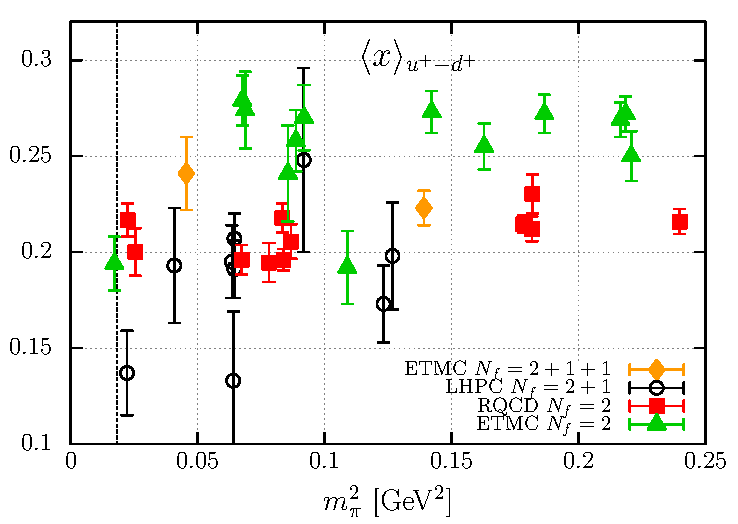
\includegraphics[width=0.49\textwidth]{plots/x_world.pdf}}
\subfloat[]{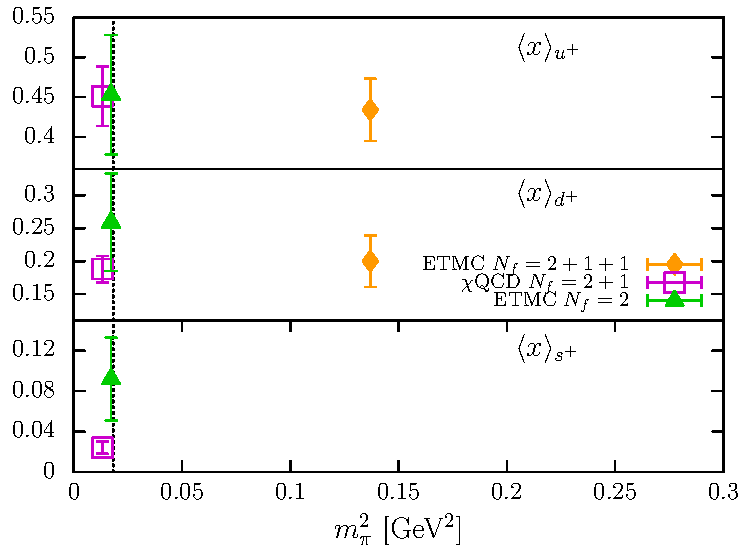
\includegraphics[width=0.47\textwidth]{plots/xq_world_ud.pdf}}
}
\centerline{
\subfloat[]{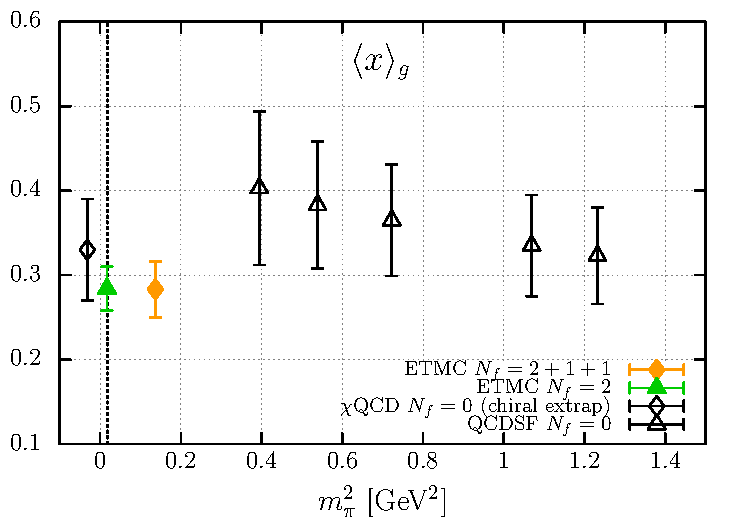
\includegraphics[width=0.49\textwidth]{plots/xg_world.pdf}}
\subfloat[]{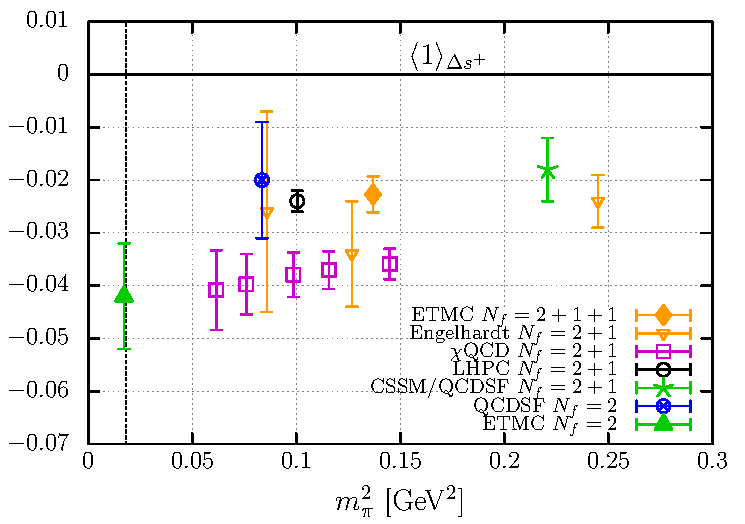
\includegraphics[width=0.49\textwidth]{plots/ga_world_strange.pdf}}
}
\centerline{
\subfloat[]{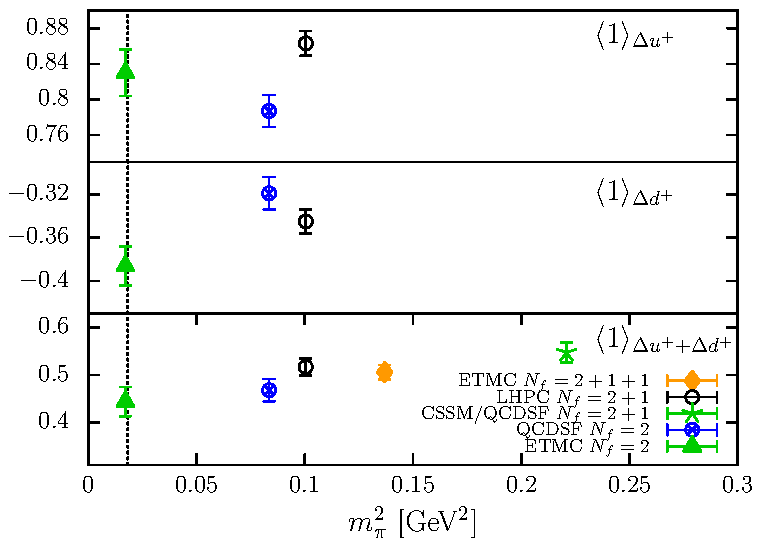
\includegraphics[width=0.49\textwidth]{plots/ga_world_ud.pdf}}
\ \ 
\subfloat[]{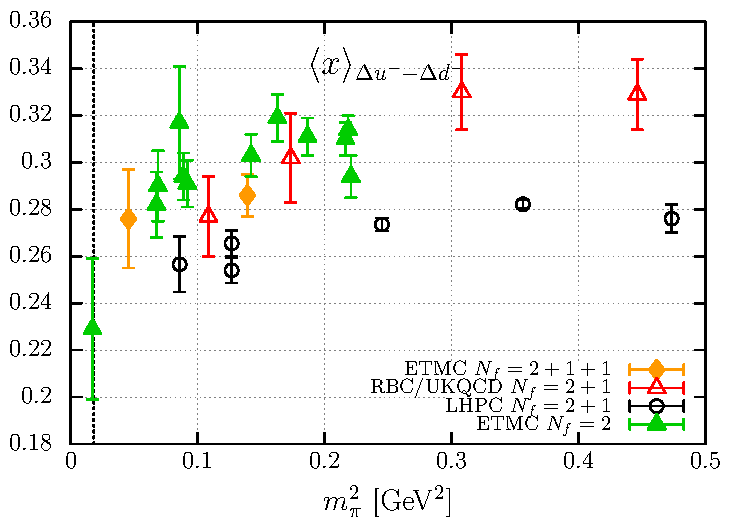
\includegraphics[width=0.49\textwidth]{plots/xdeltaq_isovector.pdf}}
}
\end{center}
\caption{\small Comparison of lattice-QCD results for
  the zeroth and first moments
  of unpolarized and polarized PDFs.
  %
  From left to right and from top to bottom, we show
  results for $\la x\ra_{u^+-d^+}$, $\la x\ra_{q^+}$, $\la x\ra_{g}$,
  $\la 1 \ra_{\Delta s^+}$, $\la 1\ra_{\Delta q^+}$ and
  $\la x\ra_{\Delta u^- - \Delta d^-}$;
  see Tables~\ref{tab:unpolLQCDstatus1}, \ref{tab:polLQCDstatus0},
  \ref{tab:polLQCDstatus1}, \ref{tab:unpolLQCDstatus1B},
  \ref{tab:polLQCDstatus1B} and \ref{tab:polLQCDstatus2B}
  for details.
}
\label{fig:latt_res}
\end{figure}
%-------------------------------------------------------------------------------








% The bibliography
\bibliography{PDFLattice2017}


\end{document}

%%%%%%%%%%%%%%%%%%%%%%%%%%%%%%%%%%%%%%%%%%%%%%%%%%%%%%%%%%%%%%%%%%%%%%%%%%%%%%%%
